% LaTeX support: latex@mdpi.com 
% In case you need support, please attach all files that are necessary for compiling as well as the log file, and specify the details of your LaTeX setup (which operating system and LaTeX version / tools you are using).

% You need to save the "mdpi.cls" and "mdpi.bst" files into the same folder as this template file.

%=================================================================
\documentclass[symmetry,article,accept,moreauthors,pdftex10pt,a4paper]{mdpi} 
%\documentclass[symmetry,article,accept,moreauthors,10pt,a4paper]{mdpi} 

\usepackage{subcaption}
\usepackage{array}
\usepackage{booktabs}
\usepackage{multirow}

\newcommand{\figuresWidth}{0.65\textwidth}

%=================================================================
\firstpage{1} 
\makeatletter 
\setcounter{page}{\@firstpage} 
\makeatother 
\articlenumber{x}
\doinum{10.3390/------}
\pubvolume{xx}
\pubyear{2017}
\copyrightyear{2017}
\history{Received: 31 August 2017; Accepted: 23 November 2017; Published: date }


\usepackage{soul,upgreek}
\usepackage{microtype}


\setitemize{parsep=6pt,itemsep=0pt,leftmargin=*,labelsep=5.5mm}
\setenumerate{parsep=6pt,itemsep=0pt,leftmargin=*,labelsep=5.5mm}
\setlist[description]{itemsep=0mm}


\usepackage[labelformat=simple]{subcaption}
\renewcommand\thesubfigure{\alph{subfigure}}
\DeclareCaptionLabelFormat{subcaptionlabel}{\normalfont(\textbf{#2}\normalfont)}
\captionsetup[subfigure]{labelformat=subcaptionlabel}

%=================================================================
% Full title of the paper (Capitalized)
\Title{Internet of Things: A Scientometric Review\\ 
	{\small \color{blue} NOTE: this is a modifed version to show ScientoPy commands usage}}

% Author Orchid ID: enter ID or remove command
\newcommand{\orcidauthorA}{0000-0001-5896-7618} % Add \orcidONE{} behind the author's name
\newcommand{\orcidauthorB}{0000-0002-1338-8820}
\newcommand{\orcidauthorC}{0000-0001-7993-0240}
\newcommand{\orcidauthorD}{0000-0001-8101-4655}
\newcommand{\orcidauthorE}{0000-0002-8550-0885}


\makeatletter 
  \renewcommand\verbatim@font{\normalfont\ttfamily\color{blue}}
\makeatother



% Authors, for the paper (add full first names)
\Author{Juan Ruiz-Rosero $^{1,}$*\orcidA{}, Gustavo Ramirez-Gonzalez $^{1}$\orcidB{},
	Jennifer M. Williams $^{2}$\orcidC{}, Huaping~Liu~$^{2}$,~Rahul Khanna $^{3}$\orcidD{} and Greeshma Pisharody $^{3}$\orcidE{}}

% Authors, for metadata in PDF
\AuthorNames{Juan Ruiz-Rosero, Gustavo Ramirez-Gonzalez, Jennifer M. Williams, 
Huaping Liu, Rahul Khanna, Greeshma Pisharody}

% Affiliations / Addresses (Add [1] after \address if there is only one affiliation.)
\address{%
$^{1}$ \quad Departamento de Telemática, Universidad del Cauca, Popayán, Cauca 190002, Colombia; gramirez@unicauca.edu.co\\  
$^{2}$ \quad School of Electrical Engineering and Computer Science, Oregon State University, Corvallis, OR 97331, USA; jenmarie@ieee.org (J.M.W.); huaping.liu@oregonstate.edu (H.L.)\\    %%Please add post code after the abbreviation of US State.
$^{3}$ \quad Intel Corporation, 2111 NE 25th Ave., Hillsboro, OR 97124, USA; rahul.khanna@intel.com (R.K.); greeshma.pisharody@intel.com (G.P.) 
}

% Contact information of the corresponding author
\corres{Correspondence: jpabloruiz@unicauca.edu.co; Tel.: +57-(2)-820-9900}

% Simple summary
%\simplesumm{}

% Abstract (Do not use inserted blank lines, i.e. \\) 
%\abstract{A single paragraph of about 200 words maximum. For research articles, abstracts should give a pertinent overview of the work. We strongly encourage authors to use the following style of structured abstracts, but without headings: 1) Background: Place the question addressed in a broad context and highlight the purpose of the study; 2) Methods: Describe briefly the main methods or treatments applied; 3) Results: Summarize the article's main findings; and 4) Conclusion: Indicate the main conclusions or interpretations. The abstract should be an objective representation of the article, it must not contain results which are not presented and substantiated in the main text and should not exaggerate the main conclusions.}

\abstract{Internet of Things (IoT) is connecting billions of devices to the Internet. These IoT devices chain sensing, computation, and communication techniques, which facilitates remote data collection and analysis. wireless sensor networks (WSN) connect sensing devices together on a local network, thereby eliminating wires, which generate a large number of samples, creating a big data challenge. This IoT paradigm has gained traction in recent years, yielding extensive research from an increasing variety of perspectives, including scientific reviews. These reviews cover surveys related to IoT vision, enabling technologies, applications, key features, co-word and cluster analysis, and future directions. Nevertheless, we lack an IoT scientometrics review that uses scientific databases to perform a quantitative analysis. This paper develops a scientometric review about IoT over a data set of 19,035~documents published over a period of 15 years (2002--2016) in two main scientific databases (Clarivate Web of Science and Scopus). A Python script called ScientoPy was developed to perform quantitative analysis of this data set. This provides insight into research trends by investigating a lead author's country affiliation, most published authors, top research applications, communication protocols, software processing, hardware, operating systems, and trending topics. Furthermore,~we~evaluate the top trending IoT topics and the popular hardware and software platforms that are used to research these trends.}

% Keywords: Three to ten pertinent keywords need to be added after the abstract. We recommend that the keywords are specific to the article, yet reasonably common within the subject discipline.
\keyword{Internet of Things; IoT; bibliometric; scientometric; ScientoPy; Web of Science; Scopus; applications; smart environments; communication protocols}



\begin{document}

\section{Introduction}

Internet of Things (IoT) connects billions of devices to the Internet and has gained tremendous popularity in the past decade as a diverse and pioneering technology. In general, IoT devices combine sensing, computation, and communication techniques to deliver remote data collection and system control. Today, these ``things'' range from everyday consumer electronics to specialized industrial systems \cite{8064227}, such as fitness-tracking wristwatches \cite{Hiremath2015304}, transport logistics \cite{Williams2017a}, and smart cars \cite{Gerla2014241} to manufacturing \cite{Bi20141537} and smart grids \cite{Spano2015468}. Contingent on implementation, an IoT device may be used for real-time alerts, data archiving, trend analysis, and forecasting by leveraging related technologies such as cloud services \cite{ibm2015}. Furthermore, the technology has proven useful for small- and large-scale networks, generating a vast portfolio of enabling hardware and software at various complexities \cite{GARCIASANCHEZ2011288,7172291}. IoT technology has led to solutions in use-cases ranging from smart appliances, utilities, biomedical, industrial, data center management, agriculture, body area networks (BANs), surveillance, and more.

Proliferation of IoT research has contributed to increased availability, affordability, responsiveness, diversity, miniaturization, mobility, and more. Recent studies have demonstrated that IoT, cloud~computing, and mobile solutions are among the top technologies that will shape our future in the next 3--5 years \cite{ibm2015}. Not surprisingly, connectivity and intelligence are becoming a contributing factor to many designs fueling advanced development. Therefore, the number of new designs and publications categorized under IoT continues to grow exponentially.

Evolution of IoT has spearheaded many research fields such as wireless sensor networks (WSNs), Big Data, and cloud computing. Wireless Sensor Networks (WSN) comprise: sensor nodes, specialized~firmware \cite{ruiz2014firmware}, relay devices, and data sinks called a gateway. In addition to facilitating data archiving and local processing, the gateway also acts as a hub that connects to the worldwide web for cloud storage and services using a WiFi or cellular network.The computational complexity of analysis and functional use of the data towards trend and forecasting has grown rapidly, such as in the data center management use-cases \cite{6957004}. The radio frequency (RF) communication protocols and the interaction between these sensor entities continue to place stringent hardware requirements. Implementations using one software stack over another could achieve better range, quality-of-service (QoS), and spectral efficiency, at the expense, however, of additional processing, storage, power, and~form-factor \cite{7172291}. Additionally, the connectivity and archiving with WSN results in a large volume of samples that create a ``big data'' challenge. 

\textls[-10]{While IoT is not a new paradigm, it is gaining traction in recent years around the world and yielding extensive research from diverse perspectives. As a result, IoT and similar technologies are progressively challenging topics to review. Starting in 2010, Atzori et al. made a survey about IoT enabling technologies and applications \cite{Atzori20102787}. Then, in 2013, Gubbi et al. defined a cloud center vision for worldwide implementation of IoT, describing the key enabling technologies, applications domains and future directions \cite{Gubbi20131645}. In 2014, Borgia presented an extended review about IoT key features, driving~technologies and protocols, applications, challenges, IoT initiatives, and research directions~\cite{Borgia20141}. Next, in 2015, Yan~et~al. developed a co-word analysis, generating seven clusters that represented the intellectual structure of IoT, which were analyzed by a co-occurrence matrix~\cite{Yan2015}. The~following year, in~2016, Mishra~et~al. composed a bibliometric study about the future vision, applications, and~challenges of Internet of Things~\cite{Mishra20161331}. In~that review, Mishra et al. identified the top contributing authors, key~research topics, most influential works, and emerging research clusters, limited only to future vision and applications of IoT, from a sample of 1556 papers from the Scopus database. }

As noted above, when conducting a review of IoT publications in recent years, the outcome may vary depending on methodology and time spent browsing through search results. At a minimum, only publications of reputable categories from credible databases should be considered for the review process. For example, conference papers, journal articles, proceedings papers, and reviews are widely accepted as reliable information sources in the industry and academia. Additionally, the manual labor of searching thousands of bibliographic data can be reduced by scripting to facilitate the filtering and comparison activities. This allows the reviewer additional time to investigate supplementary metrics in order to render stronger and methodological conclusions.

Therefore, this paper presents a methodology for citation analysis using search results produced by two scholarly bibliographic databases: Clarivate Web of Science (WoS) and Scopus. To facilitate a thorough review of several thousand publications related to IoT, the study presented herein utilized a novel literature review script called ScientoPy to analyze document bibliographies according to predefined metrics. This scientometrics analysis provides insight into research trends in IoT over recent years by investigating a lead author's country affiliation, most published authors, and prevalence of various research topics. Using the authors' keywords, the research topics inspected in this review include applications, communication protocols, software processing, hardware, operating systems, and trending topics. 

%%%%%%%%%%%%%%%%%%%%%%%%%%%%%%%%%%%%%%%%%%
\section{Materials and Methods}

Scientometrics is the study of measuring and analyzing scientific literature by measuring the impact of the innovation and understanding the relevance of these scientific citations to this innovation~\cite{DBLP:journals/corr/abs-1208-4566}. Thus, a Python script for scientometrics literature review (ScientoPy) was developed by the authors to analyze content of publications related to the Internet of Things. This ScientoPy script has the capability to: 

\begin{itemize}
	\item Read Clarivate Web of Science and Scopus databases (.CSV files).
	\item Filter publications by document type.
	\item Find and remove duplicated documents.
	\item Graph the history of the top topics (keywords, authors, countries).
	\item Graph the history of selected items inside a topic.
	\item Find trending topics using the top average growth rate (AGR). 
    \item Calculate the h-index for authors and countries. 
\end{itemize}

ScientoPy is a Python script that automatically generates and reports the top topics (based on authors' keywords), authors, and countries, along with related documents. This automatic data synthesis avoids potential bias as in individual studies. Nevertheless, author name analysis (such as author top list) has a risk of bias across the studies due to possible similarities in names. The writers of this review know and warn about this possibility of documents' author names similarity, which is part of the limitation of any scientometrics study; thus, in this moment not all the authors and data bases have a unique author identifier, like the ORCID, associated with all entries.

\subsection{Data Set}

This scientometrics analysis used two bibliographic databases: Clarivate Web of Science (WoS), and Scopus. For the span of 1 January 2002 to 31 December 2016, the following document types were~studied:

\begin{itemize}
	\item Conference Paper;
	\item Article; 
	\item Review;
	\item Proceedings Paper.
\end{itemize}

The search string for this analysis was ``Internet of Things''. This string was applied to the topic search in WoS and Scopus, which includes title, abstract, authors' keywords, and KeyWords Plus$^{\textregistered}$ (for WoS). With this search criteria, the data set was extracted within a day on 6 July 2017. Table \ref{table_dataset} describes the number and type of documents found in the two databases totaling 27,120 documents. 

\begin{table}[H]
	\centering
	\caption{Type of documents found with the search string ``Internet of Things'' found in  Clarivate Web of Science (WoS) and Scopus within one day on 6 July 2017.}
	\label{table_dataset}
	\begin{tabular}{cccccc}
		\toprule
		\multicolumn{1}{c}{\textbf{Source}} & \textbf{Article} & \textbf{\begin{tabular}[c]{@{}c@{}}Conference \\ Paper\end{tabular}} & \textbf{\begin{tabular}[c]{@{}c@{}}Proceedings \\ Paper\end{tabular}} & \textbf{Review} & \textbf{\begin{tabular}[c]{@{}c@{}}Duplicated \\ Removed\end{tabular}} \\
		\midrule
		WoS    & 3112   &     0    & 8215    & 130   &55    \\
		Scopus & 5283   & 10,068    &    0    & 312   &8030  \\
		\bottomrule
	\end{tabular}
\end{table}

\noindent
\textcolor{brown}{To get the previous table, run the following script, and find the results on ScientoPy/dataPre/PreprocessedBrief}\\
\hspace*{0.5cm}\verb|python preProcess.py dataIn|


\subsection{Pre-Processing}

A pre-processing technique was applied to improve reliability and precision, as detailed in the following sub sections.

\subsubsection{Simplify Author's name}

In general, scientific and bibliographic databases have the following inconsistencies in authors~names:

\begin{itemize}
\item Most journals abbreviate the author's first name to an initial and a dot.
\item Most journals use the author name's special accents.
\item WoS uses a comma between the author's last name and first name initial, but Scopus does not. 
\end{itemize} 

These name-related inconsistencies mean that scientometrics scripts cannot find all of the similar author's names. For that reason, ScientoPy script applies the following steps to simplify author's name fields:

\begin{itemize}
\item Remove dots and coma from author's name.
\item Remove special accents from author's name.
\end{itemize}

\subsubsection{Remove Duplicate Samples}

Of the 27,120 original samples, only 72\% have an associated DOI for uniqueness. Therefore,~duplicated~samples were identified by identical title and authors. For duplicated samples in different databases, the WoS publication was kept and the Scopus sample was removed from the set, resulting in remaining 19,035 documents. Table \ref{table_dataset} shows the number of documents by type and duplicates removed for each database. 


\subsection{Times Cited and H-Index}

Scopus and WoS databases report the Times Cited Count for each document; however, 47\% of the Counts for the same (duplicate) document differ between sources. In such instances, the ScientoPy script selects the highest Times Cited Count, be it from Scopus or WoS, to assign the most favorable value to each document for this metric. Therefore, the h-index for authors and countries is calculated based on these Times Cited Count for the period 2006 to 2016.

\subsection{Document's Country}

In this study, the document's country was extracted from the primary author's corresponding address. Thus, only one country was associated to each document. Furthermore, some authors use different naming to refer to the same country (such as USA and United States). For that reason, some~country names were replaced based on Table \ref{table_countries_rep}.

\begin{table}[H]
	\centering
	\caption{Documents' countries names replacing table.}
	\label{table_countries_rep}
	\begin{tabular}{cc}
		\toprule
		\multicolumn{1}{l}{\textbf{Original}} & \multicolumn{1}{l}{\textbf{Replacement}} \\
		\midrule
		Republic of China & China \\
		USA & United States \\
		England, Scotland, and Wales & United Kingdom \\
		U Arab Emirates & United Arab Emirates \\
		Russia & Russian Federation \\
		Viet Nam & Vietnam \\
		Trinid \& Tobago & Trinidad and Tobago\\
		\bottomrule
	\end{tabular}
\end{table}

In this data set, 95 documents were missing the author's corresponding address to extract the document's country. These samples were discarded for analyses related to country.

\subsection{General IoT Publications Growth}

The yearly growth of IoT related documents were observed as in Figure \ref{fig_database}a, revealing an exponential growth in both databases (WoS and Scopus), without removing the duplicated documents. Figure \ref{fig_database}b shows the similar growth after removing the duplicated documents.  

\begin{figure}[h]
	\centering
	\begin{subfigure}[b]{0.49\textwidth}
		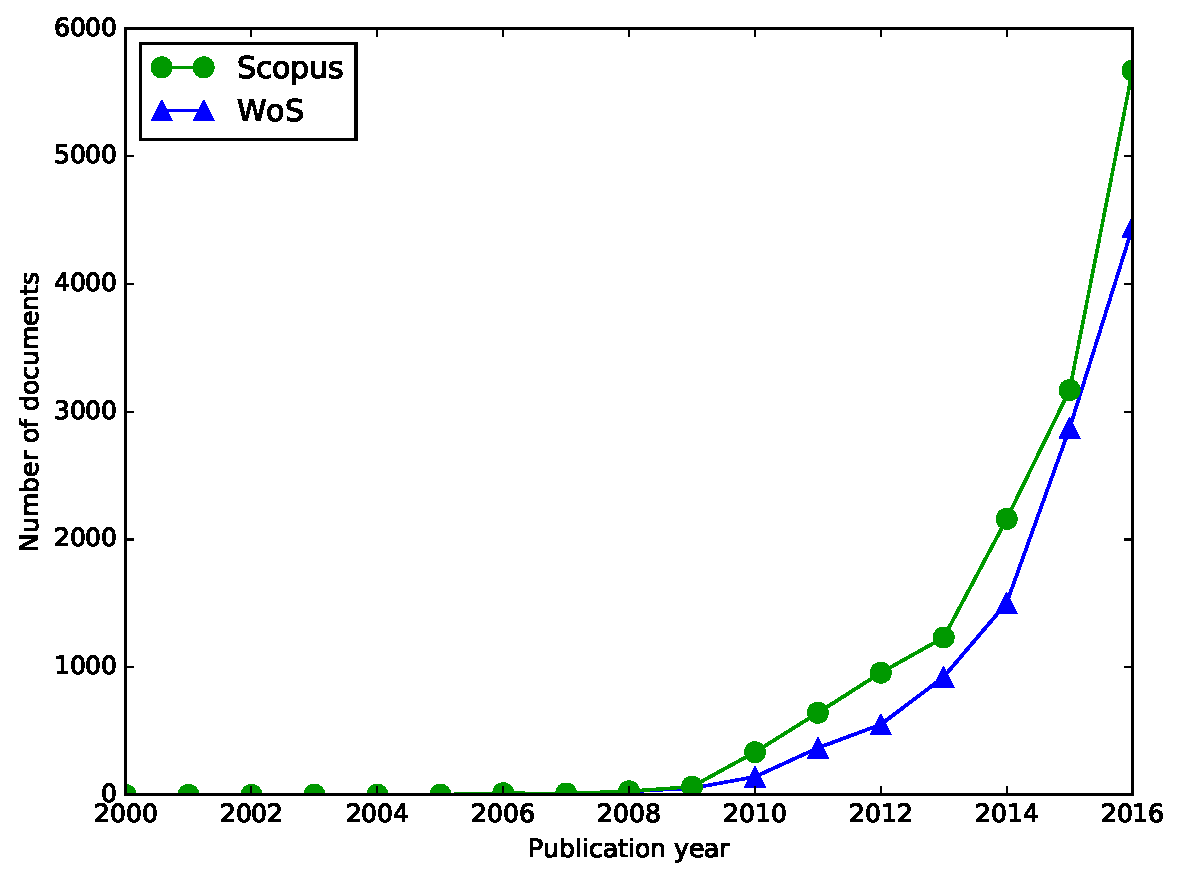
\includegraphics[width=\textwidth]{./graphs/figure1a.eps}
		\caption{}
		\label{fig_database_org}
	\end{subfigure}
	\begin{subfigure}[b]{0.49\textwidth}
		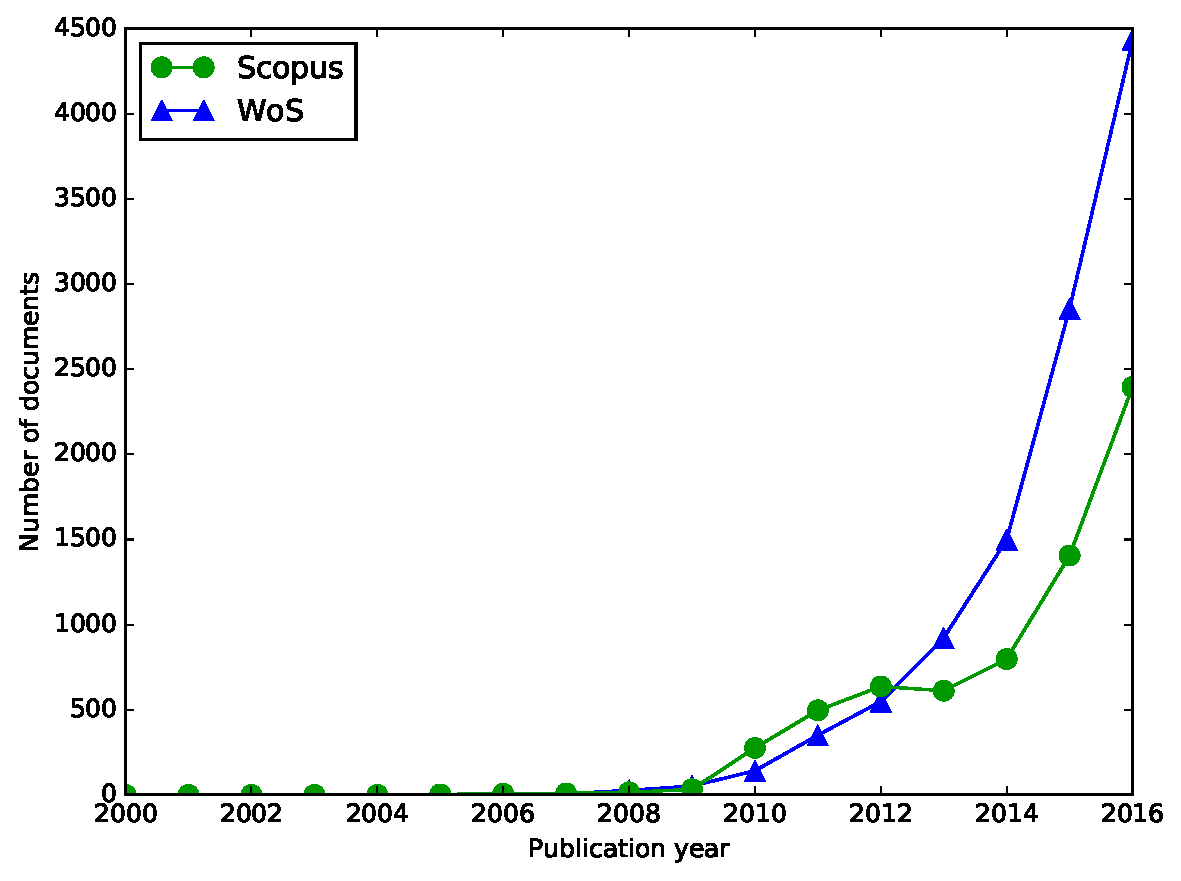
\includegraphics[width=\textwidth]{./graphs/figure1b.eps}
		\caption{}
		\label{fig_database_filtered}
	\end{subfigure}
	\vspace{-12pt}

	\caption{Documents per year published (WoS and Scopus) with the search string ``Internet of Things'' (IoT) for the period 2000 to 2016. (\textbf{a}) before the duplicates-removal filter; (\textbf{b}) after duplicates-removal filter.}\label{fig_database}
\end{figure}

\noindent
\textcolor{brown}{To get the previous figure, run the following script for before the duplicates-removal filter graph:}\\
\hspace*{0.5cm}\verb|python preProcess.py dataIn --noRemDupl|\\
\hspace*{0.5cm}\verb|python scientoPy.py dataBase -t "Scopus;WoS" --savePlot "dataBase_preFilter.eps"|\\

\noindent
\textcolor{brown}{To get the previous figure, run the following script for after duplicates-removal filter graph:}\\
\hspace*{0.5cm}\verb|python preProcess.py dataIn|\\
\hspace*{0.5cm}\verb|python scientoPy.py dataBase -t "Scopus;WoS" --savePlot "dataBase_postFilter.eps"|\\


The first mention of the ``Internet of Things'' was an article published in March 2002 reported by WoS. Published by Forbes, Schoenberger, and Upbin, this article described how the IoT could be a standardized way to help the computers understand the world \cite{ISI:000174207300032}. In 2003, Scopus reported a paper from the Institute of Electrical and Electronics Engineers (IEEE) International Conference on Systems, Man and Cybernetic, in which Qui and Zhang showed the design of enterprise web servers supporting instant data retrieval for a product labeled with an Radio-frequency identification (RFID) based smart tag \cite{Qiu20032661}. Scopus reported a second conference paper in 2003 for the 36th Annual Hawaii International Conference on System Sciences, Traversat et al. on the stated the JXTA (abbreviation of Juxtapose) protocols as a foundation of the upcoming Web of Things\cite{Traversat2003}. 

\textls[-15]{In 2004, WoS and Scopus reported the same two articles: ``The Internet of Things'' by Gershenfeld~et~al.~\cite{Gershenfeld200476}, and ``The Supply Chain'' by Luckett \cite{ISI:000224027400006}. From 2005 to 2016, Scopus reported about 30\% more publications than WoS. Nevertheless, for this research, WoS documents were given more priority over Scopus documents during the duplicates-removal process because WoS fields were more complete than Scopus, such as cited references with Digital Object Identifier (DOI) number and subject category. For this reason, Figure \ref{fig_database}b shows more documents from WoS than Scopus from 2013 onwards.}

\section{Country and Author Research Analysis}

In this section, analysis was focused on authors and their corresponding country. Below is a graph of the percentage of publications related to IoT each year for the seven countries with the highest occurrence in the data set. A table of the most occurring 50 countries is also provided. Another graph presents the top five authors per year, alongside tables detailing the top 20 authors and 10 most cited author documents for articles, conferences and reviews. 

\subsection{Country Analysis}

A list of the countries with the most associated publications was generated. Figure \ref{fig_countries} shows the top seven countries, along with the percentage of documents published per year. In 2002, one article was published on Forbes by Schoenberger; unfortunately, the database does not associate any author address for this document and the sample had to be removed from this data set according to methodology. In 2003, two conference papers were published by United States authors \cite{Qiu20032661,Traversat2003}. In 2004, there was one review publication in the United States \cite{Gershenfeld200476} and one article in the United Kingdom \cite{ISI:000224027400006}. 

\begin{figure}[H]
	\centering
	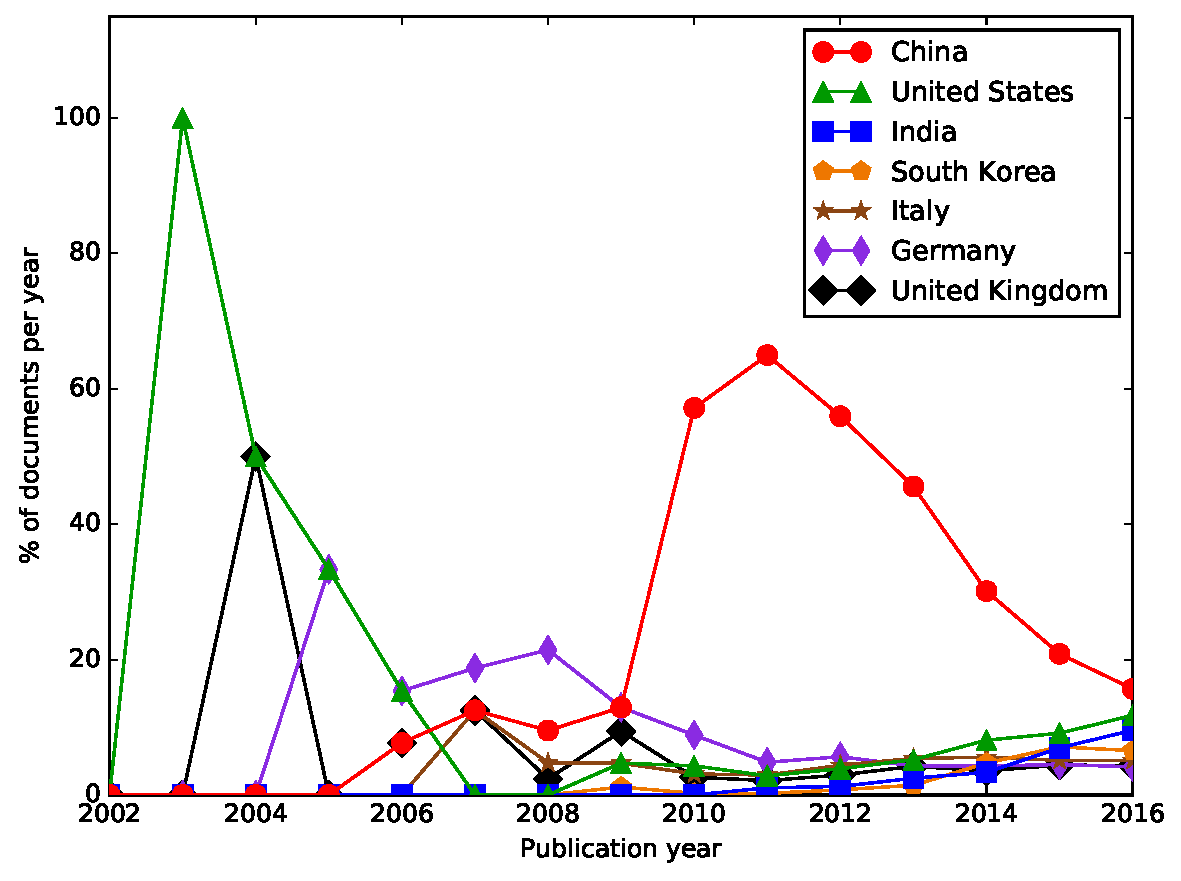
\includegraphics[width=\figuresWidth]{./graphs/figure2.eps}
	\caption{Internet of Things percentage of documents published per year by the top 7 first author's corresponding address country for the period 2002 to 2016.}
	\label{fig_countries}
\end{figure}

\noindent
\textcolor{brown}{To get the previous figure, run the following script:}\\
\hspace*{0.5cm}\verb|python scientoPy.py country --startYear 2002 -l 7 --pYear --savePlot "countries.eps"|\\

Germany \cite{Bose2005} and Malaysia \cite{Norman2005} first appear in 2005, joined by the United States  \cite{Djassemi2005}. These three conference papers demonstrated how the RFID can boost Internet of Things for manufacturing, packing, tracking, and automobile logistics. In 2006, the total publications grew from 3 to 12, with~more countries participating, such as France \cite{4022056,1698342}, Switzerland \cite{Adelmann2006366,Lehtonen200677}, and Japan \cite{Futatsumori2006258}. From 2006 to 2009, Germany led the number of publications with 2, 3, 9, and 11, respectively. During that period, the~German author Broll led the citations count with a proposed framework for integrating web services and mobile interaction with physical objects \cite{5262929}.

China drastically increased from 11 to 239 publications from 2009 to 2010, continuing to contribute more than half of the globally published documents between 2010 to 2013. Most of that growth resulted from China's Twelfth 5 Year Plan (2011--2015), which included the development of the Internet of Things \cite{ISI:000304905300012}. The conference paper ``IOT Gateway: Bridging Wireless Sensor Networks into Internet of Things'' by Zhu was the most
cited IoT paper during this period for China, as it explained how an IoT Gateway could make a bridge between wireless sensors networks and traditional communications networks to the Internet \cite{Zhu2010347}.

From 2014 to 2016, China maintained the highest rank, contributing 20\% of the globally published documents, as well as a peak in 2016 and h-index of 47. In 2014, the United States was second to China with 187 publications and h-index of 42. India's contributions grew at a rate of 153\%, 103\%, 286\%, and 120\%, in 2013 to 2016, respectively, moving from the 8th to 3rd position in 2013 and 2016, respectively. The~Indian daily ``The Economic Times'' forecasted the country is expected to see a rapid 31-fold growth of IoT devices to reach 1.9 billion by 2020 \cite{theEconomicTimes2017}. 


Expanding the results from Figure \ref{fig_countries}, Table \ref{table_countries} shows the top 50 countries of the primary author with the average percentage growth and the h-index of each country from the last three years (2014 to 2016). Of the top 10 countries, South Korea represents the maximum average growth with 206\%, where~the mobile carrier SK Telecom (Seoul, South Korea) launched the first commercial low-cost Internet of Things (IoT) network in 2016 \cite{bbcKorea2016}. However, this growth is not reflected yet (next year) in the available literature and thus the data set has an h-index of 16, only half of its successor in this list, Italy. In the same way, this list includes the top growing countries with low h-index but anticipated to be higher next year: Indonesia, Turkey, Russian Federation, and Pakistan.


\begin{table}[H]
	\centering
	\caption{Internet of Things top 50 countries of first author's corresponding address. Country number position (N.), total number of publications (Total), average percentage growth from the last 3 years (2014 to 2016), and h-index (h-ind.) from 2006 to 2016.}
	\label{table_countries}
	\begin{tabular}{ccccc}
  %  	\cmidrule[0.75pt]{1-5} 		\cmidrule[0.75pt]{7-11}
  \toprule
	{\textbf{N.}} & {\textbf{Country}} &{\textbf{Total}} &{\textbf{Average Growth}} & {\textbf{h-Ind.}} \\
	\midrule
		%\cmidrule[0.4pt]{1-5} 		\cmidrule[0.4pt]{7-11}
		1 & China & 4822 & 16\% & 47 \\
		2 & United States & 1561 & 116\% & 42  \\
		3 & India & 1089 & 169\% & 15  \\
		4 & South Korea & 894 & 206\% & 16   \\
		5 & Italy & 874 & 61\% & 32   \\
		6 & Germany & 811 & 64\% & 24   \\
		7 & United King. & 711 & 71\% & 25  \\
		8 & France & 543 & 126\% & 21  \\
		9 & Spain & 463 & 42\% & 23  \\
		10 & Japan & 449 & 166\% & 11   \\
		11 & Taiwan & 438 & 68\% & 16 \\
		12 & Brazil & 272 & 90\% & 9 \\ 
		13 & Finland & 266 & 50\% & 20 \\ 
		14 & Canada & 259 & 104\% & 15 \\ 
		15 & Australia & 249 & 59\% & 22 \\ 
		16 & Sweden & 216 & 68\% & 17 \\ 
		17 & Switzerland & 193 & 31\% & 19 \\
		18 & Portugal & 191 & 45\% & 13 \\ 
		19 & Greece & 180 & 46\% & 14 \\ 
		20 & Romania & 169 & 72\% & 9 \\ 
		21 & Belgium & 164 & 87\% & 11 \\ 
		22 & Austria & 146 & 113\% & 12 \\ 
		23 & Malaysia & 137 & 71\% & 9 \\ 
		24 & Russian Fed. & 134 & 271\% & 8 \\
		25 & Ireland & 126 & 116\% & 9 \\
		26 & Netherlands & 109 & 122\% & 12 \\
		27 & Singapore & 109 & 112\% & 8\\
		28 & Poland & 104 & 77\% & 6\\
		29 & Czech Rep. & 101 & 153\% & 5\\
		30 & Turkey & 92 & 319\% & 5\\
		31 & Pakistan & 82 & 210\% & 7\\
		32 & Saudi Arabia & 80 & 122\% & 7 \\
		 33 & Norway & 72 & 119\% & 11\\
		34 & UAE & 71 & 180\% & 6\\
		35 & South Africa & 60 & 162\% & 9  \\
		 36 & Denmark & 59 & 39\% & 11 \\
		37 & Tunisia & 55 & 163\% & 6 \\
		38 & Serbia & 53 & $-$1\% & 6 \\
		39 & Croatia & 51 & 159\% & 6 \\
		40 & Hungary & 51 & 24\% & 6 \\
		41 & Indonesia & 51 & 410\% & 3 \\
		42 & Egypt & 49 & 159\% & 4 \\
		43 & Morocco & 47 & 163\% & 4 \\
		44 & Iran & 42 & 94\% & 5 \\
		45 & Colombia & 39 & 146\% & 3 \\
		46 & Algeria & 38 & 113\% & 5 \\
		47 & Jordan & 38 & 108\% & 5 \\
		48 & New Zealand & 38 & 86\% & 6 \\
		49 & Mexico & 36 & 172\% & 5 \\
		50 & Thailand & 32 & 107\% & 4 \\
		\bottomrule
		%\cmidrule[0.4pt]{1-5} 		\cmidrule[0.4pt]{7-11}
	\end{tabular}
\end{table}

\noindent
\textcolor{brown}{To get the previous table, run the following script, and find the results in results/Country.csv:}\\
\hspace*{0.5cm}\verb|python scientoPy.py country --startYear 2002 -l 50 --noPlot|\\


The  International Data Corporation (IDC) predicts that, by 2019, 20\% of local and regional governments in Indonesia will use the Internet of Things to turn infrastructure such as roads, street lights, and~traffic signals into assets instead of liabilities \cite{Estopace2017}. In addition, the Dutch IoT start-up, Xeelas (Arnhem, Netherlands), and~Turkish group, Sade (Ankara, Turkey), partnered to build Turkey's largest LoRaWAN (LoRa, Long Range Wide-area network network) in Istanbul to enable business, local governments, and conservation groups to collect and analyze from connected devices \cite{turkey2017}. In Russia, the Internet of Things market is expected to reach USD 74 Billion by 2023, where the Russian government's Internet start-up fund (FRII) has joined forces with tech giants GS Group (Saint-Petersburg, Russia) and mobile operators to launch a national Internet of Things (IoT) consortium \cite{russia2017}. In Pakistan, by~January~2017, 17~Internet of Things start-ups were launched, on their own or incubated, at Plan9 (Lahore, Pakistan), NEST i/o (Karachi, Pakistan), and~i2i~(Islamabad, Pakistan) \cite{ignite2017}.

 


\subsection{Author Analysis}

The data set analyzed here includes 31,422 authors of the 19,035 documents related to Internet of Things. In addition, 592 of these authors have 10 or more publications in WoS or Scopus. Figure \ref{fig_authors} shows the top five~authors with the most published documents per year. Y. Zhang was positioned first with 130~published documents related to IoT and
RFID, security, electric vehicle, artificial immune system, smart grid, and cloud computing. In 31 documents, Y. Zhang appeared as a first author. His most cited document is the article titled ``Toward Cloud-Based Vehicular Networks with Efficient Resource Management'' \cite{ISI:000325658900009} with 96 citations.

\begin{figure}[H]
	\centering
	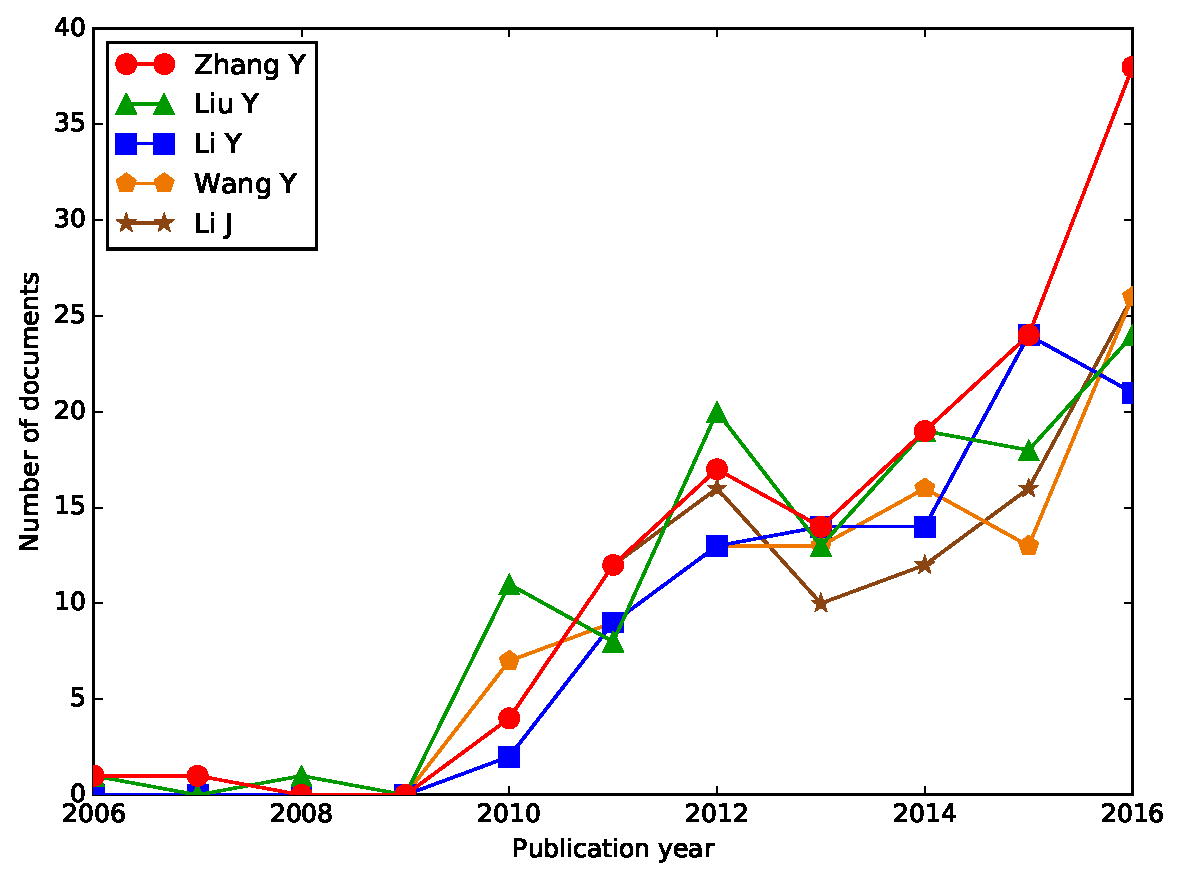
\includegraphics[width=\figuresWidth]{./graphs/figure3.eps}
	\caption{Internet of Things top 5 authors with most documents published per year, for the period 2006 to 2016.}
	\label{fig_authors}
\end{figure}  

\noindent
\textcolor{brown}{To get the previous figure, run the following script:}\\
\hspace*{0.5cm}\verb|python scientoPy.py authors --startYear 2006 -l 5 --savePlot "authors.eps"|\\


Y. Liu is positioned second with 115 documents, of which 36 list him as the primary author. His~publications are more focused on hardware such as Raspberry Pi, test bed, optical communications, ZigBee, and RFID. The article titled ``IOT gateway: Bridging wireless sensor networks into Internet of Things'' is his most cited document with 134 citations \cite{Zhu2010347}. Y. Liu shares the authorship in four~publications with the first author in this list, Y. Zhang.

Y. Li is the third in this list with 97 publications, with 37 as the primary author. His  focus was on RFID, big data, and databases. ``Towards a theoretical framework of strategic decision, supporting capability and information sharing under the context of Internet of Things'' \cite{Li2012} is his most cited publication with 39 citations. With the same number of publications, 97 and 39 as the primary author, Y.~Wang is next in this list. His research is related to RFID, smart gird, security, logistics, and big data. His most cited document is \cite{6737280} with 16 citations. Lastly, fifth on this list is J. Li with 96~publications with 33 as the primary author. His papers related to RFID, ZigBee, and standardized breeding, with his proceedings paper in \cite{Su20111028} being his most cited paper with 97 citations in this set.  %please note this author did not appear in ref 71.

Table \ref{table_top_20_authors} shows the top 20 authors with the most published number of documents, along with the author's h-index in IoT, most cited document, and top research topics. Nevertheless, the two-top h-index authors in this case are not in the top 20 number of documents. L.D. Xu is the author with the highest h-index of 21 and 33 publications. Similarly, L. Atzori has second place in h-index of 14~and 41 documents. 

\begin{table}[H]
	\centering
	\caption{Internet of Things, top 20 authors with most publications, total number of documents, h-index, most cited document, and top related research topics for the period 2006 to 2016.}
	\label{table_top_20_authors}
	\scalebox{.95}[1.0]{\begin{tabular}{cccccc}
		\toprule
		\multicolumn{1}{c}{\textbf{N.}} & \multicolumn{1}{c}{\textbf{Author}} & \multicolumn{1}{c}{\textbf{Total Documents}} & \multicolumn{1}{c}{\textbf{h-Index}} & \multicolumn{1}{c}{\textbf{\begin{tabular}[c]{@{}c@{}}Most Cited \\ Document\end{tabular}}} & \multicolumn{1}{c}{\textbf{Top Author Topics}} \\
		\midrule
		1 & Zhang, Y. & 130 & 12 & \cite{ISI:000325658900009} & RFID, security, Electric vehicle \\
		2 & Liu, Y. & 115 & 11 & \cite{Zhu2010347} & RFID, name service, ZigBee \\
		3 & Li, Y. & 97 & 9 & \cite{Li2012} & RFID, big data, database \\
		4 & Wang, Y. & 97 & 5 & \cite{6737280} & RFID, smart grid, secirity \\
		5 & Li, J. & 96 & 9 & \cite{Su20111028} & RFID, ZigBee, standarized breeding \\ %please note this author did not appear in ref 71.
		6 & Zhang, J. & 82 & 6 & \cite{6649727} & RFID, WSN, monitoring system \\
		7 & Wang, J. & 80 & 8 & \cite{Wang201351} & RFID, 5G, sampling \\
		8 & Zhang, L. & 79 & 13 & \cite{Li2010} & Cloud computing, cloud manufacturing, ZigBee \\
		9 & Wang, X. & 78 & 6 & \cite{Li20131696} & RFID, ZigBee, service selection \\
		10 & Chen, Y. & 72 & 8 & \cite{Chen201481} & RFID, WSN, ZigBee \\
		11 & Jara, A.J. & 72 & 13 & \cite{ISI:000288757900012} & 6LoWPAN, smart cities, big data \\
		12 & Zhang, X. & 72 & 6 & \cite{Yang2015161} & Logistics, RFID, WSN \\
		13 & Li, H. & 71 & 7 & \cite{Li2015} & RFID, authentication, security \\
		14 & Wang, H. & 70 & 9 & \cite{Qin2016137} & RFID, monitoring, cloud computing \\
		15 & Li, X. & 67 & 8 & \cite{Li201168} & RFID, recommendation, smart grid \\
		16 & Liu, J. & 65 & 10 & \cite{Sun20101} & Cloud computing, RFID, security \\
		17 & Kim, J. & 62 & 7 & \cite{Lim2015375} & WSN, video streaming, HEVC \\
		18 & Wang, Z. & 60 & 8 & \cite{Guo20131531} & RFID, GPRS, EPC network \\
		19 & Liu, X. & 59 & 9 & \cite{Li20131147} & Cloud computing, RFID, Landsenses ecology \\
		20 & Kim, D. & 58 & 7 & \cite{Hong201034} & EPCIS, 6LoWPAN, security \\
    	\bottomrule
	\end{tabular}}
\end{table}

\noindent
\textcolor{brown}{To get the previous table, run the following script, find the results in results/Authors\_extended.csv and results/Authors.csv, read the keywords and some papers to extract manually the top author topics}\\
\hspace*{0.5cm}\verb|python scientoPy.py authors --startYear 2006 -l 20 --noPlot|\\


Table \ref{table_times_cited} shows the most cited papers for three document types (articles, conference/proceedings and reviews). Atzori et al. surveys IoT vision and enabling technologies \cite{Atzori20102787}. Second in articles, Gubbi~et~al. describe a cloud-centered vision for the worldwide implementation of IoT \cite{Gubbi20131645}. Miorandi~et~al.'s article surveys on technologies, applications and research challenges for IoT \cite{Miorandi20121497}. 
For conferences and proceedings, Bonomi et al. describe the Fog computing characteristics and its role in IoT \cite{Bonomi201213}. Tao et al. propose cloud computing, Internet of Things, virtualization, and service-oriented combination technologies with advanced manufacturing models and enterprise information technologies to generate a new manufacturing model, called cloud manufacturing (CMfg)~\cite{Tao20111969}. Tan and Wang show a skeleton of the Internet of Things with an application model that can apply to automatic facilities management in the smart campus \cite{Tan2010}.

Finally, on the reviews side, Gershenfeld et al. present a review about the Internet-0 (Internet-Zero) protocol, whose approach for the reduced complexity of the IP stack extends the notion of internetworking to interdevice \cite{Gershenfeld200476}. Meng and Ci mention that the data type and amount is growing at a high speed due to emerging  services such as cloud computing, IoT, and social media. Thus,~they~review the concept of big data and describe a new era for data handling \cite{Meng2013146}. Lastly, Aziz et al. surveys the topology control techniques for extending the lifetime of battery to power WSNs for the Internet of Things battery-powered devices \cite{Aziz2013121}.

\begin{table}[H]
	\centering
	\caption{Internet of Things top 10 documents with most citations, divided by document type, including~position number (N.), first author, document reference, times cited, publication year, and~first author corresponding address for the period 2002 to 2016.}
	\label{table_times_cited}
	\begin{tabular}{cccccc}
	\toprule
	\textbf{N.} & \multicolumn{1}{c}{\textbf{First Author}} & \multicolumn{1}{c}{\textbf{\begin{tabular}[c]{@{}c@{}}Document\\ Reference\end{tabular}}} & \multicolumn{1}{c}{\textbf{\begin{tabular}[c]{@{}c@{}}Times \\ Cited\end{tabular}}} & \textbf{\begin{tabular}[c]{@{}c@{}}Publication \\ Year\end{tabular}} & \textbf{Country} \\
    \midrule
	\multicolumn{6}{l}{Articles documents} \\
    \midrule
	1 & Atzori L & \cite{Atzori20102787} & 3239 & 2010 & Italy \\
	2 & Gubbi J & \cite{Gubbi20131645} & 1369 & 2013 & Australia \\
	3 & Miorandi D & \cite{Miorandi20121497} & 721 & 2012 & Italy \\
	4 & Kortuem G & \cite{Kortuem201044} & 506 & 2010 & United Kingdom \\
	5 & Ganti RK & \cite{Ganti201132} & 494 & 2011 & United States \\
	6 & Bobadilla J & \cite{Bobadilla2013109} & 482 & 2013 & Spain \\
	7 & Li B-H & \cite{Li2010} & 471 & 2010 & China \\
	8 & Perera C & \cite{Perera2014414} & 454 & 2014 & Australia \\
	9 & Zanella A & \cite{Zanella201422} & 404 & 2014 & Italy \\
	10 & Chen M & \cite{Chen2014171} & 370 & 2014 & China \\  \midrule
	\multicolumn{6}{l}{Conference and proceedings documents} \\
    \midrule
	1 & Bonomi F & \cite{Bonomi201213} & 508 & 2012 & United States \\
	2 & Tao F & \cite{Tao20111969} & 228 & 2011 & China \\
	3 & Tan L & \cite{Tan2010} & 169 & 2010 & China \\
	4 & Spiess P & \cite{Spiess2009968} & 156 & 2009 & Not specified \\
	5 & Mainetti L & \cite{Mainetti201116} & 142 & 2011 & Italy \\
	6 & Zhu Q & \cite{Zhu2010347} & 134 & 2010 & China \\
	7 & Dohr A & \cite{Dohr2010804} & 132 & 2010 & Austria \\
	8 & Kovatsch M & \cite{Kovatsch2011855} & 112 & 2011 & Switzerland \\
	9 & Khan R & \cite{Khan2012257} & 101 & 2012 & Italy \\
	10 & Su KH & \cite{Su20111028} & 97 & 2011 & China \\  \midrule
	\multicolumn{6}{l}{Review documents} \\
    \midrule
	1 & Gershenfeld N & \cite{Gershenfeld200476} & 271 & 2004 & United States \\
	2 & Meng X & \cite{Meng2013146} & 172 & 2013 & China \\
	3 & Aziz AA & \cite{Aziz2013121} & 139 & 2013 & Malaysia \\
	4 & Domingo MC & \cite{Domingo2012584} & 138 & 2012 & Spain \\
	5 & Borgia E & \cite{Borgia20141} & 132 & 2014 & Italy \\
	6 & Hancke GP & \cite{Hancke2013393} & 101 & 2013 & South Africa \\
	7 & Wang ZL & \cite{Wang2010320} & 98 & 2010 & United States \\
	8 & Wang SH & \cite{Wang2015436} & 83 & 2015 & United States \\
	9 & Keoh SL & \cite{Keoh2014265} & 69 & 2014 & Singapore \\
	10 & Malhotra A & \cite{Malhotra20131265} & 64 & 2013 & United States\\
   	\bottomrule
	\end{tabular}
	\end{table}

\noindent
\textcolor{brown}{To get the previous table, open on a spreadsheet editor the results/papersPreprocessed.csv file, short the documents by document type, and then by cited by.}


\section{Research Topics}

IoT has a broad spectrum of research fields such as applications, smart objects, communications protocols, software processing, devices hardware, and operating systems. On the data set analyzed here, most of the authors include their research topic in the document keywords. In this section, author~keywords were analyzed to find the trends in the different research topics. For Scopus, the regular authors' keywords were used, and similarly for WoS. KeyWords Plus from WoS were discharged because they are index terms created automatically from significant, frequently occurring words in the titles of an article's cited references, and they are less comprehensive in representing an article's content \cite{zhang2016comparing}. The top 1000 keywords were extracted, manually classified in the different research field, and grouped by plural-singular similarity and/or abbreviations. For instance, the keywords WSN, wireless sensor network, and wireless sensor networks were grouped into the WSN keyword. The following subsections describe the trend of the research topics in different fields, based on the top authors' keywords publications per year. Figure \ref{fig_keywords} shows the general top 10 authors' keywords.

\begin{figure}[H]
	\centering
	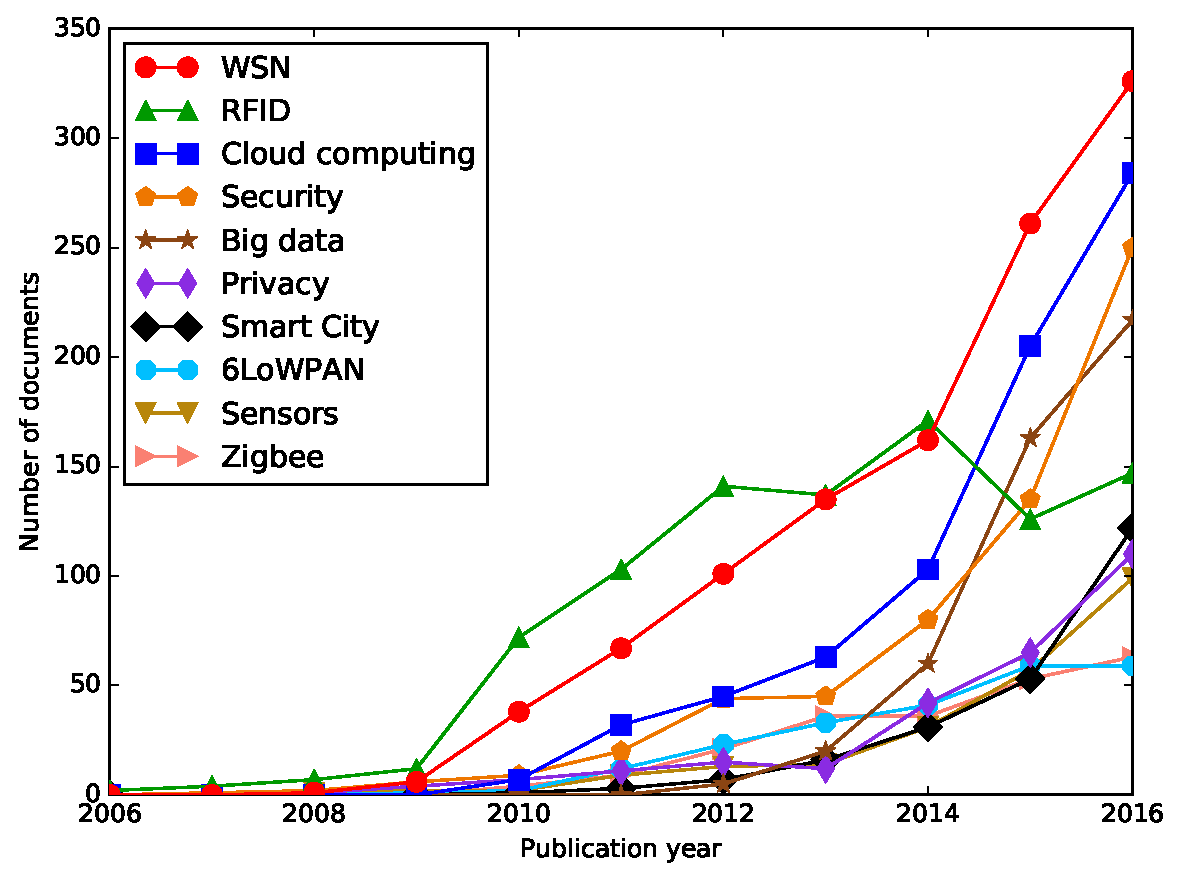
\includegraphics[width=\figuresWidth]{./graphs/figure4.eps}
	\caption{Internet of Things top authors' keywords documents published per year, excluding the keywords: Internet of Things, IoT, Internet of Things (IoT), and The Internet of Things, for the period 2006 to 2016.}
	\label{fig_keywords}
\end{figure} 

\noindent
\textcolor{brown}{To get the previous figure, run the following script:}\\
\begin{verbatim}
python scientoPy.py authorKeywords -t \
"WSN,Wireless sensor network,Wireless sensor networks; \
RFID,RADIO FREQUENCY IDENTIFICATION;Cloud computing;Security;Big data; \
Privacy;Smart City;6LoWPAN;Sensors;Zigbee" --startYear 2006 --savePlot "keywords.eps"
\end{verbatim}

  
\subsection{Applications}

There are several application fields related to IoT research and development. In this section, the~authors' keywords were analyzed to find the top specified applications. Figure \ref{fig_applications} shows the trend of these applications in documents per year. Furthermore, Figure \ref{fig_applications}a presents the applications that start with the word ``smart'', and Figure \ref{fig_applications}b those that do not.

\begin{figure}[H]
	\centering
	\begin{subfigure}[b]{0.49\textwidth}
		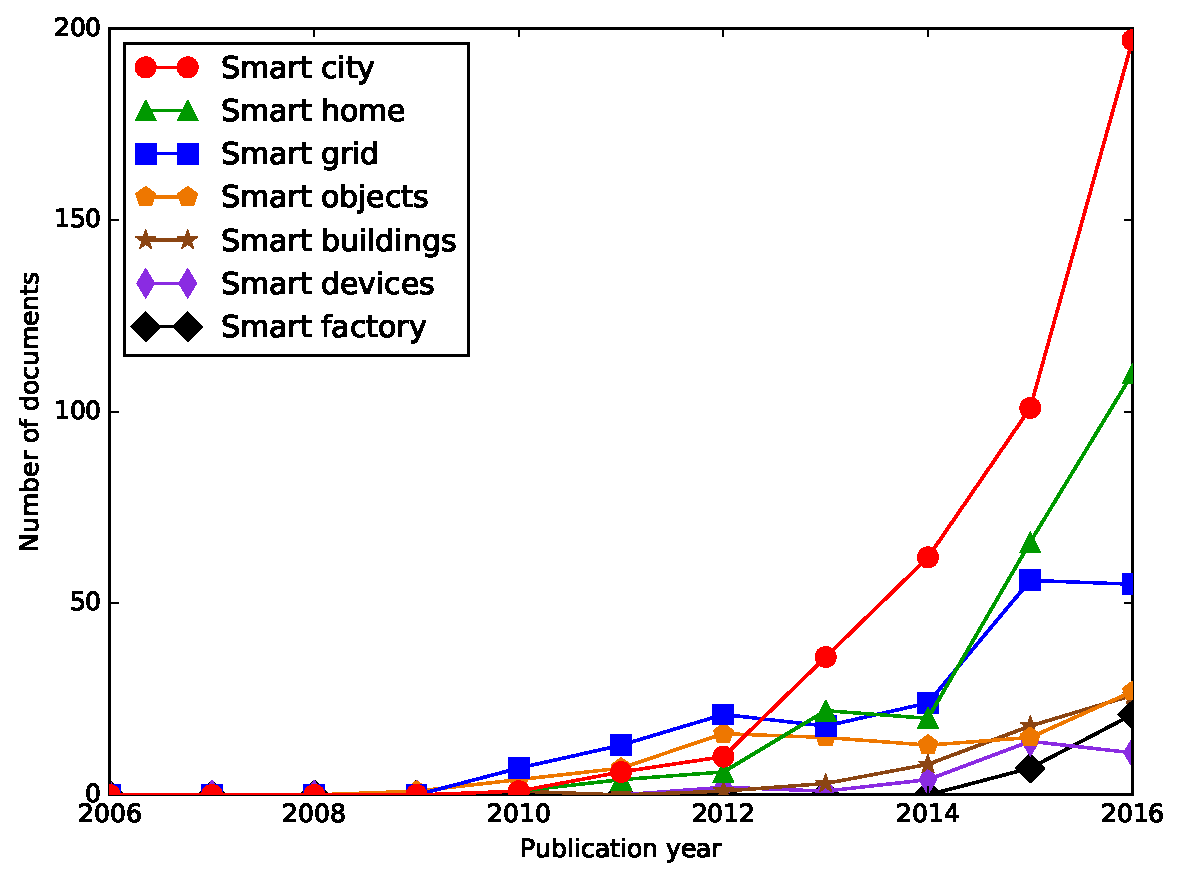
\includegraphics[width=\textwidth]{./graphs/figure5a.eps}
		\caption{}
		\label{fig_smart_things}
	\end{subfigure}
	\begin{subfigure}[b]{0.49\textwidth}
		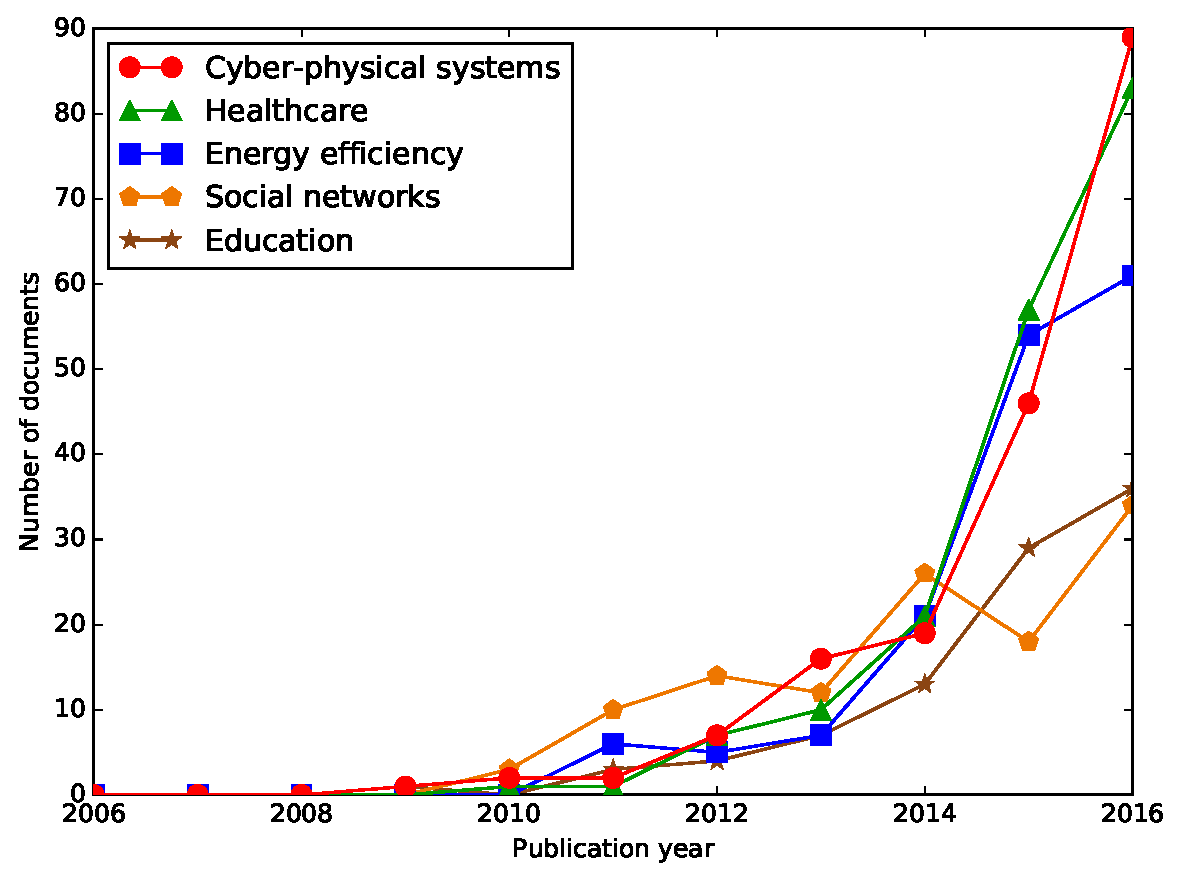
\includegraphics[width=\textwidth]{./graphs/figure5b.eps}
		\caption{}
		\label{fig_applications_a}
	\end{subfigure}
	\vspace{-12pt}

	\caption{Internet of Things top applications based authors' keywords in documents per year, for the period 2006 to 2016.  (\textbf{a}) applications that start with ``smart'' (\textbf{b}) applications that do not start with~``smart''.}
	\label{fig_applications}
\end{figure}

\noindent
\textcolor{brown}{To get the previous figure, run the following script for smart applications:}\\
\begin{verbatim}
python scientoPy.py authorKeywords -t \
"Smart city,Smart cities;Smart home,Smart homes;Smart grid,Smart grids;\
Smart objects,Smart object,Smart enviroments,Smart enviroment;\
Smart buildings,Smart Building;Smart devices;Smart factory" \
--startYear 2006 --savePlot "smart_things.eps"
\end{verbatim}

\noindent
\textcolor{brown}{To get the previous figure, run the following script for not start smart applications:}\\
\begin{verbatim}
python scientoPy.py authorKeywords -t \
"Cyber-physical systems,CYBER PHYSICAL SYSTEMS,CPS;\
Healthcare,E-Health;Energy efficiency;\
Social networks,Social networks,Social media;\
Education,Learning,E-Learning,mobile learning" \
--startYear 2006 --savePlot "applications.eps"
\end{verbatim}

In the data set, 1052 documents were found for applications that start with ``smart''. Smart~city is the top one in this list, with 413 documents, and a sigmoid growth in exponential phase, 95\%~more publications in 2016 vs. 2015. A.J. Jara has the most number of documents in this field with 12~publications. His most cited document \cite{7406686} refers to Smart and Connected Communities as a concept that is evolving from Smart cities. The leading country in this application is Italy with 50~publications, and the most important correlated topics are Big data \cite{Li2014631,Moreno-Cano2015418,GomezRomero2016}, Cloud computing~\cite{Kaur2016,Chang201642}, and Smart grid~\cite{Longo2014458,Longo2015281}. Similarly, Smart home has a linear growth, with 230 documents, and~111 in the last year, with China as the leading country. The most important related topics for Smart home are security~\cite{UlRehman2016,Alohali2014115,Peter2017}, ZigBee \cite{Peng2016335,Yiqi2014114,Gong201689}, and activity recognition \cite{Cicirelli2016,Bourobou201511953,Fortino2015}.

In contrast, smart grid is a topic that has not demonstrated continuous growth. In 2012--2013, the documents published per year decreased from 21 to 13, and in 2015--2016 from 56 to 55. Nevertheless,~an~overall 194 documents were registered on this topic, with China as the leading country. The~term smart grid refers to ``a next generation power grid that uses two-way flows of electricity and information to create a widely distributed automated energy delivery network'' \cite{Fang2012944}. Within IoT, the research on smart grids are related to  security \cite{Noll2014371,Pitas2014231,Dalipi201663}, cloud computing \cite{Meloni2016387,Wang20111}, and privacy \cite{Beligianni2016,Winter201545,Dalipi201663}.

\textls[-15]{According to Dumitrache, ``Cyber-Physical Systems (CPS)s are physical, biological and engineered systems whose operations are monitored, coordinated, controlled and integrated by a computing and communication core'' \cite{Dumitrache20103}. Publications of this topic related to IoT have a sigmoid growth in exponential phase, with 182 publications in 2016, noting United States as the leading country with 34~documents. The~most important related topics are: Industry 4.0 \cite{Jazdi2014,7733506,Zhou2016167,Mosterman201617}, big data~\cite{Jara2014376,Lee201611,O_Donovan2015}, and~security~\cite{Vegh2016273,Mourtzis2016704,Watt2016423}. Next, Healthcare and E-Health related to IoT exhibited a sigmoid growth in a transitional phase, with~a total of 180 documents, and India as the leading country with 20~publications. Different~IoT technologies are applied in this area such as sensors \cite{Miranda2016}, RFID~\cite{Tsirbas2010808,Sowmiya2016575,Ullah2016372,Yee-LoongChong201566}, 6LoWPAN~\cite{Shahamabadi2014943,Gia2015}, and~wearables~\cite{Romero2016167,Perez20161712}. The third most growth topic was energy efficiency with 154~documents, and China and Italy as leading countries with 18 and 17 publications, respectively. Energy~efficiency as an application for IoT is related in this data set with the following topics: smart~buildings \cite{Abdennadher2016122,Patti20161137,Ferrandez-Pastor2016}, energy~harvesting \cite{Magno2016248,Wang2016173,Dong20163798}, and RFID \cite{Zhang2014434,Colella2015}.}
%two ref 116 here, please check the ref numbers.
Social networks (or Social media) is another application for IoT, with 117 documents, and Italy as the leading country with 23 publications. Among the top related topics in this field are trust management \cite{Rafey2016,Abdelghani2016,6940301} and recommendation systems \cite{Yao2014855,Munoz-Organero201081}. Education, Learning, E-Learning, and~mobile learning is the fifth top application in this list, with 93 publications and the United Kingdom as the leading country with 12 documents. The most popular related topics with education are: augmented reality \cite{jurkovicova2015,Meda2015183,Rose20162106}, context aware \cite{Pozza2014,Thomas2012953,Bhatti2014541}, and near field radio technologies such as RFID \cite{Yin2009703,Munoz-Organero2011,Kavka2015965} and Near Field Communication (NFC) \cite{Ramirez-Gonzalez2012672,Gonzalez2008381}.

\subsection{Communication Protocols according to Open Systems Interconnection model (OSI model)}

Regarding telecommunications systems, the  Open Systems Interconnection model (OSI model) describes the communications process in seven layers which are divided into media layers (Physical,Data, and Network) and host layers (Transport, Session, Presentation, and Application) \cite{Stallings:1987:HCS:29355}. In this review on IoT, the most used communication protocols are divided into these two layers (see Table \ref{table_osi_model}). Figure \ref{fig_comms_protocols} shows the yearly trend of the different communications protocols for media layers in Figure \ref{fig_comms_protocols}a and host layers in Figure \ref{fig_comms_protocols}a.


\begin{table}[H]
\centering
\caption{Internet of Things Open Systems Interconnection model (OSI model) communication protocols.}
%Pls define OSI
\label{table_osi_model}
\begin{tabular}{ccc}
\toprule
 & \multicolumn{1}{c}{\textbf{Layer}} & \textbf{IoT Communication Protocols} \\
\midrule
\multirow{4}{*}{\textbf{\begin{tabular}[c]{@{}l@{}}Host\\ layers\end{tabular}}} & 7. Application & \multirow{3}{*}{CoAP, MQTT, JSON, iBeacon} \\
 & 6. Presentation &  \\
 & 5. Session &  \\
\cmidrule[0.4pt]{2-3}
 & 4. Transport & TCP, UDP, DTLS \\
\midrule
\multirow{3}{*}{\textbf{\begin{tabular}[c]{@{}l@{}}Media\\ layers\end{tabular}}} & 3. Network & IPv6, 6LowPAN, ZigBee, BLE, RPL \\
\cmidrule[0.4pt]{2-3}
 & 2. Data link & \multirow{2}{*}{RFID, 802.15.4, WiFi, BLE, 5G} \\
 & 1. Physical & \\
\bottomrule
\end{tabular}
\\
\vspace{0.5cm}
{\footnotesize Abbreviations definition: Constrained Application Protocol (CoAP), Message Queue Telemetry Transport (MQTT), JavaScript Object Notation (JSON), Transmission Control Protocol (TCP),User Datagram Protocol (UDP), Datagram Transport Layer Security (DTLS), Internet Protocol version 6 (IPv6),  IPv6 over Low-Power Wireless Personal Area Networks (6LoWPAN), Bluetooth Low Energy (BLE), Routing Protocol for Low power and Lossy Networks (RPL), Radio-frequency identification (RFID). }
\end{table}
\unskip
\begin{figure}[H]
	\centering
	\begin{subfigure}[b]{0.49\textwidth}
		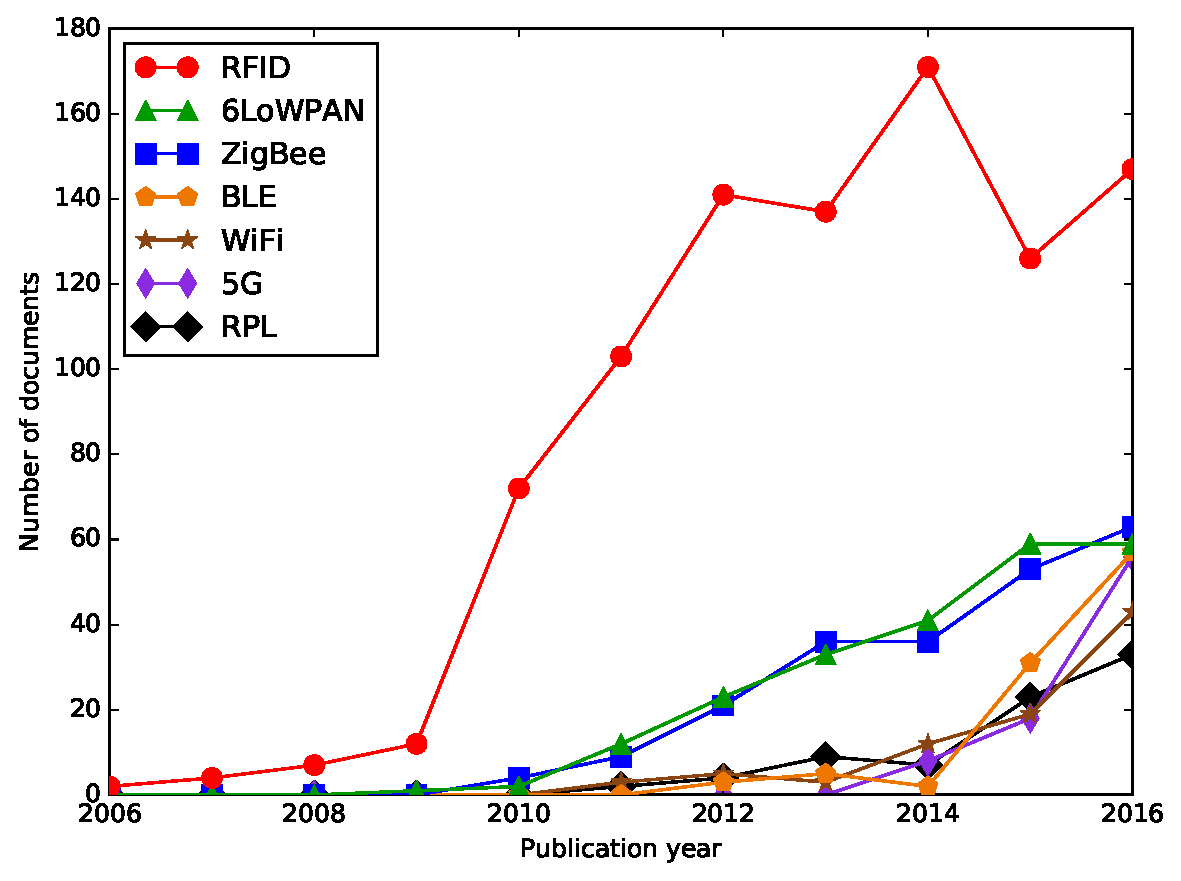
\includegraphics[width=\textwidth]{./graphs/figure6a.eps}
		\caption{}
		\label{fig_media_layers}
	\end{subfigure}
	\begin{subfigure}[b]{0.49\textwidth}
		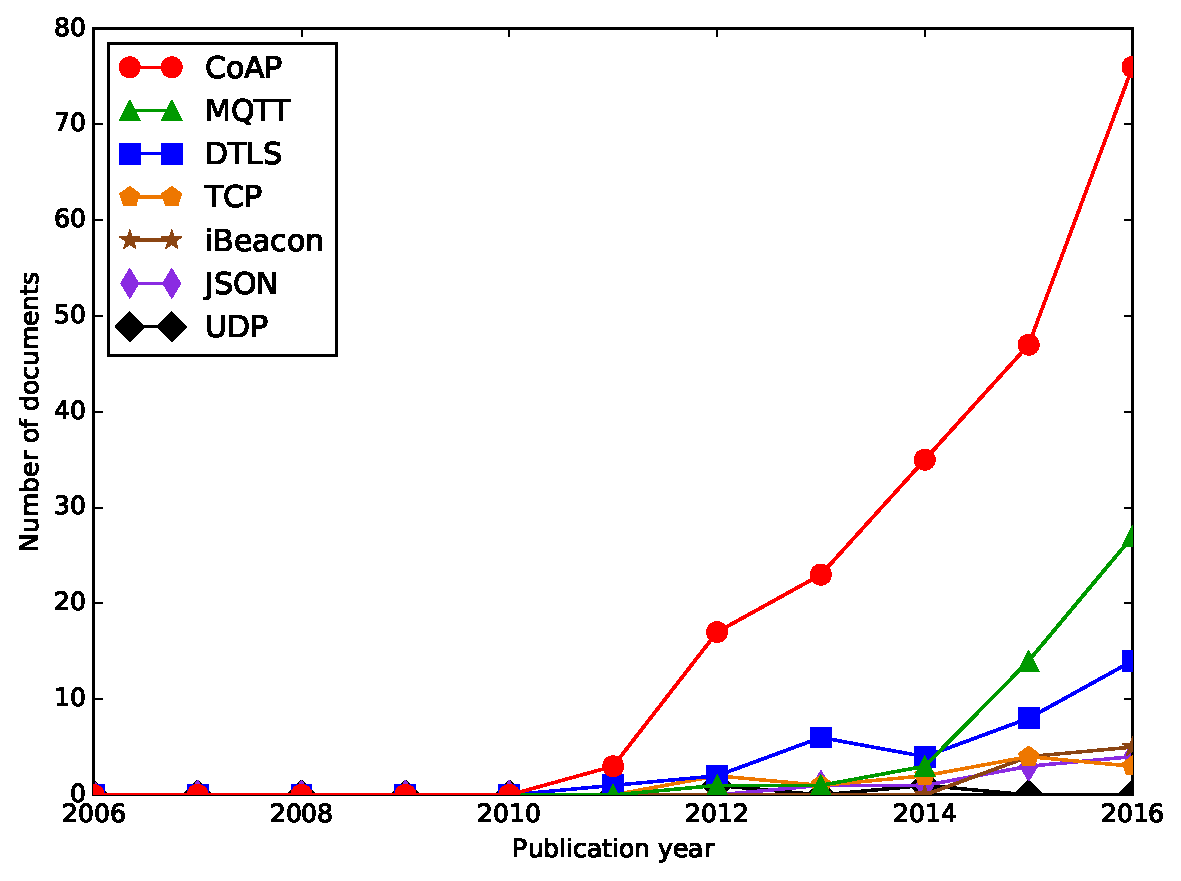
\includegraphics[width=\textwidth]{./graphs/figure6b.eps}
		\caption{}
		\label{fig_host_layers}
	\end{subfigure}
		\vspace{-12pt}
	\caption{Internet of Things media and host layers communication protocols based on authors' keywords in documents per year, for the 2006 to 2016 period.  (\textbf{a}) media layers' communications protocols (\textbf{b}) host layers' communication protocols.}
	\label{fig_comms_protocols}
\end{figure}

\noindent
\textcolor{brown}{To get the previous figure, run the following script for media layers' communications protocols:}\\
\begin{verbatim}
python scientoPy.py authorKeywords -t \
"RFID,RADIO FREQUENCY IDENTIFICATION;6LoWPAN;\
ZigBee;BLE,Bluetooth Low Energy;WiFi,Wi-Fi;5G;RPL" \
--startYear 2006 --savePlot "media_layers.eps"
\end{verbatim}

\noindent
\textcolor{brown}{To get the previous figure, run the following script for host layers' communication protocols:}\\
\begin{verbatim}
python scientoPy.py authorKeywords -t \
"CoAP,Constrained Application Protocol;MQTT,Message Queue Telemetry Transport;\
DTLS,Datagram Transport Layer Security;TCP;iBeacon;JSON;UDP" \
--startYear 2006 --savePlot "host_layers.eps"
\end{verbatim}



RFID is the top used author's keyword in the analyzed data set and the most used media layer communication protocol in the authors' research. On IoT 923 publications are related to RFID, where~security authentication \cite{Yuan2016,Li20124971,Li2016}, wireless sensors networks \cite{Hamza2016267,6322530}, privacy \cite{Wu20151224,Burmester2014317}, and electronic product code (ECP) \cite{Yan201255,Xu201140} were major applications. Next, 6LoWPAN appears in 230~publications, with~documents related to upper layer protocols such as Constrained Application Protocol (CoAP) \cite{Castellani201471,Bimschas2012}, Routing Protocol for Low power and Lossy Networks (RPL)~\cite{Pongle2015,Hellaoui201525}, and operating systems like Contiki \cite{Bragg20161273,Caputo2012770}, and Android \cite{Wang201549,Schleiss201214}. With similar growth, ZigBee follows with 222~documents, and research integrates this protocol with solutions such as RFID \cite{Fan2012732,Alharbe2013191,zhang2014}, or~applications like smart home \cite{Yiqi2014114,Yi2016128,wang2013}, and health care \cite{Kodali2016411,Spano20165452,Rosner201444}.

Bluetooth Low Energy (BLE) has experienced a rapid growth in the last three years, near 100\% from 2015 to 2016. A total of 98 documents on IoT are related to BLE, with one of the most cited articles by Gomez et al. at 176 citations. In this article, the authors describe the main features and potential applications for BLE technology \cite{Gomez201211734}. This data set shows BLE related applications such as home automation \cite{Horvat2016435,Pham-Huu201675,Papp2016366} and indoor location \cite{Kudeshia20161,Peng2017794,Vasilateanu2016} and health care \cite{Kang2016313,Touati20161271,Fafoutis20161}. WiFi is the other network protocol used for IoT research, with a total of 85 publications, and applications related to: home~automation \cite{Gao2016526,Airola2015111}, indoor localization \cite{Nambiar2017952}. Nevertheless, with this wireless technology, some~authors have focused on how the 2.4 GHz spectrum could be efficiently used with other IoT network protocols \cite{Zhang2012504,Samuel2016364,Rajandekar2015681,King201445,Lim2015,Shi2015204,Ndih20161835}. Similarly, 5th generation mobile networks (5G) appear in IoT with 82~publications, much more than 4G and LTE, with 54 documents both combined. The most cited paper is a suvery on 5G architecture and emerging technologies written by Gupta et al. \cite{Gupta20151206} with 109~citations. Network Function Visualization (NFV) and Software Defined Networking (SDN) \cite{Costa-Requena2015154,Uher2016,Kljaic2016587} were the top related technologies, which offer different architectural options to address IoT needs for 5G. Finally,~RPL~is discussed as an IPv6 Routing Protocol for Low-Power and Lossy Networks as a mechanism for multipoint-to-point and point-to-multipoint traffic for these kinds of networks \cite{rfc6550}. This protocol has 78 documents with publications related to the Contiki OS and its simulator tool Cooja for WSN \cite{GauthamKrishna2016270,Ancillotti20131275}, and mesh networks \cite{Vittecoq2013530,Duquennoy2015337,Sebastian2017127}.



At the host layer, communication protocols publications are led by the Constrained Application Protocol (CoAP), which is a specialized web transfer protocol for use with constrained nodes and constrained networks \cite{rfc7252}. A total of 201 publications were found in this area, with some of these publications related to: 6LoWPAN \cite{Bimschas2012,Hellaoui201525,Mohiuddin201424}, and  Datagram Transport Layer Security (DTLS) \cite{Bhattacharyya2015682,Lakkundi20147}. Second, the Message Queue Telemetry Transport (MQTT) shows up with 46 documents. This is a lightweight, and open client-server publish/subscribe messaging transport protocol \cite{hillar2017mqtt}. Next, Datagram Transport Layer Security (DTLS) protocol follows this list with 35 publications. This DTLS provides communications privacy for datagram protocols based on the stream-oriented Transport Layer Security (TLS) \cite{rfc6347}. This protocol helps to enhance the security of others' higher layers protocols like CoAP \cite{LessaDosSantos2016809,Raza20133711}. Finally, iBeacon is the fifth on this list with nine documents. This is a protocol designed by Apple (Cupertino, CA, United States) to describe its own implementation of BLE Beacon, which emits a signal that can be detected by any BLE enabled device within a close range \cite{Newman2014222}. Most of the applications for this protocol include indoor localization~\mbox{\cite{Yang2015161,Xiong2016}}.


\subsection{Software Processing Techniques}

The proliferation of IoT has significantly increased the data collection and the strain it places on faster data analytics. Several software processing techniques have been researched, developed, and published. In these published documents, the various software processing techniques used were specified in the authors' keywords. Figure \ref{fig_software_processing} shows the top authors' keywords for these processing techniques. Machine learning is the most popular research technique for data processing with 100~publications. This technique is used for data prediction \cite{Wu20162062,Han2016109}, activity recognition \cite{AlSafadi201673,7808003}, and data classification \cite{Khan201461,Keshan20152661}. Next, data mining appears with 89 documents, with distributed data mining \cite{Kholod2016480}, and applications such as event detection \cite{Bhuiyan2017109,Tseng2015} as sub-techniques.


\begin{figure}[H]
	\centering
	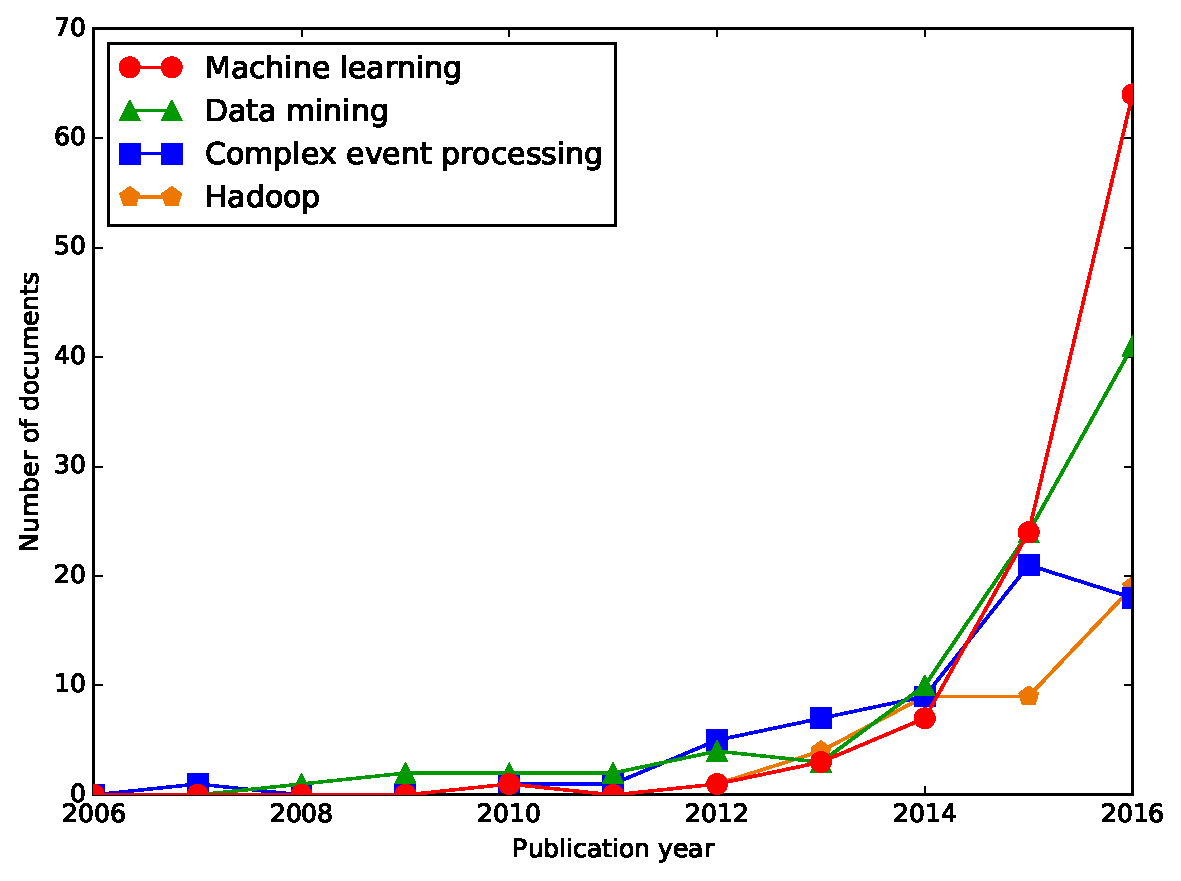
\includegraphics[width=\figuresWidth]{./graphs/figure7.eps}
	\caption{Internet of Things software processing techniques based on authors' keywords in documents per year, for the period 2006 to 2016.}
	\label{fig_software_processing}
\end{figure} 

\noindent
\textcolor{brown}{To get the previous figure, run the following script:}\\
\begin{verbatim}
python scientoPy.py authorKeywords -t \
"Machine learning;Data mining;Complex event processing,CEP;Hadoop" \
--startYear 2006 --savePlot "software.eps"
\end{verbatim}

Complex event processing is a method of tracking and analyzing streams of data surrounding events or anomalies and basing a conclusion from them \cite{Luckham:2001:PEI:515781}. It was found that 63 documents are related to this processing  technique with applications such as supply chain \cite{Li20131481,li2013,Liu2015} and health care \cite{Mohamedali201650,Sheriff2015}. Apache Hadoop (or Hadoop) is a software framework used for distributed storage and big data processing using the MapReduce programming model \cite{White:2009:HDG:1717298}, appearing with 42 documents and applications including smart cities \cite{Ji201422372,Hans2016352,TahmassebpourS1442}, and Social Internet of Things \cite{Ahmad20161101}.


\subsection{Device Operating Systems (OS) and Hardware}

The data set analyzed here shows that the investigations used different IoT devices (end devices and gateway devices), operating systems (OS), and hardware. Figure \ref{fig_os_hardware} shows the top authors' keywords per year for the most employed OS and hardware. Android is the most used OS for researchers, with 87 documents. This OS is used for IoT gateways \cite{Chen2015218,Bian2011526,Carlson2013619,Garcia201654} or end sensing devices~\mbox{\cite{Prakash2016,Sutar201673,Hossain20155095}}. Contiki is a lightweight OS for memory constrained systems (like microcontroller-based systems) designed for low-power wireless devices \cite{1367266}. A total of 56~publications were found related to this OS, where the author uses capabilities like embedded protocols: 6LoWPAN \cite{Bragg20161273,Anjana2016}, CoAP \cite{Yassein2016160}, and RPL \cite{Gonizzi20131400}. In addition, some publications use the Contiki network simulator Cooja to simulate routing protocols \cite{Banh2016206} and performance evaluation \cite{Sitanayah2013}.

\begin{figure}[H]
	\centering
	\begin{subfigure}[b]{0.49\textwidth}
		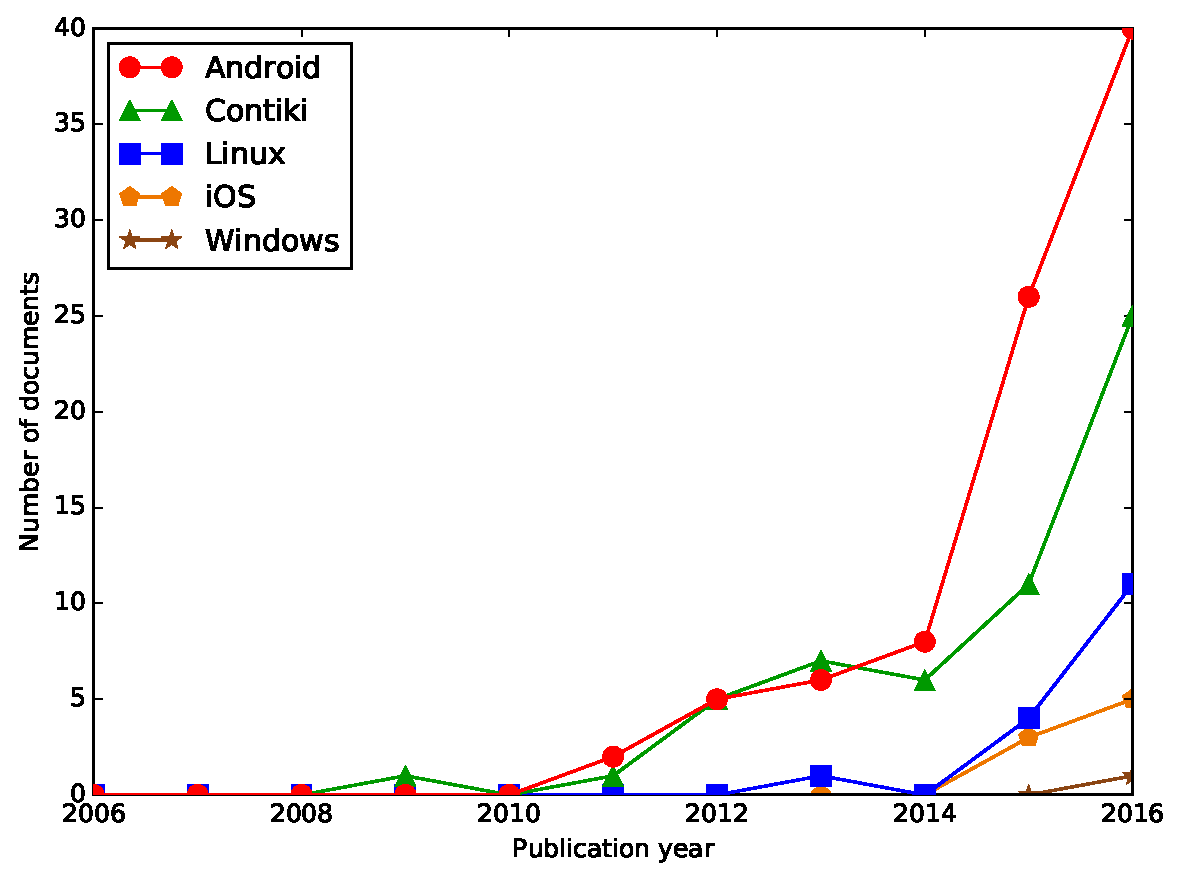
\includegraphics[width=\textwidth]{./graphs/figure8a.eps}
		\caption{}
		\label{fig_operating_systems}
	\end{subfigure}
	\begin{subfigure}[b]{0.49\textwidth}
		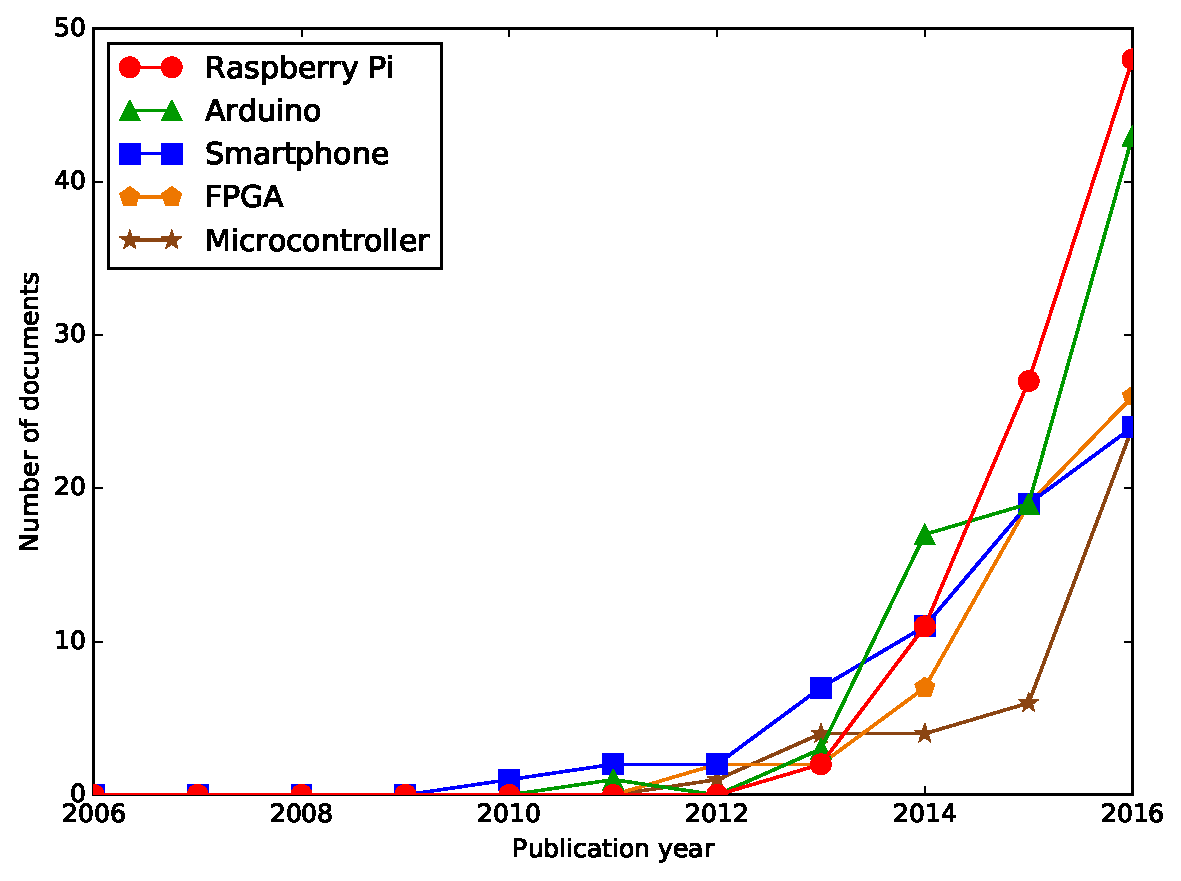
\includegraphics[width=\textwidth]{./graphs/figure8b.eps}
		\caption{}
		\label{fig_hardware}
	\end{subfigure}
			\vspace{-12pt}
	\caption{Internet of Things devices operating systems (OS) and hardware based on authors' keywords, for the period 2006 to 2016. (\textbf{a}) most used operating systems in authors' keywords per year; (\textbf{b}) most used hardware in authors' keywords per year.}
	\label{fig_os_hardware}
\end{figure}


\noindent
\textcolor{brown}{To get the previous figure, run the following script for operating systems:}\\
\begin{verbatim}
python scientoPy.py authorKeywords -t \
"Android,Android OS;Contiki,Contiki OS;Linux,Linux OS;\
iOS,iPhone Operating System,iPhone Operating System (iOS);\
Windows,Windows OS" --startYear 2006 --savePlot "operating.eps"
\end{verbatim}

\noindent
\textcolor{brown}{To get the previous figure, run the following script for hardware:}\\
\begin{verbatim}
python scientoPy.py authorKeywords -t \
"Raspberry Pi;Arduino,Arduino board;Smartphone,Smartphones,Smart phone,Smart phones;\
FPGA,Field-programmable gate array,Field programmable gate array;\
Microcontroller,Microcontrollers" --startYear 2006 --savePlot "hardware.eps"
\end{verbatim}

Other operating systems, such as Linux, are used in IoT for image processing \cite{Dinesh2016} and gateway services \cite{Xu20164713}. The iPhone Operating System (iOS) is used as user interface for presentation, configuration, and remote controlling for IoT environments \cite{Kovalcik2016}. Finally, last year, Culic et al. demonstrated the potential of Windows 10 IoT Core (Redmond, WA, United States), a light-weight version of Windows 10, as an IoT operating system optimized to run on small devices that have no display \cite{7753246}.

On the hardware side, some authors' keywords detail the hardware devices employed (see~Figure~\ref{fig_os_hardware}b). Raspberry Pi is a small single board computer (SBC) capable of supporting operating systems like Linux Ubuntu, Windows, or Android. The Raspberry Pi is the most popular platform employed for IoT, with 88 publications, as a versatile platform for a gateway \cite{Suresh201517163,Kim20171533,Gloria2017568} or monitoring system \cite{7380571,Balasubramaniyan2016}. Arduino boards are single-board microcontroller kits, in which the developer connects sensors, actuators, or RF communication interface easily using shield boards. For this specific IoT publications data set, 83 documents refer to Arduino hardware. These boards are widely used for IoT learning \cite{Bogdanovic2014259,Raikar201715,Kovalcik2016} and monitoring devices \cite{Amin201543663,Fuertes201658,Ashwini20164311}. 


Presently, smartphones are highly capable embedded systems that run full OS, with integrated sensors. Sixty-six documents were found related to smartphones in IoT, be they used as sensors \cite{Behringer2016179,Kothandaraman2016661}, gateway \cite{Seol2015133,Gupta2016416,Pereira2016}, or user interface \cite{Mayer201446,Lee20163777}. The Field-Programmable Gate Array (FPGA) is a hardware reconfigurable component that contains an array of computational (logic) elements, with~a functionality specified by a hardware description language \cite{Compton2002171}. These FPGAs are used in IoT investigations for data encryption \cite{Prasetyo201475,Rao20152212,Prathiba2016}, routing algorithms \cite{Qu2012124}, and parallel simulation \cite{Wehner2014}. A~microcontroller (MCU) is a small computer on a single integrated circuit, which includes a processor core, RAM/ROM memory, peripherals, and, in some cases, RF transceivers. For IoT, the MCU plays a fundamental role in sensing end devices \cite{Lee2016155,Suresh201517163,Lim201690} and actuators \cite{Sushmitha201619874}.


\subsection{Top Trending Topics}

For this analysis, the top trending topics are the authors' keywords, which have higher average growth rate (AGR) over the others. These topics represent concepts that have a large impact on IoT research. To find these trending topics, two-year AGR time periods (2011--2012, 2013--2014, and~2015--2016) were found using the following Equation \eqref{equation_AGR}:
\begin{equation}
AGR = \frac{\sum\limits_{i = Y_s}^{Y_e}P_i - P_{i-1}}{(Y_e - Y_s)+1},  
\label{equation_AGR}
\end{equation}
where:

%\hspace*{3em}
%\begin{tabular}{rcl}
$AGR$ = Average growth rate;
	
	$Y_s$ = Start year;
	
	$Y_e$ = End year;
	
	$P_i$ = Number of publications on year $i.$
%\end{tabular}
\newline

Figure \ref{fig_trending} shows the top eight trending topics with the AGR time periods. Cloud computing leads, with an AGR of 90 publications/year for 2015--2016, 284 documents on 2016, and a constant growth in all time periods. In 2013, Gubbi et al. mentioned that the integration of IoT with Cloud computing applications can enable the creation of smart environments such as Smart Cities and others \cite{Gubbi20131645}. The~growth of publications about IoT related to Cloud computing shows that the mentioned integration is currently happening. The second trending topic on this list is security. This topic has a moderate growth in 2011--2012 and 2013--2014 periods (about 18 publications/years), but, in 2015--2016, its growth soared to 83 publications/year. Security backs the industry's concerns about the user privacy and confidentiality \cite{Zhang2018,Suo2012648}. The same way that the communications protocols were analyzed in this paper by layers, Jing et al. divided the IoT into three layers (perception, transportation, and~application layers) to analyze features and security issues of each \cite{Jing2014}.

\begin{figure}[H]
	\centering
	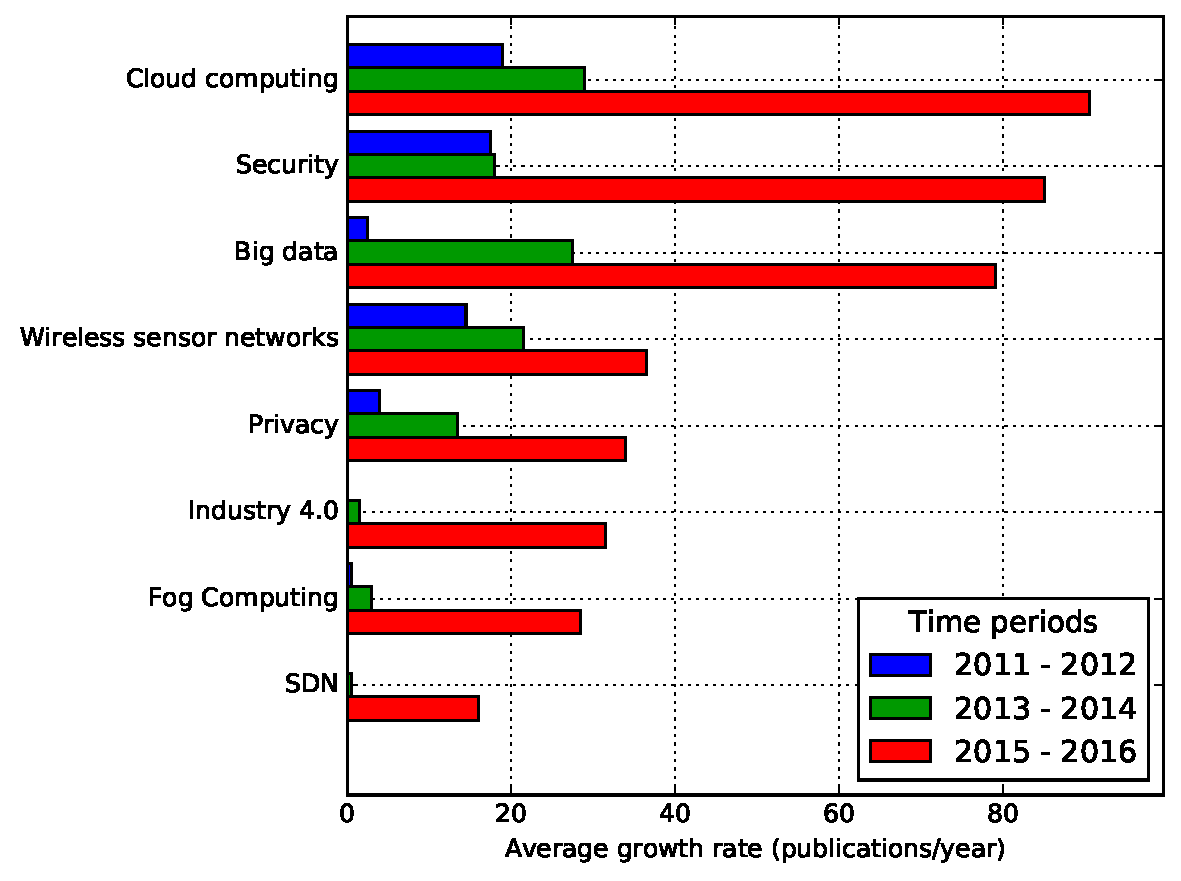
\includegraphics[width=0.8\textwidth]{./graphs/figure9.eps}
	\caption{Internet of Things top trending topics based on authors' keywords, with average growth rate (AGR) for different times periods (2011--2012, 2013--2014, and 2015--2016).}
	\label{fig_trending}
\end{figure} 

\noindent
\textcolor{brown}{To get the previous figure, run the following script for hardware:}\\
\begin{verbatim}
python trendResults.py authorKeywords -t \
"Cloud computing;Security;Big Data;Wireless sensor networks;\
Privacy;Industry 4.0;Fog computing;SDN" --savePlot "trending.eps"
\end{verbatim}


IoT is one of many applications of Big Data because the rapid growth of IoT devices further propels the sharp growth of data to be processed and analyzed \cite{Chen2014171}. Wireless sensors networks (WSN), such as RFID, is one of the most important technologies enabling the IoT \cite{ROMAN2011147}. Likewise,~security/privacy is a trending topic and also a concern in IoT, which was well summarized in \cite{Ziegeldorf20142728}.

Industry 4.0 is a new trending topic, without any growth in the 2011--2012 period, but with a sharp rise in publications from 3 to 66 in 2014 to 2016. Industry 4.0 includes the use of intelligent manufacturing processes, Cyber-Physical Systems (CPSs), and implementation and operation of smart factories \cite{7382284}. This fourth industrial revolution aims to integrate IoT technologies such as remote control, manufacturing analytic tools and services, supply chains integration, and tracking and tracing inter- and intra-plant logistics \cite{Weinberger2016699}. Fog computing is also a new trending topic, with a small growth in 2011--2014 periods, but a large increase in the 2015--2016 period. Fog is a platform that provides compute, storage and networking services between end devices and cloud computing servers, most~commonly, but not exclusively, located at the edge of network \cite{Bonomi201213}. For IoT, this new platform is aimed to decentralize the data processing \cite{Gonzalez2017}, decrease the latency \cite{7548853}, and bring more reliability for WSN~\cite{6623445}. Finally, Software-Defined Networking (SDN) is a novel concept for IoT, without any growth in the 2011--2012 period, but which was gaining popularity from one publication in 2013, and 2014, to 33 in 2016. SDN brings network routing intelligence via a centralized controller that connects to the network switch through the OpenFlow protocol \cite{Flauzac2015688}, for example. This allows efficient node mobility \cite{Oh2016}, resource management \cite{7365931}, and improves the security of IoT networks \cite{Vilalta2016,Flauzac2015688,Hafeez201655}.


\section{Conclusions}

A scientometrics review about Internet of Things was performed over a data set of 19,035~documents published during a period of 15 years (2002--2016) from two databases (Clarivate~Web of Science and Scopus). A Python script called ScientoPy was developed to make a quantitative analysis of this data set, providing insight into research trends by investigating primary author's country affiliation, most published authors, and prevalence of various research topics. Using authors' keywords, the top research topics for IoT were found, including applications, communication protocols, software processing, hardware, and operating systems.  

Analysis by country affiliation of the primary author shows a major increase in the number of publications for IoT in countries where the government has possibly implemented polices that improve the development of IoT. Similarly, this increase has shown in countries where private initiatives could have launched commercial low cost IoT networks (such as LoRa, Sigfox, etc.). In addition,~prototype~IoT infrastructure on small test environments, such as universities, creates microcosms that foster investigations for different IoT applications. 

From 2014 to 2016, there was a sharp growth of smart environments including smart city, home, grids, and other surfaces with technology incorporating Big Data and cloud computing into IoT devices. Nevertheless, security \cite{UlRehman2016,Alohali2014115,Peter2017} and privacy  \cite{Beligianni2016,Winter201545,Dalipi201663} are major concerns for many applications such as smart home and grid. Cyber-Physical Systems is an application that, when powered by the IoT, enables the targets fixed by Industry 4.0 \cite{Zhou2016167}. Trends in communications protocols have changed in the last few years. The RFID publications sigmoid growth is on a stationary phase, while other media layer protocols such as BLE, WiFi, and 5G are on sigmoid growth exponential phase. Host layer protocols show a high growth rate for CoAP and MQTT. Software data processing demonstrates that the techniques designed to work with Big Data are growing on the sigmoid exponential phase for IoT data processing environments.  

For operating systems, Android has become the most used OS for scientific researchers on IoT. This~OS has been used for IoT gateways \cite{Chen2015218,Bian2011526,Carlson2013619,Garcia201654} and user interface in IoT devices \cite{Mayer201446,Lee20163777}. Contiki~is growing in a sigmoid exponential phase with its integrated protocol stack and WSN simulator, Cooja. Similarly, in IoT research, Raspberry Pi and Arduino are the most popular platforms for learning and development. In addition, the combination is widely used wherein Raspberry Pi is an IoT gateway \cite{Suresh201517163,Kim20171533,Gloria2017568} and Arduino boards serve as edge monitoring devices \cite{Amin201543663,Fuertes201658,Ashwini20164311}. Similarly, smartphones exhibit their versatility being used as gateway  \cite{Seol2015133,Gupta2016416,Pereira2016}, user interface \cite{Mayer201446,Lee20163777}, and sensing \cite{Behringer2016179,Kothandaraman2016661} IoT devices. Meanwhile, FPGAs have exhibited a sigmoid exponential phase growth in the last two years, with applications such as data encryption \cite{Prasetyo201475,Rao20152212,Prathiba2016}, routing algorithms optimization \cite{Qu2012124}, and parallel networks simulation \cite{Wehner2014}. 

Top trending topics demonstrate that cloud integration with IoT devices is enabling the implementation of smart environments. Nevertheless, security and privacy in these environments are important growing concerns for IoT researchers and industry. WSNs are one of the most utilized technologies enabling the IoT. Furthermore, Fog computing has emerged as a promising edge device to decentralize data processing, decrease latency, and bring more reliability for WSN in IoT. Likewise,~research~on Software Defined Networks (SDN) grew rapidly during the last year, offering~more efficient nodes, mobility, resources management, and improved security of IoT networks. The related trending topics offer unique opportunities for IoT innovations and start-ups in pursuit of an efficient, secure, and reliable IoT environment. 

\vspace{6pt}

\acknowledgments{This research is funded by Colciencias Doctoral scholarship 647-2014 for the PhD in Telematic Engineering at the Universidad del Cauca, Popayán, Colombia.}

\authorcontributions{Juan Ruiz-Rosero, Gustavo Ramirez-Gonzalez, and Rahul Khanna proposed the concept of this research. Jennifer M. Williams and Huaping Liu contributed for the state of art and final paper draft revisions. Greeshma Pisharody and Rahul Kahanna contributed to analize the data and to revise the drafts of the paper. Juan Ruiz-Rosero and Gustavo Ramirez-Gonzalez desiged, build, and validate the ScientoPy script. Juan Ruiz-Rosero, Gustavo Ramirez-Gonzalez, Rahul Khanna and Jennifer M. Williams wrote the paper.}

%For manuscripts with more than one author, please state individual contributions of each author to research and writing of the manuscript.
\conflictsofinterest{The authors declare no conflict of interest.}
%Please disclose conflicts of interest, or add 'The authors declare no conflicts of interest'. 


%%%%%%%%%%%%%%%%%%%%%%%%%%%%%%%%%%%%%%%%%%
% Citations and References in Supplementary files are permitted provided that they also appear in the reference list here. 

%=====================================
% References, variant A: internal bibliography
%=====================================
\reftitle{References}
\begin{thebibliography}{999}

\bibitem[Williams \em{et~al.}(2017)Williams, Khanna, Ruiz-Rosero, Pisharody,
Qian, Carlson, Liu, and Ramirez-Gonzalez]{8064227}
Williams, J.M.; Khanna, R.; Ruiz-Rosero, J.P.; Pisharody, G.; Qian, Y.;
Carlson, C.R.; Liu, H.; Ramirez-Gonzalez,~G.
\newblock Weaving the Wireless Web: Toward a Low-Power, Dense Wireless Sensor
Network for the Industrial IoT.
\newblock {\em IEEE Microw. Mag.} {\bf 2017}, {\em 18},~40--63.

\bibitem[Hiremath \em{et~al.}(2015)Hiremath, Yang, and
Mankodiya]{Hiremath2015304}
Hiremath, S.; Yang, G.; Mankodiya, K.
\newblock \emph{Wearable Internet of Things: Concept, Architectural Components and
	Promises for Person-Centered Healthcare};
\newblock Institute of Electrical and Electronics Engineers Inc.: Piscataway, NJ, USA, 2015; pp.
304--307.

\bibitem[Williams \em{et~al.}(2017)Williams, Ruiz-Rosero, Ramirez-Gonzalez,
Khanna, , Pisharody, Qian, Wang, Carlson, and Liu]{Williams2017a}
Williams, J.M.; Ruiz-Rosero, J.P.; Ramirez-Gonzalez, G.; Khanna, R.;
Pisharody, G.; Qian, Y.; Wang, J.; Carlson,~C.R.; Liu, H.
\newblock \emph{Enabling Densely-Scalable Low-Power WSNs for Shipping and Industrial
	IoT};
\newblock Institute of Electrical and Electronics Engineers Inc.: Piscataway, NJ, USA, 2017.

\bibitem[Gerla \em{et~al.}(2014)Gerla, Lee, Pau, and Lee]{Gerla2014241}
Gerla, M.; Lee, E.K.; Pau, G.; Lee, U.
\newblock \emph{Internet of Vehicles: From Intelligent Grid to Autonomous Cars and
	Vehicular Clouds};
\newblock {IEEE Computer Society: Washington, DC, USA, 2014}; pp. 241--246.

\bibitem[Bi \em{et~al.}(2014)Bi, Xu, and Wang]{Bi20141537}
Bi, Z.; Xu, L.; Wang, C.
\newblock Internet of Things for enterprise systems of modern manufacturing.
\newblock {\em IEEE Trans. Ind. Inf.} {\bf 2014}, {\em
	10},~1537--1546.

\bibitem[Spanò \em{et~al.}(2015)Spanò, Niccolini, Pascoli, and
Iannaccone]{Spano2015468}
Spanò, E.; Niccolini, L.; Pascoli, S.; Iannaccone, G.
\newblock Last-meter smart grid embedded in an internet-of-things platform.
\newblock {\em IEEE Trans. Smart Grid} {\bf 2015}, {\em 6},~468--476.

\bibitem[IBM(IBM Institute for Business Value, IBM Corporation, 2015)]{ibm2015}
IBM.
\newblock Redefining Boundaries: Insights from the Global C-Suite Study,  IBM
Institute for Business Value, IBM Corporation, 2015.
\newblock Available online: \url{https://public.dhe.ibm.com/common/ssi/ecm/gb/en/gbe03695usen/GBE03695USEN.PDF
} (accessed on 28 August 2017).

\bibitem[Garcia-Sanchez \em{et~al.}(2011)Garcia-Sanchez, Garcia-Sanchez, and
Garcia-Haro]{GARCIASANCHEZ2011288}
Garcia-Sanchez, A.J.; Garcia-Sanchez, F.; Garcia-Haro, J.
\newblock wireless sensor network deployment for integrating video-surveillance
and data-monitoring in precision agriculture over distributed crops.
\newblock {\em Comput. Electron. Agric.} {\bf 2011}, {\em
	75},~288--303.

\bibitem[Buratti \em{et~al.}(2016)Buratti, Stajkic, Gardasevic, Milardo,
Abrignani, Mijovic, Morabito, and Verdone]{7172291}
Buratti, C.; Stajkic, A.; Gardasevic, G.; Milardo, S.; Abrignani, M.D.;
Mijovic, S.; Morabito, G.; Verdone, R.
\newblock Testing Protocols for the Internet of Things on the EuWIn Platform.
\newblock {\em IEEE Int. Things J.} {\bf 2016}, {\em 3},~124--133.

\bibitem[Ruiz-Rosero and Ramirez-Gonzalez(2014)]{ruiz2014firmware}
Ruiz-Rosero, J.; Ramirez-Gonzalez, G.
\newblock Firmware architecture to support Plug and Play sensors for IoT
environment. In Proceedings of the VII Congreso Iberoamericano de Telemática CITA 2015, Popayán, Colombia,
\newblock 10--12 June 2015.

\bibitem[Khanna \em{et~al.}(2014)Khanna, Liu, and Rangarajan]{6957004}
Khanna, R.; Liu, H.; Rangarajan, T.
\newblock Wireless Data Center Management: Sensor Network Applications and
Challenges.
\newblock {\em IEEE Microw. Mag.} {\bf 2014}, {\em 15},~S45--S60.

\bibitem[Atzori \em{et~al.}(2010)Atzori, Iera, and Morabito]{Atzori20102787}
Atzori, L.; Iera, A.; Morabito, G.
\newblock The Internet of Things: A survey.
\newblock {\em Comput. Netw.} {\bf 2010}, {\em 54},~2787--2805.

\bibitem[Gubbi \em{et~al.}(2013)Gubbi, Buyya, Marusic, and
Palaniswami]{Gubbi20131645}
Gubbi, J.; Buyya, R.; Marusic, S.; Palaniswami, M.
\newblock Internet of Things (IoT): A vision, architectural elements, and
future directions.
\newblock {\em Future Gener. Comput. Syst.} {\bf 2013}, {\em
	29},~1645--1660.

\bibitem[Borgia(2014)]{Borgia20141}
Borgia, E.
\newblock The internet of things vision: Key features, applications and open
issues.
\newblock {\em Comput. Commun.} {\bf 2014},~{\em 54},~1--31.

\bibitem[Yan \em{et~al.}(2015)Yan, Lee, and Lee]{Yan2015}
Yan, B.N.; Lee, T.S.; Lee, T.P.
\newblock Mapping the intellectual structure of the Internet of Things (IoT)
field (2000--2014): A co-word analysis.
\newblock {\em Scientometrics} {\bf 2015}, {\em 105},~1285--1300.

\bibitem[Mishra \em{et~al.}(2016)Mishra, Gunasekaran, Childe, Papadopoulos,
Dubey, and Wamba]{Mishra20161331}
Mishra, D.; Gunasekaran, A.; Childe, S.; Papadopoulos, T.; Dubey, R.; Wamba, S.
\newblock Vision, applications and future challenges of Internet of Things: A
bibliometric study of the recent literature.
\newblock {\em Ind. Manag. Data Syst.} {\bf 2016}, {\em
	116},~1331--1355.

\bibitem[Leydesdorff and Milojevic(2012)]{DBLP:journals/corr/abs-1208-4566}
Leydesdorff, L.; Milojevic, S.
\newblock Scientometrics.
\newblock {\em arXiv} {\bf 2012},  arXiv:1208.4566v2.

\bibitem[Schoenberger({2002})]{ISI:000174207300032}
Schoenberger, C.
\newblock {The Internet of Things}.
\newblock {\em {FORBES}} {\bf {2002}}, {\em {169}},

\bibitem[Qiu and Zhang(2003)]{Qiu20032661}
Qiu, R.; Zhang, Z.
\newblock Design of enterprise web servers in support of instant information
retrievals.
\newblock In~Proceedings of the IEEE International Conference on Systems, Man and Cybernetics, Washington, DC, USA, 8 October 2003; Volume~3, pp. 2661--2666.

\bibitem[Traversat \em{et~al.}(2003)Traversat, Abdelaziz, Doolin, Duigou,
Hugly, and Pouyoul]{Traversat2003}
Traversat, B.; Abdelaziz, M.; Doolin, D.; Duigou, M.; Hugly, J.C.; Pouyoul, E.
\newblock {Project JXTA-C: Enabling a Web of Things}.
\newblock 2003.
\newblock cited By 23. Available online: \url{http://ieeexplore.ieee.org/document/1174816/} (accessed on 10 August 2017). 

\bibitem[Gershenfeld \em{et~al.}(2004)Gershenfeld, Krikorian, and
Cohen]{Gershenfeld200476}
Gershenfeld, N.; Krikorian, R.; Cohen, D.
\newblock The internet of things.
\newblock {\em Sci. Am.} {\bf 2004}, {\em 291},~76--81.

\bibitem[Luckett({2004})]{ISI:000224027400006}
Luckett, D.
\newblock {The supply chain}.
\newblock {\em {BT Technol. J.}} {\bf {2004}}, {\em {22}},~{50--55}.

\bibitem[Böse and Lampe(2005)]{Bose2005}
Böse, F.; Lampe, W.
\newblock {Adoption of RFID in logistics}.
\newblock \emph{IBIMA} \textbf{2005}, \emph{1} 62-65.

\bibitem[Norman(2005)]{Norman2005}
Norman, A.
\newblock \emph{Leveraging Radio Frequency Identification (RFID) Technology for Halal
	Tracking Tag}; Universiti Malaya: Kuala Lumpur, Malaysia,
\newblock 2005; Volume~1.

\bibitem[Djassemi and Singh(2005)]{Djassemi2005}
Djassemi, M.; Singh, J.
\newblock The use of RFID in manufacturing and packaging technology
laboratories. In~Proceedings of the Thirty-Third North American Manufacturing Research Conference,
\newblock New York, NY, USA, 23--27 May 2005; Volume TP05PUB223.

\bibitem[Pujolle(2006)]{4022056}
Pujolle, G.
\newblock An Autonomic-oriented Architecture for the Internet of Things.
\newblock In Proceedings of the IEEE John Vincent Atanasoff 2006 International Symposium on Modern
Computing (JVA'06), Sofia, Bulgaria, 3--6~October~2006; pp. 163--168.

\bibitem[Bernard(2006)]{1698342}
Bernard, G.
\newblock Invited Paper: Middleware for Next Generation Distributed Systems:
Main Challenges and Perspectives.
\newblock In Proceedings of the 17th International Workshop on Database and Expert Systems
Applications (DEXA'06), Krakow, Poland, 4--8 September 2006; pp. 237--240.

\bibitem[Adelmann \em{et~al.}(2006)Adelmann, Langheinrich, and
Flörkemeier]{Adelmann2006366}
Adelmann, R.; Langheinrich, M.; Flörkemeier, C.
\newblock To Olkit for Bar Code Recognition and Resolving on Camera Phones---Jump Starting the Internet of Things.
\newblock INFORMATIK \textbf{2006}, \emph{2}, 366--373.

\bibitem[Lehtonen \em{et~al.}(2006)Lehtonen, Michahelles, Staake, and
Fleisch]{Lehtonen200677}
Lehtonen, M.; Michahelles, F.; Staake, T.; Fleisch, E.
\newblock \emph{Strengthening the Security of Machine Readable Documents by Combining
	RFID and Optical Memory Devices};
\newblock Springer-Verlag: Paris, France, 2006; pp. 77--92.

\bibitem[Futatsumori \em{et~al.}(2006)Futatsumori, Kono, Hikage, Nojima, and
Koike]{Futatsumori2006258}
Futatsumori, S.; Kono, T.; Hikage, T.; Nojima, T.; Koike, B.
\newblock Experimental Test System to Assess the EMI From RFID Reader/writer On
Implantable Cardiac Pacemaker.
\newblock 2006, pp. 258--261. Available online: \url{https://www.scopus.com/record/display.uri?eid=2-s2.0-84901711947&origin=inward} (accessed on 10 August 2017)

\bibitem[Broll \em{et~al.}(2009)Broll, Rukzio, Paolucci, Wagner, Schmidt, and
Hussmann]{5262929}
Broll, G.; Rukzio, E.; Paolucci, M.; Wagner, M.; Schmidt, A.; Hussmann, H.
\newblock Perci: Pervasive Service Interaction with the Internet of Things.
\newblock {\em IEEE Int. Comput.} {\bf 2009}, {\em 13},~74--81.

\bibitem[Hvistendahl({2012})]{ISI:000304905300012}
Hvistendahl, M.
\newblock {Information Technology China Pushes the `Internet of Things'}.
\newblock {\em {Science}} {\bf {2012}}, {\em {336}},~{1223}.

\bibitem[Zhu \em{et~al.}(2010)Zhu, Wang, Chen, Liu, and Qin]{Zhu2010347}
Zhu, Q.; Wang, R.; Chen, Q.; Liu, Y.; Qin, W.
\newblock IOT gateway: Bridging wireless sensor networks into Internet of
Things. In Proceedings of the 2010 IEEE/IFIP 8th International Conference on Embedded and Ubiquitous Computing (EUC), Hong Kong, China, 11--13 December
\newblock 2010; pp. 347--352.

\bibitem[{The Economic Times}(2017)]{theEconomicTimes2017}
{The Economic Times}.
\newblock Internet of Things to Grow Rapidly in India by 2020: Report, 2017.
\newblock Available online: \url{http://economictimes.indiatimes.com/articleshow/57129635.cms} (accessed on 28 July 2017).

\bibitem[BBC(2016)]{bbcKorea2016}
BBC.
\newblock South Korea Launches First Internet of Things Network, 2016.
\newblock Available online: \url{http://www.bbc.com/news/technology-36710667} (accessed on 25~July~2017).

\bibitem[Estopace(2017)]{Estopace2017}
Estopace, E.
\newblock IDC Sees Gov’t Use of IoT in Indonesia by 2019, 2017.
\newblock Available online: \url{https://www.enterpriseinnovation.net/article/idc-sees-govt-use-iot-indonesia-2019-1967761722} (accessed on 25~July~2017).

\bibitem[{Telecompaper}(2017)]{turkey2017}
{Telecompaper}.
\newblock Xeelas, Sade to Build IoT Network in Turkey, 2017.
\newblock Available online: 
\url{https://www.telecompaper.com/news/xeelas-sade-to-build-iot-network-in-turkey--1189559} (accessed on 25 July 2017).

\bibitem[{Research an markets}(2017)]{russia2017}
{Research an Markets}.
\newblock Russia Internet of Things (IoT) Market Size, Demand, Opportunity \&
Growth Outlook 2023, 2017.
\newblock Available online: \url{https://www.researchandmarkets.com/research/xmn4pm/russia_internet} (accessed on 25 July 2017).

\bibitem[{Ignite National Technology Fund}(2017)]{ignite2017}
{Ignite National Technology Fund}.
\newblock Internet Of Things: It’s Happening!, 2017.
\newblock Available online:
\url{https://www.ictrdf.org.pk/blog/2017/01/23/internet-of-things-its-happening-2/} (accessed on 25 July 2017).

\bibitem[Yu \em{et~al.}({2013})Yu, Zhang, Gjessing, Xia, and
Yang]{ISI:000325658900009}
Yu, R.; Zhang, Y.; Gjessing, S.; Xia, W.; Yang, K.
\newblock {Toward Cloud-Based Vehicular Networks with Efficient Resource
	Management}.
\newblock {\em {IEEE Netw.}} {\bf {2013}}, {\em {27}},~{48--55}.

\bibitem[Li \em{et~al.}(2012)Li, Hou, Liu, and Liu]{Li2012}
Li, Y.; Hou, M.; Liu, H.; Liu, Y.
\newblock Towards a theoretical framework of strategic decision, supporting
capability and information sharing under the context of Internet of Things.
\newblock {\em Inf. Technol. Manag.} {\bf 2012}, {\em
	13},~205--216.

\bibitem[Wang \em{et~al.}(2014)Wang, Mao, and Nelms]{6737280}
Wang, Y.; Mao, S.; Nelms, R.M.
\newblock Distributed Online Algorithm for Optimal Real-Time Energy
Distribution in the Smart Grid.
\newblock {\em IEEE Int. Things J.} {\bf 2014}, {\em 1},~70--80.

\bibitem[Su \em{et~al.}(2011)Su, Li, and Fu]{Su20111028}
Su, K.; Li, J.; Fu, H.
\newblock Smart city and the applications. In Proceedings of the 2011 International Conference on Electronics, Communications and Control (ICECC), Ningbo, China, 9--11~September~2011;
\newblock  pp. 1028--1031.

\bibitem[Zhang \em{et~al.}(2013)Zhang, Iannucci, Hennessy, Gopal, Xiao, Kumar,
Pfeffer, Aljedia, Ren, Griss, Rosenberg, Cao, and Rowe]{6649727} % r45
Zhang, J.; Iannucci, B.; Hennessy, M.; Gopal, K.; Xiao, S.; Kumar, S.; Pfeffer,
D.; Aljedia, B.; Ren, Y.; Griss, M.; et al.
\newblock Sensor Data as a Service---A Federated Platform for Mobile
Data-centric Service Development and Sharing.
\newblock In Proceedings of the 2013 IEEE International Conference on Services Computing, Santa Clara, CA, USA, 28 June--3 July 2013; pp.
446--453.

\bibitem[Wang and Katabi(2013)]{Wang201351} % r46
Wang, J.; Katabi, D.
\newblock Dude, where's my card? RFID positioning that works with multipath and
non-line of sight. In Proceedings of the ACM SIGCOMM 2013 Conference on SIGCOMM,
\newblock Hong Kong, China, 12--16 August 2013; pp. 51--62.

\bibitem[Li \em{et~al.}(2010)Li, Zhang, Wang, Tao, Cao, Jiang, Song, and
Chai]{Li2010} % r47
Li, B.H.; Zhang, L.; Wang, S.L.; Tao, F.; Cao, J.W.; Jiang, X.D.; Song, X.;
Chai, X.D.
\newblock Cloud manufacturing: A~new service-oriented networked manufacturing
model.
\newblock {\em Comput. Integr. Manuf.
	Syst.} {\bf 2010}, {\em 16},~1--7.

\bibitem[Li \em{et~al.}(2013)Li, Zhong, Wang, and Cao]{Li20131696}
Li, W.; Zhong, Y.; Wang, X.; Cao, Y. % r48
\newblock Resource virtualization and service selection in cloud logistics.
\newblock {\em J. Netw. Comput. Appl.} {\bf 2013}, {\em
	36},~1696--1704.

\bibitem[Chen \em{et~al.}(2014)Chen, Han, Yang, Ma, Han, Jiang, Lai, Claffey,
Safar, and Liu]{Chen201481} % r49
Chen, Y.; Han, F.; Yang, Y.H.; Ma, H.; Han, Y.; Jiang, C.; Lai, H.Q.; Claffey,
D.; Safar, Z.; Liu, K.
\newblock Time-reversal wireless paradigm for green internet of things: An
overview.
\newblock {\em IEEE Int. Things J.} {\bf 2014}, {\em 1},~81--98.

\bibitem[Jara \em{et~al.}({2011})Jara, Zamora, and
Skarmeta]{ISI:000288757900012} % r50
Jara, A.J.; Zamora, M.A.; Skarmeta, A.F.G.
\newblock {An internet of things-based personal device for diabetes therapy
	management in ambient assisted living (AAL)}.
\newblock {\em {Pers. Ubiquitous Comput.}} {\bf {2011}}, {\em
	{15}},~{431--440}.

\bibitem[Yang \em{et~al.}(2015)Yang, Wang, and Zhang]{Yang2015161}
Yang, J.; Wang, Z.; Zhang, X. % r51
\newblock An iBeacon-based indoor positioning systems for hospitals.
\newblock {\em Int. J. Smart Home} {\bf 2015}, {\em
	9},~161--168.

\bibitem[Li \em{et~al.}(2015)Li, Gao, Chen, Zhao, Huang, Ye, Liu, Liu, and
Kang]{Li2015} % r52
Li, H.; Gao, B.; Chen, Z.; Zhao, Y.; Huang, P.; Ye, H.; Liu, L.; Liu, X.; Kang,
J.
\newblock A learnable parallel processing architecture towards unity of memory
and computing.
\newblock {\em Sci. Rep.} {\bf 2015}, {\em 5}, doi:10.1038/srep13330.

\bibitem[Qin \em{et~al.}(2016)Qin, Sheng, Falkner, Dustdar, Wang, and
Vasilakos]{Qin2016137} % r53
Qin, Y.; Sheng, Q.; Falkner, N.; Dustdar, S.; Wang, H.; Vasilakos, A.
\newblock When things matter: A survey on data-centric internet of things.
\newblock {\em J. Netw. Comput. Appl.} {\bf 2016}, {\em
	64},~137--153.

\bibitem[Li \em{et~al.}(2011)Li, Lu, Liang, Shen, Chen, and Lin]{Li201168}
Li, X.; Lu, R.; Liang, X.; Shen, X.; Chen, J.; Lin, X. % r54
\newblock Smart community: An internet of things application.
\newblock {\em IEEE~Commun. Mag.} {\bf 2011}, {\em 49},~68--75.

\bibitem[Sun \em{et~al.}(2010)Sun, Liu, Li, Fan, and Sun]{Sun20101}
Sun, Q.B.; Liu, J.; Li, S.; Fan, C.X.; Sun, J.J. % r55
\newblock Internet of Things: Summarize on concepts, architecture and key
technology problem.
\newblock {\em J. Beijing Univ.
	Posts Telecommun.} {\bf 2010}, {\em 33},~1--9.

\bibitem[Lim \em{et~al.}(2015)Lim, Son, Kim, Lee, Song, Choi, Lee, Kim, Lee,
Hyeon, and Kim]{Lim2015375} % r56
Lim, S.; Son, D.; Kim, J.; Lee, Y.; Song, J.K.; Choi, S.; Lee, D.; Kim, J.;
Lee, M.; Hyeon, T.; Kim,~D.H.
\newblock Transparent and stretchable interactive human machine interface based
on patterned graphene heterostructures.
\newblock {\em Adv.~Funct. Mater.} {\bf 2015}, {\em 25},~375--383.

\bibitem[Guo \em{et~al.}(2013)Guo, Zhang, Wang, Yu, and Zhou]{Guo20131531}
Guo, B.; Zhang, D.; Wang, Z.; Yu, Z.; Zhou, X. % r57
\newblock Opportunistic IoT: Exploring the harmonious interaction between human
and the internet of things.
\newblock {\em J. Netw. Comput. Appl.} {\bf 2013}, {\em
	36},~1531--1539.

\bibitem[Li and Liu(2013)]{Li20131147}
Li, J.; Liu, X. % r58
\newblock An important aspect of big data: Data usability.
\newblock {\em Comput. Res. Dev.}
{\bf 2013}, {\em 50},~1147--1162.

\bibitem[Hong \em{et~al.}(2010)Hong, Kim, Ha, Bae, Park, Jung, and
Kim]{Hong201034} % r59
Hong, S.; Kim, D.; Ha, M.; Bae, S.; Park, S.; Jung, W.; Kim, J.E.
\newblock SNAIL: An IP-based wireless sensor network approach to the Internet
of things.
\newblock {\em IEEE Wirel. Commun.} {\bf 2010}, {\em 17},~34--42.

\bibitem[Miorandi \em{et~al.}(2012)Miorandi, Sicari, De~Pellegrini, and
Chlamtac]{Miorandi20121497} % r44
Miorandi, D.; Sicari, S.; De~Pellegrini, F.; Chlamtac, I.
\newblock Internet of Things: Vision, applications and research challenges.
\newblock {\em Ad Hoc Netw.} {\bf 2012}, {\em 10},~1497--1516.
\bibitem[Bonomi \em{et~al.}(2012)Bonomi, Milito, Zhu, and
Addepalli]{Bonomi201213}% r60
Bonomi, F.; Milito, R.; Zhu, J.; Addepalli, S.
\newblock Fog computing and its role in the internet of things. In~Proceedings of the first edition of the MCC workshop on Mobile cloud computing, Helsinki, Finland, 17~August
\newblock 2012; pp. 13--15.

\bibitem[Tao \em{et~al.}(2011)Tao, Zhang, Venkatesh, Luo, and
Cheng]{Tao20111969}
Tao, F.; Zhang, L.; Venkatesh, V.; Luo, Y.; Cheng, Y.
\newblock Cloud manufacturing: A computing and service-oriented manufacturing
model.
\newblock {\em Proc. Inst. Mech. Eng. Part B
	J. Eng. Manuf.} {\bf 2011}, {\em 225},~1969--1976.

\bibitem[Tan and Wang(2010)]{Tan2010}
Tan, L.; Wang, N.
\newblock Future Internet: The Internet of Things. In Proceedings of the 2010 3rd International Conference on Advanced Computer Theory and Engineering (ICACTE), Chengdu, China, 20--22 August~
\newblock 2010; Volume~5, pp. V5376--V5380.

\bibitem[Meng and Ci(2013)]{Meng2013146}
Meng, X.; Ci, X.
\newblock Big data management: Concepts, techniques and challenges.
\newblock {\em Comput. Res. Dev.}
{\bf 2013},~{\em 50},~146--169.

\bibitem[Aziz \em{et~al.}(2013)Aziz, Şekercioǧlu, Fitzpatrick, and
Ivanovich]{Aziz2013121}
Aziz, A.; Şekercioǧlu, Y.; Fitzpatrick, P.; Ivanovich, M.
\newblock A survey on distributed topology control techniques for extending the
lifetime of battery powered wireless sensor networks.
\newblock {\em IEEE Commun. Surv. Tutor.} {\bf 2013},~{\em
	15},~121--144.

\bibitem[Kortuem \em{et~al.}(2010)Kortuem, Kawsar, Sundramoorthy, and
Fitton]{Kortuem201044}
Kortuem, G.; Kawsar, F.; Sundramoorthy, V.; Fitton, D.
\newblock Smart objects as building blocks for the internet of things.
\newblock {\em IEEE Int. Comput.} {\bf 2010}, {\em 14},~44--51.

\bibitem[Ganti \em{et~al.}(2011)Ganti, Ye, and Lei]{Ganti201132}
Ganti, R.; Ye, F.; Lei, H.
\newblock Mobile crowdsensing: Current state and future challenges.
\newblock {\em IEEE Commun. Mag.} {\bf 2011}, {\em 49},~32--39.

\bibitem[Bobadilla \em{et~al.}(2013)Bobadilla, Ortega, Hernando, and
Gutiérrez]{Bobadilla2013109}
Bobadilla, J.; Ortega, F.; Hernando, A.; Gutiérrez, A.
\newblock Recommender systems survey.
\newblock {\em Knowl. Based Syst.} {\bf 2013},~{\em 46},~109--132.

\bibitem[Perera \em{et~al.}(2014)Perera, Zaslavsky, Christen, and
Georgakopoulos]{Perera2014414}
Perera, C.; Zaslavsky, A.; Christen, P.; Georgakopoulos, D.
\newblock Context aware computing for the internet of things: A survey.
\newblock {\em IEEE Commun. Surv. Tutor.} {\bf 2014}, {\em
	16},~414--454.

\bibitem[Zanella \em{et~al.}(2014)Zanella, Bui, Castellani, Vangelista, and
Zorzi]{Zanella201422}
Zanella, A.; Bui, N.; Castellani, A.; Vangelista, L.; Zorzi, M.
\newblock Internet of Things for smart cities.
\newblock {\em IEEE Int. Things J.} {\bf 2014}, {\em 1},~22--32.

\bibitem[Chen \em{et~al.}(2014)Chen, Mao, and Liu]{Chen2014171}
Chen, M.; Mao, S.; Liu, Y.
\newblock Big data: A survey.
\newblock {\em Mob. Netw. Appl.} {\bf 2014}, {\em
	19},~171--209.

\bibitem[Spiess \em{et~al.}(2009)Spiess, Karnouskos, Guinard, Savio, Baecker,
Souza, and Trifa]{Spiess2009968}
Spiess, P.; Karnouskos, S.; Guinard, D.; Savio, D.; Baecker, O.; Souza, L.;
Trifa, V.
\newblock Soa-based integration of the internet of things in enterprise
services. In Proceedings of the IEEE International Conference on Web Services, Los Angeles, CA, USA,
\newblock 6--10 July 2009; pp. 968--975.

\bibitem[Mainetti \em{et~al.}(2011)Mainetti, Patrono, and
Vilei]{Mainetti201116}
Mainetti, L.; Patrono, L.; Vilei, A.
\newblock Evolution of wireless sensor networks towards the Internet of Things:
A~survey. In Proceedings of the 2011 19th International Conference on Software, Telecommunications and Computer Networks (SoftCOM), Split, Croatia,
\newblock 15--17 September 2011; pp. 16--21.

\bibitem[Dohr \em{et~al.}(2010)Dohr, Modre-Osprian, Drobics, Hayn, and
Schreier]{Dohr2010804}
Dohr, A.; Modre-Osprian, R.; Drobics, M.; Hayn, D.; Schreier, G.
\newblock The internet of things for ambient assisted living. 2010 Seventh International Conference on Information Technology: New Generations (ITNG), Las~Vegas, NV, USA, 12--14 April 
\newblock 2010; pp. 804--809.

\bibitem[Kovatsch \em{et~al.}(2011)Kovatsch, Duquennoy, and
Dunkels]{Kovatsch2011855}
Kovatsch, M.; Duquennoy, S.; Dunkels, A.
\newblock In Proceedings of the A low-power CoAP for Contiki. 2011 IEEE 8th International Conference on Mobile Adhoc and Sensor Systems (MASS), Valencia, Spain, 17--22~October~2011;
\newblock  pp. 855--860.

\bibitem[Khan \em{et~al.}(2012)Khan, Khan, Zaheer, and Khan]{Khan2012257}
Khan, R.; Khan, S.; Zaheer, R.; Khan, S.
\newblock Future internet: The internet of things architecture, possible
applications and key challenges. In Proceedings of the 2012 10th International Conference on Frontiers of Information Technology (FIT), Islamabad, India, 17--19~December~2012;
\newblock  pp. 257--260.

\bibitem[Domingo(2012)]{Domingo2012584}
Domingo, M.
\newblock An overview of the Internet of Things for people with disabilities.
\newblock {\em J. Netw. Comput. Appl.} {\bf 2012},~{\em
	35},~584--596.

\bibitem[Hancke \em{et~al.}(2013)Hancke, de~Silva, and
Hancke~Jr.]{Hancke2013393}
Hancke, G.; de~Silva, B.; Hancke, G., Jr.
\newblock The role of advanced sensing in smart cities.
\newblock {\em Sensors} {\bf 2013}, {\em 13},~393--425.

\bibitem[Wang \em{et~al.}(2010)Wang, Yang, Zhou, Qin, Xu, Hu, and
Xu]{Wang2010320}
Wang, Z.; Yang, R.; Zhou, J.; Qin, Y.; Xu, C.; Hu, Y.; Xu, S.
\newblock Lateral nanowire/nanobelt based nanogenerators, piezotronics and
piezo-phototronics.
\newblock {\em Mater. Sci. Eng. R~Rep.} {\bf 2010}, {\em
	70},~320--329.

\bibitem[Wang \em{et~al.}(2015)Wang, Lin, and Wang]{Wang2015436}
Wang, S.; Lin, L.; Wang, Z.
\newblock Triboelectric nanogenerators as self-powered active sensors.
\newblock {\em Nano Energy} {\bf 2015},~{\em 11},~436--462.

\bibitem[Keoh \em{et~al.}(2014)Keoh, Kumar, and Tschofenig]{Keoh2014265}
Keoh, S.; Kumar, S.; Tschofenig, H.
\newblock Securing the internet of things: A standardization perspective.
\newblock {\em IEEE Int. Things J.} {\bf 2014}, {\em 1},~265--275.

\bibitem[Malhotra \em{et~al.}(2013)Malhotra, Melville, and
Watson]{Malhotra20131265}
Malhotra, A.; Melville, N.; Watson, R.
\newblock Spurring impactful research on information systems for environmental
sustainability.
\newblock {\em MIS Q. Manag. Inf. Syst.} {\bf 2013}, {\em
	37},~1265--1274.

\bibitem[Zhang \em{et~al.}(2016)Zhang, Yu, Zheng, Long, Lu, and
Duan]{zhang2016comparing}
Zhang, J.; Yu, Q.; Zheng, F.; Long, C.; Lu, Z.; Duan, Z.
\newblock Comparing keywords plus of WOS and author keywords: A case study of
patient adherence research.
\newblock {\em J. Assoc. Inf. Sci.
	Technol.} {\bf 2016}, {\em 67},~967--972.

\bibitem[Sun \em{et~al.}(2016)Sun, Song, Jara, and Bie]{7406686}
Sun, Y.; Song, H.; Jara, A.J.; Bie, R.
\newblock Internet of Things and Big Data Analytics for Smart and Connected
Communities.
\newblock {\em IEEE Access} {\bf 2016}, {\em 4},~766--773.

\bibitem[Li \em{et~al.}(2014)Li, Yao, and Shao]{Li2014631}
Li, D.; Yao, Y.; Shao, Z.
\newblock Big data in smart city.
\newblock {\em Geomat. Inf.
	Sci. Wuhan Univ.} {\bf 2014}, {\em 39},~631--640.

\bibitem[Moreno-Cano \em{et~al.}(2015)Moreno-Cano, Terroso-Saenz, and
Skarmeta-Gomez]{Moreno-Cano2015418}
Moreno-Cano, V.; Terroso-Saenz, F.; Skarmeta-Gomez, A.
\newblock \emph{Big Data for IoT Services in Smart Cities};
\newblock Institute~of Electrical and Electronics Engineers Inc.: Piscataway, NJ, USA,  2015; pp.
418--423.

\bibitem[G{\'o}mez~Romero \em{et~al.}(2016)G{\'o}mez~Romero, D{\'i}az~Barriga,
and Rodr{\'i}guez~Molano]{GomezRomero2016}
G{\'o}mez~Romero, C.D.; D{\'i}az~Barriga, J.K.; Rodr{\'i}guez~Molano, J.I., Big
Data Meaning in the Architecture of IoT for Smart Cities.
\newblock In {\em Data Mining and Big Data: First International Conference,
	DMBD 2016, Bali, Indonesia, June 25-30, 2016. Proceedings}; Tan, Y., Shi, Y.,
Eds.; Springer International Publishing: Cham, Switzerland, 2016; pp.~457--465.

\bibitem[Kaur and Maheshwari(2016)]{Kaur2016}
Kaur, M.; Maheshwari, P.
\newblock \emph{Building Smart Cities Applications Using IoT and Cloud-Based
	Architectures};
\newblock Institute~of Electrical and Electronics Engineers Inc.: Piscataway, NJ, USA, 2016.

\bibitem[Chang and Lo(2016)]{Chang201642}
Chang, C.I.; Lo, C.C.
\newblock Planning and Implementing a Smart City in Taiwan.
\newblock {\em IT Prof.} {\bf 2016}, {\em 18},~42--49.

\bibitem[Longo \em{et~al.}(2014)Longo, Zaninelli, Roscia, and
Costoiu]{Longo2014458}
Longo, M.; Zaninelli, D.; Roscia, M.; Costoiu, M.
\newblock \emph{Smart City to Improve Power Quality};
\newblock IEEE Computer Society: Washington, DC, USA: Washington, DC, USA, 2014; pp. 458--462.

\bibitem[Longo \em{et~al.}(2015)Longo, Roscia, Lazaroiu, and
Zaninelli]{Longo2015281}
Longo, M.; Roscia, M.; Lazaroiu, G.; Zaninelli, D.
\newblock The spread of smart city and power quality requirements.
\newblock {\em UPB Sci. Bull. Ser. C Electr. Eng.
	Comput. Sci.} {\bf 2015}, {\em 77},~281--292.

\bibitem[Ul~Rehman and Manickam(2016)]{UlRehman2016}
Rehman, S.U.; Manickam, S.
\newblock A Study of Smart Home Environment and its Security Threats.
\newblock {\em Int. J. Reliab. Qual. Saf.
	Eng.} {\bf 2016}, {\em 23}, doi:10.1142/S0218539316400052.

\bibitem[Alohali \em{et~al.}(2014)Alohali, Merabti, and
Kifayat]{Alohali2014115}
Alohali, B.; Merabti, M.; Kifayat, K.
\newblock \emph{A Secure Scheme for a Smart House Based on Cloud of Things (CoT)};
\newblock Institute~of Electrical and Electronics Engineers Inc.: Piscataway, NJ, USA, 2014; pp.
115--120.

\bibitem[Peter and Gopal(2017)]{Peter2017}
Peter, S.; Gopal, R.
\newblock \emph{Multi-Level Authentication System for Smart Home-Security Analysis
	and Implementation};
\newblock Institute of Electrical and Electronics Engineers Inc.: Piscataway, NJ, USA, 2017;
Volume~2.

\bibitem[Peng \em{et~al.}(2016)Peng, Jiang, Gang, and Wang]{Peng2016335}
Peng, Y.; Jiang, L.; Gang, W.; Wang, X.
\newblock Smart home system based on zigbee wireless sensor network.
\newblock {\em Rev.~Tec. Fac. Ing. Univ. Zulia} {\bf 2016}, {\em 39},~335--341.

\bibitem[Yiqi \em{et~al.}(2014)Yiqi, Lili, Chengquan, Yan, and
Zhangwei]{Yiqi2014114}
Yiqi, W.; Lili, H.; Chengquan, H.; Yan, G.; Zhangwei, Z.
\newblock \emph{A Zigbee-Based Smart Home Monitoring System};
\newblock Institute of Electrical and Electronics Engineers Inc.: Piscataway, NJ, USA, 2014; pp.
114--117.

\bibitem[Gong and Yin(2016)]{Gong201689}
Gong, S.F.; Yin, X.Q.
\newblock \emph{Solution of Home Security Based on ARM and ZigBee};
\newblock Institute of Electrical and Electronics Engineers Inc.: Piscataway, NJ, USA, 2016; pp.
89--91.

\bibitem[Cicirelli \em{et~al.}(2016)Cicirelli, Fortino, Giordano, Guerrieri,
Spezzano, and Vinci]{Cicirelli2016}
Cicirelli, F.; Fortino, G.; Giordano, A.; Guerrieri, A.; Spezzano, G.; Vinci,
A.
\newblock On the Design of Smart Homes: A Framework for Activity Recognition in
Home Environment.
\newblock {\em J. Med. Syst.} {\bf 2016}, {\em 40}, doi:10.1007/s10916-016-0549-7.

\bibitem[Bourobou and Yoo(2015)]{Bourobou201511953}
Bourobou, S.; Yoo, Y.
\newblock User activity recognition in smart homes using pattern clustering
applied to temporal ANN algorithm.
\newblock {\em Sensors} {\bf 2015}, {\em 15},~11953--11971.

\bibitem[Fortino \em{et~al.}(2015)Fortino, Giordano, Guerrieri, Spezzano, and
Vinci]{Fortino2015}
Fortino, G.; Giordano, A.; Guerrieri, A.; Spezzano, G.; Vinci, A. A Data
Analytics Schema for Activity Recognition in Smart Home Environments.
\newblock In {\em Ubiquitous Computing and Ambient Intelligence, Proceedings of the Sensing,
	Processing, and Using Environmental Information: 9th International
	Conference, Puerto~Varas, Chile, 1--4 December 2015}; Garc{\'i}a-Chamizo, J.M., Fortino, G., Ochoa, S.F., Eds.;
Springer International Publishing: Cham, Switzerland, 2015; pp. 91--102.

\bibitem[Fang \em{et~al.}(2012)Fang, Misra, Xue, and Yang]{Fang2012944}
Fang, X.; Misra, S.; Xue, G.; Yang, D.
\newblock Smart grid - The new and improved power grid: A survey.
\newblock {\em IEEE Commun. Surv. Tutor.} {\bf 2012}, {\em
	14},~944--980.

\bibitem[Noll \em{et~al.}(2014)Noll, Garitano, Fayyad, Åsberg, and
Abie]{Noll2014371}
Noll, J.; Garitano, I.; Fayyad, S.; Åsberg, E.; Abie, H.
\newblock Measurable security, privacy and dependability in smart grids.
\newblock {\em J. Cyber Secur. Mob.} {\bf 2014}, {\em
	3},~371--398.

\bibitem[Pitas \em{et~al.}(2014)Pitas, Tsirakis, Zotou, and
Panagopoulos]{Pitas2014231}
Pitas, C.; Tsirakis, C.; Zotou, E.; Panagopoulos, A.
\newblock Emerging communication technologies and security challenges in a
smart grid wireless ecosystem.
\newblock {\em Int. J. Wirel. Mob. Comput.} {\bf
	2014}, {\em 7},~231--245.

\bibitem[Dalipi and Yayilgan(2016)]{Dalipi201663}
Dalipi, F.; Yayilgan, S.
\newblock \emph{Security and Privacy Considerations for Iot Application on Smart
	Grids: Survey and Research Challenges};
\newblock Institute of Electrical and Electronics Engineers Inc.: Piscataway, NJ, USA, 2016; pp.
63--68.

\bibitem[Meloni and Atzori(2016)]{Meloni2016387}
Meloni, A.; Atzori, L.
\newblock \emph{A Cloud-Based and Restful Internet of Things Platform to Foster Smart
	Grid Technologies Integration and Re-Usability};
\newblock Institute of Electrical and Electronics Engineers Inc.: Piscataway, NJ, USA, 2016; pp.
387--392.

\bibitem[Wang \em{et~al.}(2011)Wang, Li, Hu, and Song]{Wang20111}
Wang, G.; Li, B.; Hu, Z.; Song, Y.
\newblock Challenges and future evolution of control center under smart grid
environment.
\newblock {\em Power Syst. Technol.} {\bf 2011}, {\em
	35},~1--5.

\bibitem[Beligianni \em{et~al.}(2016)Beligianni, Alamaniotis, Fevgas,
Tsompanopoulou, Bozanis, and Tsoukalas]{Beligianni2016}
Beligianni, F.; Alamaniotis, M.; Fevgas, A.; Tsompanopoulou, P.; Bozanis, P.;
Tsoukalas, L.
\newblock \emph{An Internet of Things Architecture for Preserving Privacy of Energy
	Consumption};
\newblock Institution of Engineering and Technology: Stevenage, UK, 2016; Volume 2016.

\bibitem[Winter(2015)]{Winter201545}
Winter, J.
\newblock Citizen perspectives on the customization/privacy paradox related to
smart meter implementation.
\newblock {\em Int. J. Technoethics} {\bf 2015}, {\em
	6},~45--59.

\bibitem[Dumitrache(2010)]{Dumitrache20103}
Dumitrache, L.
\newblock The next generation of cyber-physical systems.
\newblock {\em Control Eng. Appl. Inf.} {\bf 2010}, {\em
	12},~3--4.

\bibitem[Jazdi(2014)]{Jazdi2014}
Jazdi, N.
\newblock \emph{Cyber Physical Systems in the Context of Industry 4.0};
\newblock IEEE Computer Society: Washington, DC, USA,~2014.

\bibitem[Pisching \em{et~al.}(2016)Pisching, Junqueira, d.~S.~Filho, and
Miyagi]{7733506}
Pisching, M.A.; Junqueira, F.; Filho, D.J.D.S.; Miyagi, P.E.
\newblock An architecture based on IoT and CPS to organize and locate services.
\newblock In Proceedings of the 2016 IEEE 21st International Conference on Emerging Technologies and
Factory Automation (ETFA), Berlin, Germany, 6--9 September 2016; pp. 1--4.

\bibitem[Zhou \em{et~al.}(2016)Zhou, Liu, and Liang]{Zhou2016167}
Zhou, K.; Liu, T.; Liang, L.
\newblock From cyber-physical systems to Industry 4.0: Make future
manufacturing become possible.
\newblock {\em Int. J. Manuf. Res.} {\bf 2016},
{\em 11},~167--188.

\bibitem[Mosterman and Zander(2016)]{Mosterman201617}
Mosterman, P.; Zander, J.
\newblock Industry 4.0 as a Cyber-Physical System study.
\newblock {\em Softw. Syst. Model.} {\bf 2016}, {\em 15},~17--29.

\bibitem[Jara \em{et~al.}(2014)Jara, Genoud, and Bocchi]{Jara2014376}
Jara, A.; Genoud, D.; Bocchi, Y.
\newblock\emph{ Big Data for Cyber Physical Systems an Analysis of Challenges,
	Solutions and Opportunities};
\newblock Institute of Electrical and Electronics Engineers Inc.: Piscataway, NJ, USA, 2014; pp.
376--380.

\bibitem[Lee \em{et~al.}(2016)Lee, Bagheri, and Jin]{Lee201611}
Lee, J.; Bagheri, B.; Jin, C.
\newblock Introduction to cyber manufacturing.
\newblock {\em Manuf. Lett.} {\bf 2016}, {\em 8},~11--15.

\bibitem[O’Donovan \em{et~al.}(2015)O’Donovan, Leahy, Bruton, and
O’Sullivan]{O_Donovan2015}
O’Donovan, P.; Leahy, K.; Bruton, K.; O’Sullivan, D.
\newblock Big data in manufacturing: A systematic mapping study.
\newblock {\em J. Big Data} {\bf 2015}, {\em 2}, doi:10.1186/s40537-015-0028-x.

\bibitem[Vegh and Miclea(2016)]{Vegh2016273}
Vegh, L.; Miclea, L.
\newblock \emph{Secure and Efficient Communication in Cyber-Physical Systems Through
	Cryptography and Complex Event Processing};
\newblock Institute of Electrical and Electronics Engineers Inc.: Piscataway, NJ, USA, 2016; pp. 273--276.

\bibitem[Mourtzis and Vlachou(2016)]{Mourtzis2016704}
Mourtzis, D.; Vlachou, E.
\newblock Cloud-based cyber-physical systems and quality of services.
\newblock {\em TQM J.} {\bf 2016}, {\em 28},~704--733.

\bibitem[Watt \em{et~al.}(2016)Watt, Milne, Bradley, Russell, Hehenberger, and
Azorin-Lopez]{Watt2016423}
Watt, S.; Milne, C.; Bradley, D.; Russell, D.; Hehenberger, P.; Azorin-Lopez,
J.
\newblock Privacy Matters---Issues within Mechatronics.
\newblock {\em IFAC-PapersOnLine} {\bf 2016}, {\em 49},~423--430.

\bibitem[Miranda \em{et~al.}(2016)Miranda, Cabral, Wagner, Pedersen, Ravelo,
Memon, and Mathiesen]{Miranda2016}
Miranda, J.; Cabral, J.; Wagner, S.; Pedersen, C.; Ravelo, B.; Memon, M.;
Mathiesen, M.
\newblock An open platform for seamless sensor support in healthcare for the
internet of things.
\newblock {\em Sensors} {\bf 2016}, {\em 16},  doi:10.3390/s16122089.

\bibitem[Tsirbas \em{et~al.}(2010)Tsirbas, Giokas, and
Koutsouris]{Tsirbas2010808}
Tsirbas, H.; Giokas, K.; Koutsouris, D.
\newblock ``Internet of Things'', an RFID---IPv6 scenario in a healthcare
environment. In \emph{XII Mediterranean Conference on Medical and Biological Engineering and Computing 2010};
\newblock Springer: Berlin/Heidelberg, Germany, 2010; Volume~29, pp. 808--811.

\bibitem[Sowmiya \em{et~al.}(2016)Sowmiya, Malathi, and
Thamarai~Selvi]{Sowmiya2016575}
Sowmiya, E.; Malathi, L.; Thamarai~Selvi, A.
\newblock A study on security issues in healthcare applications using medical
wireless sensor network and IoT.
\newblock {\em IIOAB J.} {\bf 2016}, {\em 7},~575--583.

\bibitem[Ullah \em{et~al.}(2016)Ullah, Shah, and Zhang]{Ullah2016372}
Ullah, K.; Shah, M.; Zhang, S.
\newblock \emph{Effective Ways to Use Internet of Things in the Field of Medical And
	Smart Health Care};
\newblock Institute of Electrical and Electronics Engineers Inc.: Piscataway, NJ, USA, 2016; pp.
372--379.

\bibitem[Yee-Loong~Chong \em{et~al.}(2015)Yee-Loong~Chong, Liu, Luo, and
Keng-Boon]{Yee-LoongChong201566}
Yee-Loong~Chong, A.; Liu, M.; Luo, J.; Keng-Boon, O.
\newblock Predicting RFID adoption in healthcare supply chain from the
perspectives of users.
\newblock {\em Int. J. Prod. Econ.} {\bf 2015}, {\em
	159},~66--75.

\bibitem[Shahamabadi \em{et~al.}(2014)Shahamabadi, Ali, Noordin, Rasid,
Varahram, and Jara]{Shahamabadi2014943}
Shahamabadi, M.; Ali, B.; Noordin, N.; Rasid, M.; Varahram, P.; Jara, A.
\newblock A NEMO-HWSN solution to support 6LoWPAN network mobility in hospital
wireless sensor network.
\newblock {\em Comput. Sci. Inf. Syst.} {\bf 2014}, {\em
	11},~943--960.

\bibitem[Gia \em{et~al.}(2015)Gia, Thanigaivelan, Rahmani, Westerlund,
Liljeberg, and Tenhunen]{Gia2015}
Gia, T.; Thanigaivelan, N.; Rahmani, A.M.; Westerlund, T.; Liljeberg, P.;
Tenhunen, H.
\newblock \emph{Customizing 6lowpan Networks Towards Internet-of-Things Based
	Ubiquitous Healthcare Systems};
\newblock Institute of Electrical and Electronics Engineers Inc.: Piscataway, NJ, USA, 2015.

\bibitem[Romero \em{et~al.}(2016)Romero, Chatterjee, and
Armentano]{Romero2016167}
Romero, L.; Chatterjee, P.; Armentano, R.
\newblock An IoT approach for integration of computational intelligence and
wearable sensors for Parkinson’s disease diagnosis and monitoring.
\newblock {\em Health Technol.} {\bf 2016}, {\em 6},~167--172.

\bibitem[Perez \em{et~al.}(2016)Perez, Mata, Rodriguez, and
Zhang]{Perez20161712}
Perez, M.; Mata, F.; Rodriguez, V.; Zhang, S.
\newblock\emph{ Pervasive Healthcare Monitoring System};
\newblock Institute of Electrical and Electronics Engineers Inc.: Piscataway, NJ, USA, 2016; pp.
1712--1716.

\bibitem[Abdennadher \em{et~al.}(2016)Abdennadher, Khabou, Rodriguez, and
Jmaiel]{Abdennadher2016122}
Abdennadher, I.; Khabou, N.; Rodriguez, I.; Jmaiel, M.
\newblock \emph{Designing Energy Efficient Smart Buildings in Ubiquitous
	Environments};
\newblock IEEE Computer Society: Washington, DC, USA, 2016; pp. 122--127.

\bibitem[Patti \em{et~al.}(2016)Patti, Acquaviva, Jahn, Pramudianto, Tomasi,
Rabourdin, Virgone, and MacIi]{Patti20161137}
Patti, E.; Acquaviva, A.; Jahn, M.; Pramudianto, F.; Tomasi, R.; Rabourdin, D.;
Virgone, J.; MacIi, E.
\newblock Event-Driven User-Centric Middleware for Energy-Efficient Buildings
and Public Spaces.
\newblock {\em IEEE Syst. J.} {\bf 2016},~{\em 10},~1137--1146.

\bibitem[Ferr{\'a}ndez-Pastor \em{et~al.}(2016)Ferr{\'a}ndez-Pastor,
G{\'o}mez-Trillo, Garc{\'i}a-Chamizo, and
Valdivieso-Sarabia]{Ferrandez-Pastor2016}
Ferr{\'a}ndez-Pastor, F.J.; G{\'o}mez-Trillo, S.; Garc{\'i}a-Chamizo, J.M.;
Valdivieso-Sarabia, R. Developing a Context Aware System for Energy
Management in Urban Areas.
\newblock In {\em Ubiquitous Computing and Ambient Intelligence: 10th
	International Conference, UCAmI 2016, San Bartolom{\'e} de Tirajana, Gran
	Canaria, Spain, November 29--December 2, 2016, Part II}; Garc{\'i}a, C.R.,
Caballero-Gil, P., Burmester, M., Quesada-Arencibia, A., Eds.; Springer
International Publishing: Cham, Switzerland, 2016; pp. 326--331.

\bibitem[Magno \em{et~al.}(2016)Magno, Spadaro, Singh, and
Benini]{Magno2016248}
Magno, M.; Spadaro, L.; Singh, J.; Benini, L.
\newblock \emph{Kinetic Energy Harvesting: Toward Autonomous Wearable Sensing for
	Internet of Things};
\newblock Institute of Electrical and Electronics Engineers Inc.: Piscataway, NJ, USA, 2016; pp.~248--254.

\bibitem[Wang \em{et~al.}(2016)Wang, Liu, Wang, Li, Sheng, Lee, Chang, and
Yang]{Wang2016173}
Wang, Y.; Liu, Y.; Wang, C.; Li, Z.; Sheng, X.; Lee, H.; Chang, N.; Yang, H.
\newblock Storage-Less and Converter-Less Photovoltaic Energy Harvesting with
Maximum Power Point Tracking for Internet of Things.
\newblock {\em IEEE Trans. Comput. Aided Des. Integr.
	Circuits Syst.} {\bf 2016}, {\em 35},~173--186.

\bibitem[Dong \em{et~al.}(2016)Dong, Wang, Shim, and Kim]{Dong20163798}
Dong, Y.; Wang, J.; Shim, B.; Kim, D.
\newblock DEARER: A Distance-And-Energy-Aware Routing with Energy Reservation
for Energy Harvesting Wireless Sensor Networks.
\newblock {\em IEEE J. Sel. Areas Commun.} {\bf 2016},
{\em 34},~3798--3813.

\bibitem[Zhang \em{et~al.}(2014)Zhang, Liu, Liu, and Wang]{Zhang2014434}
Zhang, S.G.; Liu, G.L.; Liu, X.; Wang, J.X.
\newblock An energy-efficient and fast missing tag detection algorithm in large
scale RFID systems.
\newblock {\em Chin. J. Comput.} {\bf 2014}, {\em
	37},~434--444.

\bibitem[Colella \em{et~al.}(2015)Colella, Catarinucci, and
Tarricone]{Colella2015}
Colella, R.; Catarinucci, L.; Tarricone, L.
\newblock \emph{EM Design of a Passive RFID-Based Device With Sensing and Reasoning
	Capabilities};
\newblock IEEE Computer Society: Washington, DC, USA, 2015.

\bibitem[Rafey \em{et~al.}(2016)Rafey, Abdel-Hamid, and El-Nasr]{Rafey2016}
Rafey, S.; Abdel-Hamid, A.; El-Nasr, M.
\newblock \emph{CBSTM-IoT: Context-Based Social Trust Model for the Internet of
	Things};
\newblock Institute of Electrical and Electronics Engineers Inc.: Piscataway, NJ, USA, 2016.

\bibitem[Abdelghani \em{et~al.}(2016)Abdelghani, Zayani, Amous, and
S{\`e}des]{Abdelghani2016}
Abdelghani, W.; Zayani, C.A.; Amous, I.; S{\`e}des, F. Trust Management in
Social Internet of Things: A~Survey.
\newblock In {\em Social Media: The Good, the Bad, and the Ugly, Proceedings of the 15th IFIP WG
	6.11 Conference on E-Business, E-Services, and E-Society, Swansea,
	UK, 13--15 September 2016}; Dwivedi, Y.K., M{\"a}ntym{\"a}ki,
M., Ravishankar, M., Janssen, M., Clement, M., Slade, E.L., Rana, N.P.,
Al-Sharhan, S., Simintiras, A.C., Eds.; Springer International Publishing:
Cham, Switzerland, 2016; pp. 430--441.

\bibitem[Chen \em{et~al.}(2016)Chen, Guo, and Bao]{6940301}
Chen, I.R.; Guo, J.; Bao, F.
\newblock Trust Management for SOA-Based IoT and Its Application to Service
Composition.
\newblock {\em IEEE Trans. Serv. Comput.} {\bf 2016}, {\em
	9},~482--495.

\bibitem[Yao \em{et~al.}(2014)Yao, Sheng, Ngu, Ashman, and Li]{Yao2014855}
Yao, L.; Sheng, Q.; Ngu, A.; Ashman, H.; Li, X.
\newblock \emph{Exploring Recommendations in Internet of Things};
\newblock Association~for Computing Machinery: New York, NY, USA, 2014; pp. 855--858.

\bibitem[Muñoz-Organero \em{et~al.}(2010)Muñoz-Organero, Ramíez-González,
Muñoz-Merino, and Delgado~Kloos]{Munoz-Organero201081}
Muñoz-Organero, M.; Ramíez-González, G.; Muñoz-Merino, P.; Delgado~Kloos,
C.
\newblock A collaborative recommender system based on space-time similarities.
\newblock {\em IEEE Pervasive Comput.} {\bf 2010}, {\em 9},~81--87.

\bibitem[Jurkovičová \em{et~al.}(2015)Jurkovičová, Červenka, Hrivíková,
and Hlavatý]{jurkovicova2015}
Jurkovičová, L.; Červenka, P.; Hrivíková, T.; Hlavatý, I.
\newblock \emph{E-Learning in Augmented Reality Utilizing iBeacon Technology};
\newblock Academic Conferences Limited: Sonning Common, UK, 2015; pp. 170--178.

\bibitem[Meda \em{et~al.}(2015)Meda, Kumar, and Parupalli]{Meda2015183}
Meda, P.; Kumar, M.; Parupalli, R.
\newblock \emph{Mobile Augmented Reality Application for Telugu Language Learning};
\newblock Institute~of Electrical and Electronics Engineers Inc.: Piscataway, NJ, USA, 2015; pp.
183--186.

\bibitem[Rose and Bhuvaneswari(2016)]{Rose20162106}
Rose, R.; Bhuvaneswari, G.
\newblock \emph{Word Recognition Incorporating Augmented Reality for Linguistic
	E-Conversion};
\newblock Institute of Electrical and Electronics Engineers Inc.: Piscataway, NJ, USA, 2016; pp.
2106--2109.

\bibitem[Pozza \em{et~al.}(2014)Pozza, Nati, Georgoulas, Gluhak, Moessner, and
Krco]{Pozza2014}
Pozza, R.; Nati, M.; Georgoulas, S.; Gluhak, A.; Moessner, K.; Krco, S.
\newblock\emph{ CARD: Context-Aware Resource Discovery for Mobile Internet of Things
	Scenarios};
\newblock Institute of Electrical and Electronics Engineers Inc.: Piscataway, NJ, USA, 2014.

\bibitem[Thomas \em{et~al.}(2012)Thomas, Shah, Moore, Rayson, Wilcox, Osman,
Evans, Chapman, Athwal, While, Pham, and Mount]{Thomas2012953}
Thomas, A.; Shah, H.; Moore, P.; Rayson, P.; Wilcox, A.; Osman, K.; Evans, C.;
Chapman, C.; Athwal, C.; While, D.; et al.
\newblock {E-Education 3.0: Challenges and Opportunities for the Future Of
	iCampuses}. In Proceedings of the 2012 Sixth International Conference on  Complex, Intelligent and Software Intensive Systems (CISIS), Palermo, Italy, 
\newblock  4--6 July 2012; pp. 953--958.

\bibitem[Bhatti \em{et~al.}(2014)Bhatti, Naqvi, Ramakrishnan, Preuveneers, and
Berbers]{Bhatti2014541}
Bhatti, Z.; Naqvi, N.; Ramakrishnan, A.; Preuveneers, D.; Berbers, Y.
\newblock Learning distributed deployment and configuration trade-offs for
context-aware applications in Intelligent Environments.
\newblock {\em J. Ambient Intell. Smart Environ.} {\bf
	2014}, {\em 6},~541--559.

\bibitem[Yin \em{et~al.}(2009)Yin, David, and Chalon]{Yin2009703}
Yin, C.; David, B.; Chalon, R.
\newblock \emph{A Contextual Mobile Learning System in Our Daily Lives And
	Professional Situations};
\newblock Academic Conferences Limited: Sonning Common, UK, 2009; pp. 703--711.

\bibitem[Mu{\~{n}}oz-Organero \em{et~al.}(2011)Mu{\~{n}}oz-Organero,
Ram{\'i}rez, Mu{\~{n}}oz-Merino, and Kloos]{Munoz-Organero2011}
Mu{\~{n}}oz-Organero, M.; Ram{\'i}rez, G.A.; Mu{\~{n}}oz-Merino, P.J.; Kloos,
C.D. Framework for Contextualized Learning Ecosystems.
\newblock In {\em Towards Ubiquitous Learning, Proceedings of the 6th European Conference of
	Technology Enhanced Learning, Palermo, Italy, 20--23 September 
	2011}; Kloos, C.D., Gillet, D., Crespo~Garc{\'i}a, R.M., Wild,
F., Wolpers, M., Eds.; Springer: Berlin/Heidelberg, Germany, 2011;
pp. 260--270.

\bibitem[Kavka \em{et~al.}(2015)Kavka, Kodym, and Strakos]{Kavka2015965}
Kavka, L.; Kodym, O.; Strakos, V.
\newblock Logistics laboratory in education.
\newblock In Proceedings of the 15th International Multidisciplinary Scientific GeoConference 2015 (SGEM 2015), Albena, Bulgaria, 18--24 June 2015;
Volume~3, pp. 965--972.

\bibitem[Ramírez-González \em{et~al.}(2012)Ramírez-González,
Córdoba-Paladinez, Sotelo-Torres, Palacios, Muñoz-Organero, and
Delgado-Kloos]{Ramirez-Gonzalez2012672}
Ramírez-González, G.; Córdoba-Paladinez, C.; Sotelo-Torres, O.; Palacios,
C.; Muñoz-Organero, M.; Delgado-Kloos, C.
\newblock Pervasive learning activities for the LMS.LRN through Android mobile
devices with NFC support. In Proceedings of the 2012 IEEE 12th International Conference on  Advanced Learning Technologies~(ICALT), Rome, Italy,
\newblock  4--6 July 2012; pp. 672--673.

\bibitem[González \em{et~al.}(2008)González, Organero, and
Kloos]{Gonzalez2008381}
González, G.; Organero, M.; Kloos, C.
\newblock Early infrastructure of an Internet of Things in spaces for learning. In~Proceedings of the Eighth IEEE International Conference on  Advanced Learning Technologies, Santander, Spain,
\newblock 1--5 July 2008; pp. 381--383.

\bibitem[Stallings(1987)]{Stallings:1987:HCS:29355}
Stallings, W.
\newblock {\em Handbook of Computer-Communications Standards; Volume 1: The Open
	Systems Interconnection (OSI) Model and OSI-Related Standards}; Macmillan
Publishing Co., Inc.: Indianapolis, IN, USA, 1987.

\bibitem[Yuan \em{et~al.}(2016)Yuan, Xu, and Gao]{Yuan2016}
Yuan, J.; Xu, Y.; Gao, H.
\newblock A new security authentication method in the internet of things based
on PID.
\newblock {\em Int. J. Simul. Syst. Sci. Technol.} {\bf 2016}, {\em 17},~9.1--9.6. 

\bibitem[Li and Liu(2012)]{Li20124971}
Li, X.; Liu, C.
\newblock A novel RFID authentication protocol support detecting cloned tags.
\newblock {\em Information} {\bf 2012},~{\em 15},~4971--4976.

\bibitem[Li and Tang(2016)]{Li2016}
Li, H.; Tang, S.
\newblock Enhanced bidirectional authentication scheme for RFID communications
in internet of things environment.
\newblock {\em Int. J. Simul. Syst. Sci.
	Technol.} {\bf 2016}, {\em 17}, doi:10.5013/IJSSST.a.17.36.58.

\bibitem[Hamza and Amir(2016)]{Hamza2016267}
Hamza, K.; Amir, F.
\newblock \emph{Evolutionary Clustering for Integrated WSN-RFID Networks};
\newblock Association for Computing Machinery, Inc.: New York, NY, USA, 2016; pp.~267--272.

\bibitem[Zhu and Sun(2012)]{6322530}
Zhu, J.; Sun, N.
\newblock Research on Integration of WSN and RFID Technology for Agricultural
Product Inspection.
\newblock In Proceedings of the 2012 International Conference on Industrial Control and Electronics
Engineering, Xi'an, China, 23--25 August 2012; pp. 908--911.

\bibitem[Wu \em{et~al.}(2015)Wu, Du, Zhu, and Wang]{Wu20151224}
Wu, D.; Du, J.; Zhu, D.; Wang, S.
\newblock \emph{A Simple RFID-Based Architecture for Privacy Preservation};
\newblock Institute of Electrical and Electronics Engineers Inc.: Piscataway, NJ, USA, 2015;
Volume~1, pp. 1224--1229.

\bibitem[Burmester and Munilla(2014)]{Burmester2014317}
Burmester, M.; Munilla, J.
\newblock Pre vs post state update: Trading privacy for availability in RFID.
\newblock {\em IEEE Wirel. Commun. Lett.} {\bf 2014}, {\em
	3},~317--320.

\bibitem[Yan \em{et~al.}(2012)Yan, Hu, and Shi]{Yan201255}
Yan, B.; Hu, D.; Shi, P.
\newblock A traceable platform of aquatic foods supply chain based on RFID and
EPC Internet of Things.
\newblock {\em Int. J. RF Technol. Res.
	Appl.} {\bf 2012}, {\em 4},~55--70.

\bibitem[Xu \em{et~al.}(2011)Xu, Wang, Wang, and Wang]{Xu201140}
Xu, H.; Wang, S.P.; Wang, R.C.; Wang, Z.Q.
\newblock Efficient P2P-based mutual authentication protocol for RFID system
security of EPC network using asymmetric encryption algorithm.
\newblock {\em J. China Univ. Posts Telecommun.}
{\bf 2011}, {\em 18},~40--47.

\bibitem[Castellani \em{et~al.}(2014)Castellani, Rossi, and
Zorzi]{Castellani201471}
Castellani, A.; Rossi, M.; Zorzi, M.
\newblock Back pressure congestion control for CoAP/6LoWPAN networks.
\newblock {\em Ad Hoc Netw.} {\bf 2014}, {\em 18},~71--84.

\bibitem[Bimschas \em{et~al.}(2012)Bimschas, Kleine, and
Pfisterer]{Bimschas2012}
Bimschas, D.; Kleine, O.; Pfisterer, D. Debugging the Internet of Things: A
6LoWPAN/CoAP Testbed Infrastructure.
\newblock In {\em Ad-hoc, Mobile, and Wireless Networks, Proceedings of the 11th International
	Conference, ADHOC-NOW 2012, Belgrade, Serbia, 9--11 July 2012};
Li, X.Y., Papavassiliou, S., Ruehrup, S., Eds.; Springer: Berlin/Heidelberg, Germany, 2012; pp. 207--220.

\bibitem[Pongle and Chavan(2015)]{Pongle2015}
Pongle, P.; Chavan, G.
\newblock \emph{A survey: Attacks on RPL and 6LoWPAN in IoT};
\newblock Institute of Electrical and Electronics Engineers Inc.: Piscataway, NJ, USA, 2015.

\bibitem[Hellaoui and Koudil(2015)]{Hellaoui201525}
Hellaoui, H.; Koudil, M.
\newblock \emph{Bird Flocking Congestion Control for CoAP/RPL/6LoWPAN Networks};
\newblock Association for Computing Machinery, Inc.: New York, NY, USA, 2015; pp. 25--30.

\bibitem[Bragg \em{et~al.}(2016)Bragg, Martinez, Basford, and
Hart]{Bragg20161273}
Bragg, G.; Martinez, K.; Basford, P.; Hart, J.
\newblock \emph{868MHz 6LoWPAN With ContikiMAC for an Internet of Things
	Environmental Sensor Network};
\newblock Institute of Electrical and Electronics Engineers Inc.: Piscataway, NJ, USA, 2016; pp.
1273--1277.

\bibitem[Caputo \em{et~al.}(2012)Caputo, Mainetti, Patrono, and
Vilei]{Caputo2012770}
Caputo, D.; Mainetti, L.; Patrono, L.; Vilei, A.
\newblock Implementation of the EXI schema on wireless sensor nodes using
Contiki. In Proceedings of the 2012 Sixth International Conference on  Innovative Mobile and Internet Services in Ubiquitous Computing (IMIS), Palermo, Italy,
\newblock 4--6 July 2012; pp. 770--774.

\bibitem[Wang \em{et~al.}(2015)Wang, Dubey, Rajamohan, and Salcic]{Wang201549}
Wang, K.K.; Dubey, S.; Rajamohan, A.; Salcic, Z.
\newblock \emph{An Android-Based Mobile 6LoWPAN Network Architecture for Pervasive
	Healthcare};
\newblock Institute of Electrical and Electronics Engineers Inc.: Piscataway, NJ, USA, 2015; pp.~49--56.

\bibitem[Schleiss \em{et~al.}(2012)Schleiss, Tørring, Mikkelsen, and
Jacobsen]{Schleiss201214}
Schleiss, P.; Tørring, N.; Mikkelsen, S.; Jacobsen, R.
\newblock Interconnecting IPv6 wireless sensors with an Android smartphone in
the Future Internet. In Proceedings of the 2012 2nd Baltic Congress on  Future Internet Communications (BCFIC), Vilnius, Lithuania, 
\newblock 25--27 April 2012; pp. 14--18.

\bibitem[Fan \em{et~al.}(2012)Fan, Wen, Wang, and Wu]{Fan2012732}
Fan, C.; Wen, Z.; Wang, F.; Wu, Y.
\newblock A middleware of internet of things(iot) based on Zigbee and RFID. In~Proceedings of the IET International Conference on  Communication Technology and Application (ICCTA~2011),  Beijing, China,
\newblock 14--16 October 2012; Volume 2011, pp. 732--736.

\bibitem[Alharbe \em{et~al.}(2013)Alharbe, Atkins, and Akbari]{Alharbe2013191}
Alharbe, N.; Atkins, A.; Akbari, A.
\newblock Application of ZigBee and RFID technologies in healthcare in
conjunction with the internet of things. In Proceedings of International Conference on Advances in Mobile Computing \&~Multimedia, Vienna, Austria,
\newblock 2--4 December 2013; pp. 191--195.

\bibitem[Zhang \em{et~al.}(2014)Zhang, Cheng, Wang, Cheng, and
Zhang]{zhang2014}
Zhang, Q.H.; Cheng, G.Q.; Wang, Z.; Cheng, J.; Zhang, D.
\newblock The Implementation of Workshop Production Information Acquisition
System Based on RFID and ZigBee.
\newblock {\em Appl. Mech.
	Mater.} \textbf{2014}, \emph{556}, 6324--6327.

\bibitem[Yi \em{et~al.}(2016)Yi, Zhou, and Liu]{Yi2016128}
Yi, X.J.; Zhou, M.; Liu, J.
\newblock \emph{Design of Smart Home Control System by Internet of Things Based On
	ZigBee};
\newblock Institute~of Electrical and Electronics Engineers Inc.: Piscataway, NJ, USA, 2016; pp.
128--133.

\bibitem[Wang(2013)]{wang2013}
Wang, Y.M.
\newblock The Internet of Things Smart Home System Design Based on ZigBee/GPRS
Technology.
\newblock {\em Appl.~Mech. Mater.} \textbf{2013}, \emph{263}, 2849--2852.

\bibitem[Kodali \em{et~al.}(2016)Kodali, Swamy, and Lakshmi]{Kodali2016411}
Kodali, R.; Swamy, G.; Lakshmi, B.
\newblock \emph{An Implementation of IoT for Healthcare};
\newblock Institute of Electrical and Electronics Engineers Inc.: Piscataway, NJ, USA, 2016; pp.
411--416.

\bibitem[Spanò \em{et~al.}(2016)Spanò, Di~Pascoli, and
Iannaccone]{Spano20165452}
Spanò, E.; Di~Pascoli, S.; Iannaccone, G.
\newblock Low-Power Wearable ECG Monitoring System for Multiple-Patient Remote
Monitoring.
\newblock {\em IEEE Sens. J.} {\bf 2016}, {\em 16},~5452--5462.

\bibitem[Rosner \em{et~al.}(2014)Rosner, Tataroiu, Gheorghe, and
Tilimpea]{Rosner201444}
Rosner, D.; Tataroiu, R.; Gheorghe, L.; Tilimpea, R.
\newblock \emph{UNCHAIN---Ubiquitous Wireless Network Communication Architecture For
	Ambient Intelligence and Health Scenarios};
\newblock Institute of Electrical and Electronics Engineers Inc.: Piscataway, NJ, USA, 2014; pp.
44--51.

\bibitem[Gomez \em{et~al.}(2012)Gomez, Oller, and Paradells]{Gomez201211734}
Gomez, C.; Oller, J.; Paradells, J.
\newblock Overview and evaluation of bluetooth low energy: An emerging
low-power wireless technology.
\newblock {\em Sensors} {\bf 2012}, {\em 12},~11734--11753.

\bibitem[Horvat \em{et~al.}(2016)Horvat, Lukac, Pavlovic, and
Starcevic]{Horvat2016435}
Horvat, I.; Lukac, N.; Pavlovic, R.; Starcevic, D.
\newblock \emph{Smart Plug Solution Based on Bluetooth Low Energy};
\newblock Institute of Electrical and Electronics Engineers Inc.: Piscataway, NJ, USA, 2016; pp.
435--437.

\bibitem[Pham-Huu \em{et~al.}(2016)Pham-Huu, Nguyen, Trinh, Bui, and
Pham]{Pham-Huu201675}
Pham-Huu, D.N.; Nguyen, V.H.; Trinh, V.A.; Bui, V.H.; Pham, H.A.
\newblock \emph{Towards an Open Framework for Home Automation Development};
\newblock Institute of Electrical and Electronics Engineers Inc.: Piscataway, NJ, USA, 2016; pp.~75--81.

\bibitem[Papp \em{et~al.}(2016)Papp, Velikic, Lukac, and Horvat]{Papp2016366}
Papp, I.; Velikic, G.; Lukac, N.; Horvat, I.
\newblock \emph{Uniform Representation and Control of Bluetooth Low Energy Devices in
	Home Automation Software};
\newblock Institute of Electrical and Electronics Engineers Inc.: Piscataway, NJ, USA, 2016; pp.
366--368.

\bibitem[Kudeshia \em{et~al.}(2016)Kudeshia, Shah, and
Bhattacharjee]{Kudeshia20161}
Kudeshia, P.; Shah, S.; Bhattacharjee, A.
\newblock \emph{A Cost-Effective Solution for Pedestrian Localization in Complex
	Indoor Environment};
\newblock Institute of Electrical and Electronics Engineers Inc.: Piscataway, NJ, USA, 2016; pp.
1--7.

\bibitem[Peng \em{et~al.}(2017)Peng, Fan, Dong, and Zhang]{Peng2017794}
Peng, Y.; Fan, W.; Dong, X.; Zhang, X.
\newblock \emph{An Iterative Weighted KNN (IW-KNN) Based Indoor Localization Method
	in Bluetooth Low Energy (BLE) Environment};
\newblock Institute of Electrical and Electronics Engineers Inc.: Piscataway, NJ, USA, 2017; pp.
794--800.

\bibitem[Vasilateanu \em{et~al.}(2016)Vasilateanu, Goga, Guta, Mihailescu, and
Pavaloiu]{Vasilateanu2016}
Vasilateanu, A.; Goga, N.; Guta, L.; Mihailescu, M.; Pavaloiu, B.
\newblock \emph{Testing Wi-Fi and Bluetooth Low Energy Technologies for a Hybrid
	Indoor Positioning System};
\newblock Institute of Electrical and Electronics Engineers Inc.: Piscataway, NJ, USA, 2016.

\bibitem[Kang \em{et~al.}(2016)Kang, Kim, and Koh]{Kang2016313}
Kang, H.W.; Kim, C.M.; Koh, S.J.
\newblock \emph{ISO/IEEE 11073-Based Healthcare Services Over Iot Platform Using
	6LoWPAN and BLE: Architecture and Experimentation};
\newblock Institute of Electrical and Electronics Engineers Inc.: Piscataway, NJ, USA, 2016; pp.
313--318.

\bibitem[Touati \em{et~al.}(2016)Touati, Mnaouer, Erdene-Ochir, Mehmood,
Hassan, and Gaabab]{Touati20161271}
Touati, F.; Mnaouer, A.; Erdene-Ochir, O.; Mehmood, W.; Hassan, A.; Gaabab, B.
\newblock Feasibility and performance evaluation of a 6LoWPAN-enabled platform
for ubiquitous healthcare monitoring.
\newblock {\em Wirel. Commun. Mob. Comput.} {\bf 2016}, {\em
	16},~1271--1281.

\bibitem[Fafoutis \em{et~al.}(2016)Fafoutis, Tsimbalo, Mellios, Hilton,
Piechocki, and Craddock]{Fafoutis20161}
Fafoutis, X.; Tsimbalo, E.; Mellios, E.; Hilton, G.; Piechocki, R.; Craddock,
I.
\newblock A residential maintenance-free long-term activity monitoring system
for healthcare applications.
\newblock {\em Eurasip J. Wirel. Commun. Netw.} {\bf
	2016}, {\em 2016},~1--20.

\bibitem[Gao \em{et~al.}(2016)Gao, Zhang, and Li]{Gao2016526}
Gao, X.; Zhang, B.; Li, S.
\newblock \emph{A 220-Volts Power Switch Controlled Through WiFi};
\newblock Institute of Electrical and Electronics Engineers Inc.: Piscataway, NJ, USA, 2016; pp.
526--529.

\bibitem[Airola \em{et~al.}(2015)Airola, Jousimaa, Niemi, Vuokko, Kiviluoma,
and Kuosmanen]{Airola2015111}
Airola, A.; Jousimaa, O.; Niemi, K.; Vuokko, S.; Kiviluoma, P.; Kuosmanen, P.
\newblock Integration of household appliances to the existing internet
infrastructure. In Proceedings of the 10th International DAAAM Baltic Conference ``Industrial Engineering'', Tallinn, Estonia, 12--13 May 2015;
\newblock pp.~111--116.

\bibitem[Nambiar \em{et~al.}(2017)Nambiar, Vattapparamban, Yurekli, Guvenc,
Mozaffari, and Saad]{Nambiar2017952}
Nambiar, V.; Vattapparamban, E.; Yurekli, A.; Guvenc, I.; Mozaffari, M.; Saad,
W.
\newblock \emph{SDR Based Indoor Localization Using Ambient WiFi and GSM Signals};
\newblock Institute of Electrical and Electronics Engineers Inc.: Piscataway, NJ, USA, 2017; pp.
952--957.

\bibitem[Zhang \em{et~al.}(2012)Zhang, Chen, Huang, Cui, and
Zhao]{Zhang2012504}
Zhang, Z.L.; Chen, H.M.; Huang, T.P.; Cui, L.; Zhao, Z.
\newblock A channel allocation scheme to mitigate Wifi interference for
wireless sensor networks.
\newblock {\em Chin. J. Comput.} {\bf 2012}, {\em
	35},~504--517.

\bibitem[Samuel(2016)]{Samuel2016364}
Samuel, S.
\newblock \emph{A Review of Connectivity Challenges in IoT-Smart Home};
\newblock Institute of Electrical and Electronics Engineers Inc.: Piscataway, NJ, USA, 2016; pp.
364--367.

\bibitem[Rajandekar and Sikdar(2015)]{Rajandekar2015681}
Rajandekar, A.; Sikdar, B.
\newblock The feasibility of using WiFi White spaces for opportunistic m2m
communications.
\newblock {\em IEEE Wirel. Commun. Lett.} {\bf 2015}, {\em
	4},~681--684.

\bibitem[King \em{et~al.}(2014)King, Brown, and Roedig]{King201445}
King, A.; Brown, J.; Roedig, U.
\newblock \emph{DCCA: Differentiating Clear Channel Assessment for Improved
	802.11/802.15.4 Coexistence};
\newblock IEEE Computer Society: Washington, DC, USA, 2014; pp. 45--50.

\bibitem[Lim \em{et~al.}(2015)Lim, Bolt, Syed, Ng, Goh, and Li]{Lim2015}
Lim, C.; Bolt, M.; Syed, A.; Ng, P.; Goh, C.; Li, Y.
\newblock\emph{ Dynamic Performance of IEEE 802.15.4 Devices under Persistent WiFi
	Traffic};
\newblock Institute of Electrical and Electronics Engineers Inc.: Piscataway, NJ, USA, 2015.

\bibitem[Shi \em{et~al.}(2015)Shi, Xu, Shu, and Luo]{Shi2015204}
Shi, G.; Xu, R.; Shu, Y.; Luo, J.
\newblock Exploiting temporal and spatial variation for WiFi interference
avoidance in ZigBee networks.
\newblock {\em Int. J. Sens. Netw.} {\bf 2015}, {\em
	18},~204--216.

\bibitem[Ndih and Cherkaoui(2016)]{Ndih20161835}
Ndih, E.; Cherkaoui, S.
\newblock On Enhancing Technology Coexistence in the IoT Era: ZigBee and 802.11
Case.
\newblock {\em IEEE~Access} {\bf 2016}, {\em 4},~1835--1844.

\bibitem[Gupta and Jha(2015)]{Gupta20151206}
Gupta, A.; Jha, R.
\newblock A Survey of 5G Network: Architecture and Emerging Technologies.
\newblock {\em IEEE Access} {\bf 2015},~{\em 3},~1206--1232.

\bibitem[Costa-Requena \em{et~al.}(2015)Costa-Requena, Santos, Guasch, Ahokas,
Premsankar, Luukkainen, Pérez, Itzazelaia, Ahmad, Liyanage, Ylianttila, and
De~Oca]{Costa-Requena2015154}
Costa-Requena, J.; Santos, J.; Guasch, V.; Ahokas, K.; Premsankar, G.;
Luukkainen, S.; Pérez, O.; Itzazelaia,~M.; Ahmad, I.; Liyanage, M.;
et al.
\newblock \emph{SDN and NFV Integration in Generalized Mobile Network Architecture};
\newblock Institute of Electrical and Electronics Engineers Inc.: Piscataway, NJ, USA, 2015; pp.
154--158.

\bibitem[Uher \em{et~al.}(2016)Uher, Harper, Mennecke, Patton, and
Farroha]{Uher2016}
Uher, J.; Harper, J.; Mennecke, R.G.I.; Patton, P.; Farroha, B.
\newblock Investigating end-to-end security in the fifth generation wireless
capabilities and IoT extensions.
\newblock \emph{SPIE} \textbf{2016},\emph{ 9826}, doi:10.1117/12.2245242.

\bibitem[Kljaic \em{et~al.}(2016)Kljaic, Skorput, and Amin]{Kljaic2016587}
Kljaic, Z.; Skorput, P.; Amin, N.
\newblock \emph{The Challenge of Cellular Cooperative ITS Services Based on 5G
	Communications Technology};
\newblock Institute of Electrical and Electronics Engineers Inc.: Piscataway, NJ, USA, 2016; pp.
587--594.

\bibitem[Alexander \em{et~al.}(2012)Alexander, Brandt, Vasseur, Hui, Pister,
Thubert, Levis, Struik, Kelsey, and Winter]{rfc6550}
Alexander, R.; Brandt, A.; Vasseur, J.; Hui, J.; Pister, K.; Thubert, P.;
Levis, P.; Struik, R.; Kelsey, R.; Winter,~T.
\newblock {RPL: IPv6 Routing Protocol for Low-Power and Lossy Networks}.
\newblock RFC 6550, 2012. Available online: \url{https://rfc-editor.org/rfc/rfc6550.txt} (accessed~on: 12 August 2017).

\bibitem[Gautham~Krishna \em{et~al.}(2016)Gautham~Krishna, Krishna, and
Bhalaji]{GauthamKrishna2016270}
Gautham~Krishna, G.; Krishna, G.; Bhalaji, N.
\newblock Analysis of Routing Protocol for Low-power and Lossy Networks in IoT
Real Time Applications.
\newblock \emph{Elsevier} \textbf{2016}, \emph{87}, 270--274.

\bibitem[Ancillotti \em{et~al.}(2013)Ancillotti, Bruno, and
Conti]{Ancillotti20131275}
Ancillotti, E.; Bruno, R.; Conti, M.
\newblock On the interplay between RPL and address autoconfiguration protocols
in LLNs. In Proceedings of the 2013 9th International Wireless Communications and Mobile Computing Conference (IWCMC),  Sardinia, Italy, 
\newblock 1--5~July~2013; pp. 1275--1282.

\bibitem[Vittecoq(2013)]{Vittecoq2013530}
Vittecoq, S.
\newblock A radio mesh platform for the IOT. In Proceedings of the 2013 Seventh International Conference on Innovative Mobile and Internet Services in Ubiquitous Computing (IMIS), Taichung, Taiwan,
\newblock 3--5~July~2013; pp. 530--534.

\bibitem[Duquennoy \em{et~al.}(2015)Duquennoy, Al~Nahas, Landsiedel, and
Watteyne]{Duquennoy2015337}
Duquennoy, S.; Al~Nahas, B.; Landsiedel, O.; Watteyne, T.
\newblock \emph{Orchestra: Robust Mesh Networks through Autonomously Scheduled TSCH};
\newblock Association for Computing Machinery, Inc.: New York, NY, USA, 2015; pp.~337--350.

\bibitem[Sebastian \em{et~al.}(2017)Sebastian, Yushev, Sikora, Schappacher, and
Prasetyo]{Sebastian2017127}
Sebastian, E.; Yushev, A.; Sikora, A.; Schappacher, M.; Prasetyo, J.
\newblock \emph{Performance Investigation of 6Lo with RPL Mesh Networking for Home
	and Building Automation};
\newblock Institute of Electrical and Electronics Engineers Inc.: Piscataway, NJ, USA, 2017; pp.~127--133.

\bibitem[Shelby \em{et~al.}(2014)Shelby, Hartke, and Bormann]{rfc7252}
Shelby, Z.; Hartke, K.; Bormann, C.
\newblock {The Constrained Application Protocol (CoAP)}.
\newblock RFC 7252, 2014. Available online: \url{https://rfc-editor.org/rfc/rfc7252.txt} (accessed~on: 12 August 2017).

\bibitem[Mohiuddin \em{et~al.}(2014)Mohiuddin, Bhadram, Palli, and
Koshy]{Mohiuddin201424}
Mohiuddin, J.; Bhadram, V.; Palli, S.; Koshy, S.
\newblock \emph{6LoWPAN Based Service Discovery and RESTful Web Accessibility for
	Internet of Things};
\newblock Institute of Electrical and Electronics Engineers Inc.: Piscataway, NJ, USA, 2014; pp.~24--30.

\bibitem[Bhattacharyya \em{et~al.}(2015)Bhattacharyya, Bose, Bandyopadhyay,
Ukil, and Pal]{Bhattacharyya2015682}
Bhattacharyya, A.; Bose, T.; Bandyopadhyay, S.; Ukil, A.; Pal, A.
\newblock \emph{LESS: Lightweight Establishment of Secure Session: A Cross-Layer
	Approach Using CoAP and DTLS-PSK Channel Encryption};
\newblock Institute of Electrical and Electronics Engineers Inc.: Piscataway, NJ, USA, 2015; pp.
682--687.

\bibitem[Lakkundi and Singh(2014)]{Lakkundi20147}
Lakkundi, V.; Singh, K.
\newblock \emph{Lightweight DTLS Implementation in CoAP-Based Internet of Things};
\newblock Institute of Electrical and Electronics Engineers Inc.: Piscataway, NJ, USA, 2014; pp.
7--11.

\bibitem[Hillar(2017)]{hillar2017mqtt}
Hillar, G.
\newblock {\em Mqtt Essentials---A Lightweight Iot Protocol}; Packt Publishing: Birmingham, UK, 2017.

\bibitem[Rescorla and Modadugu(2012)]{rfc6347}
Rescorla, E.; Modadugu, N.
\newblock {Datagram Transport Layer Security Version 1.2}.
\newblock RFC 6347, 2012. Available online: \url{https://rfc-editor.org/rfc/rfc6347.txt} (accessed on 12 August 2017).% please add available website and accessed date

\bibitem[Lessa Dos~Santos \em{et~al.}(2016)Lessa Dos~Santos, Guimaraes,
Da~Cunha~Rodrigues, Granville, and Tarouco]{LessaDosSantos2016809}
Lessa Dos~Santos, G.; Guimaraes, V.; Da~Cunha~Rodrigues, G.; Granville, L.;
Tarouco, L.
\newblock \emph{A DTLS-Based Security Architecture for the Internet of Things};
\newblock Institute of Electrical and Electronics Engineers Inc.: Piscataway, NJ, USA, 2016; pp. 809--815.

\bibitem[Raza \em{et~al.}(2013)Raza, Shafagh, Hewage, Hummen, and
Voigt]{Raza20133711}
Raza, S.; Shafagh, H.; Hewage, K.; Hummen, R.; Voigt, T.
\newblock Lithe: Lightweight secure CoAP for the internet of things.
\newblock {\em IEEE Sens. J.} {\bf 2013}, {\em 13},~3711--3720.

\bibitem[Newman(2014)]{Newman2014222}
Newman, N.
\newblock Apple iBeacon technology briefing.
\newblock {\em J. Direct Data Digit. Mark. Pract.} {\bf
	2014}, {\em 15},~222--225.

\bibitem[Xiong \em{et~al.}(2016)Xiong, Wu, Ding, Mao, Fang, and
Huang]{Xiong2016}
Xiong, M.; Wu, Y.; Ding, Y.; Mao, X.; Fang, Z.; Huang, H.
\newblock \emph{A Smart Home Control System Based on Indoor Location and Attitude
	Estimation};
\newblock Institute of Electrical and Electronics Engineers Inc.: Piscataway, NJ, USA,~2016.

\bibitem[Wu \em{et~al.}(2016)Wu, Jennings, Terpenny, and Kumara]{Wu20162062}
Wu, D.; Jennings, C.; Terpenny, J.; Kumara, S.
\newblock \emph{Cloud-Based Machine Learning for Predictive Analytics: Tool Wear
	Prediction in Milling};
\newblock Institute of Electrical and Electronics Engineers Inc.: Piscataway, NJ, USA, 2016; pp.~2062--2069.

\bibitem[Han and Chi(2016)]{Han2016109}
Han, J.H.; Chi, S.Y.
\newblock \emph{Consideration of Manufacturing Data to Apply Machine Learning Methods
	for Predictive Manufacturing};
\newblock IEEE Computer Society: Washington, DC, USA, 2016; pp. 109--113.

\bibitem[Al~Safadi \em{et~al.}(2016)Al~Safadi, Mohammad, Iyer, Smiley, and
Jain]{AlSafadi201673}
Al~Safadi, E.; Mohammad, F.; Iyer, D.; Smiley, B.; Jain, N.
\newblock \emph{Generalized Activity Recognition Using Accelerometer in Wearable
	Devices for IoT Applications};
\newblock Institute of Electrical and Electronics Engineers Inc.: Piscataway, NJ, USA, 2016; pp.
73--79.

\bibitem[Jatti \em{et~al.}(2016)Jatti, Kannan, Alisha, Vijayalakshmi, and
Sinha]{7808003}
Jatti, A.; Kannan, M.; Alisha, R.M.; Vijayalakshmi, P.; Sinha, S.
\newblock Design and development of an IOT based wearable device for the safety
and security of women and girl children.
\newblock In Proceedings of the 2016 IEEE International Conference on Recent Trends in Electronics,
Information Communication Technology (RTEICT), Bangalore, India, 20--21 May 2016; pp. 1108--1112.

\bibitem[Khan \em{et~al.}(2014)Khan, Khan, Khan, and Anwar]{Khan201461}
Khan, M.; Khan, A.; Khan, M.; Anwar, S.
\newblock \emph{A Novel Learning Method to Classify Data Streams in the Internet Of
	Things};
\newblock Institute of Electrical and Electronics Engineers Inc.: Piscataway, NJ, USA, 2014; pp.
61--66.

\bibitem[Keshan \em{et~al.}(2015)Keshan, Parimi, and
Bichindaritz]{Keshan20152661}
Keshan, N.; Parimi, P.; Bichindaritz, I.
\newblock \emph{Machine Learning for Stress Detection From ECG Signals in Automobile
	Drivers};
\newblock Institute of Electrical and Electronics Engineers Inc.: Piscataway, NJ, USA, 2015; pp.
2661--2669.

\bibitem[Kholod \em{et~al.}(2016)Kholod, Kuprianov, and
Petukhov]{Kholod2016480}
Kholod, I.; Kuprianov, M.; Petukhov, I.
\newblock \emph{Distributed Data Mining Based on Actors for Internet of Things};
\newblock Institute~of Electrical and Electronics Engineers Inc.: Piscataway, NJ, USA, 2016; pp.
480--484.

\bibitem[Bhuiyan and Wu(2017)]{Bhuiyan2017109}
Bhuiyan, M.; Wu, J.
\newblock \emph{Event Detection through Differential Pattern Mining in Internet of
	Things};
\newblock Institute of Electrical and Electronics Engineers Inc.: Piscataway, NJ, USA, 2017; pp.
109--117.

\bibitem[Tseng \em{et~al.}(2015)Tseng, Gu, Wang, Chen, and Tseng]{Tseng2015}
Tseng, J.C.C.; Gu, J.Y.; Wang, P.F.; Chen, C.Y.; Tseng, V.S. A Novel
Complex-Events Analytical System Using Episode Pattern Mining Techniques.
\newblock In {\em Intelligence Science and Big Data Engineering, Proceedings of the Big Data and
	Machine Learning Techniques: 5th International Conference, IScIDE 2015,
	Suzhou, China, 14--16~June~2015}; He,~X.,
Gao, X., Zhang, Y., Zhou, Z.H., Liu, Z.Y., Fu, B., Hu, F., Zhang, Z., Eds.;
Springer~International Publishing: Cham, Switzerland, 2015; pp. 487--498.

\bibitem[Luckham(2001)]{Luckham:2001:PEI:515781}
Luckham, D.C.
\newblock {\em The Power of Events: An Introduction to Complex Event Processing
	in Distributed Enterprise Systems}; Addison-Wesley Longman Publishing Co.,
Inc.: Boston, MA, USA, 2001.

\bibitem[Li \em{et~al.}(2013{\natexlab{a}})Li, Cheng, and Liu]{Li20131481}
Li, J.; Cheng, X.; Liu, B.
\newblock Research on complex event of Internet of Things for supply chain
decision support.
\newblock {\em ICIC Express Lett. Part B Appl.} {\bf 2013}, {\em
	4},~1481--1487.

\bibitem[Li \em{et~al.}(2013{\natexlab{b}})Li, Lin, and Cheng]{li2013}
Li, J.T.; Lin, G.; Cheng, X.L.
\newblock Research of IOT Context-Aware Processing Framework Based on Complex
Event for Supply Chain Application.
\newblock {\em Appl. Mech. Mater.} \textbf{ 2012}, \emph{263}--\emph{266}, 1677--1687.

\bibitem[Liu \em{et~al.}(2015)Liu, Zhao, and Li]{Liu2015}
Liu, B.; Zhao, G.; Li, J. Research on Information Services Architecture of IOT
Oriented Supply Chain Application.
\newblock In {\em LISS 2013: Proceedings of 3rd International Conference on
	Logistics, Informatics and Service Science}; Zhang, R., Zhang, Z., Liu, K.,
Zhang, J., Eds.; Springer: Berlin/Heidelberg, Germany, 2015; pp.
477--482.

\bibitem[Mohamedali and Matoorian(2016)]{Mohamedali201650}
Mohamedali, F.; Matoorian, N.
\newblock \emph{Support Dementia: Using Wearable Assistive Technology and Analysing
	Real-Time Data};
\newblock Institute of Electrical and Electronics Engineers Inc.: Piscataway, NJ, USA, 2016; pp.
50--54.

\bibitem[Sheriff \em{et~al.}(2015)Sheriff, Naqishbandi, and
Geetha]{Sheriff2015}
Sheriff, C.; Naqishbandi, T.; Geetha, A.
\newblock \emph{Healthcare Informatics and Analytics Framework};
\newblock Institute of Electrical and Electronics Engineers Inc.: Piscataway, NJ, USA, 2015.

\bibitem[White(2009)]{White:2009:HDG:1717298}
White, T.
\newblock {\em Hadoop: The Definitive Guide}, 1st ed.; O'Reilly Media, Inc.: Newton, MA, USA, 2009.

\bibitem[Ji \em{et~al.}(2014)Ji, Ganchev, O'Droma, Zhao, and
Zhang]{Ji201422372}
Ji, Z.; Ganchev, I.; O'Droma, M.; Zhao, L.; Zhang, X.
\newblock A cloud-based car parking middleware for IoT-based smart cities:
Design and implementation.
\newblock {\em Sensors} {\bf 2014}, {\em 14},~22372--22393.

\bibitem[Hans \em{et~al.}(2016)Hans, Sethi, and Kinra]{Hans2016352}
Hans, V.; Sethi, P.; Kinra, J.
\newblock \emph{An Approach to IoT Based Car Parking and Reservation System on Cloud};
\newblock Institute of Electrical and Electronics Engineers Inc.: Piscataway, NJ, USA, 2016; pp.
352--354.

\bibitem[Tahmassebpour and Otaghvari(2016)]{TahmassebpourS1442}
Tahmassebpour, M.; Otaghvari, A.
\newblock Increase Efficiency Big Data in Intelligent Transportation System
with Using Iot Integration Cloud.
\newblock {\em J. Fundam. Appl. Sci.} {\bf 2016}, {\em
	8},~2443--2461.

\bibitem[Ahmad \em{et~al.}(2016)Ahmad, Rathore, Paul, and Rho]{Ahmad20161101}
Ahmad, A.; Rathore, M.; Paul, A.; Rho, S.
\newblock \emph{Defining Human Behaviors Using Big Data Analytics in Social Internet
	of Things};
\newblock Institute of Electrical and Electronics Engineers Inc.: Piscataway, NJ, USA, 2016; pp. 1101--1107.

\bibitem[Chen \em{et~al.}(2015)Chen, Wang, Li, Zhou, and Xia]{Chen2015218}
Chen, M.; Wang, J.; Li, P.; Zhou, J.; Xia, D.
\newblock Development of intelligent gateway for heterogeneous networks
environment monitoring in greenhouse based on Android system.
\newblock {\em Trans. Chin. Soc. Agric. Eng.} {\bf 2015},~{\em 31},~218--225.

\bibitem[Bian \em{et~al.}(2011)Bian, Fan, and Zhang]{Bian2011526}
Bian, J.; Fan, D.; Zhang, J.
\newblock The new intelligent home control system based on the dynamic and
intelligent gateway. In Proceedings of the 2011 4th IEEE International Conference on  Broadband Network and Multimedia Technology (IC-BNMT), Shenzhen, China,
\newblock 28--30~October~2011; pp. 526--530.

\bibitem[Carlson \em{et~al.}(2013)Carlson, Altakrouri, and
Schrader]{Carlson2013619}
Carlson, D.; Altakrouri, B.; Schrader, A.
\newblock In Proceedings of the An ad-hoc smart gateway platform for the web of things. In Proceedings of the IEEE International Conference on and IEEE Cyber, Physical and Social Computing  Green Computing and Communications (GreenCom),  Beijing, China,
\newblock 20--23 August 2013; pp.~619--625.

\bibitem[Garcia \em{et~al.}(2016)Garcia, Eckard, Netto, Pereira, and
Muller]{Garcia201654}
Garcia, C.; Eckard, D.; Netto, J.; Pereira, C.; Muller, I.
\newblock \emph{Bluetooth Enabled Data Collector for Wireless Sensor Networks};
\newblock Institute of Electrical and Electronics Engineers Inc.: Piscataway, NJ, USA, 2016; pp.
54--57.

\bibitem[Prakash \em{et~al.}(2016)Prakash, Gowshika, and
Ravichandran]{Prakash2016}
Prakash, M.; Gowshika, U.; Ravichandran, T.
\newblock A smart device integrated with an android for alerting a person's
health condition: Internet of Things.
\newblock {\em Indian J. Sci. Technol.} {\bf 2016}, {\em 9}, 1--2, doi:10.17485/ijst/2016/v9i6/69545.

\bibitem[Sutar \em{et~al.}(2016)Sutar, Koul, and Suryavanshi]{Sutar201673}
Sutar, S.; Koul, R.; Suryavanshi, R.
\newblock \emph{Integration of Smart Phone and IOT for Development of Smart Public
	Transportation System};
\newblock Institute of Electrical and Electronics Engineers Inc.: Piscataway, NJ, USA, 2016; pp.~73--78.

\bibitem[Hossain \em{et~al.}(2015)Hossain, Canning, Ast, J.~Rutledge, Li~Yen,
and Jamalipour]{Hossain20155095}
Hossain, A.; Canning, J.; Ast, S.; Rutledge, P.J.; Li,~Y.T.; Jamalipour, A.
\newblock Lab-in-a-Phone: Smartphone-Based Portable Fluorometer for pH
Measurements of Environmental Water.
\newblock {\em IEEE Sens. J.} {\bf 2015}, {\em 15},~5095--5102.

\bibitem[Dunkels \em{et~al.}(2004)Dunkels, Gronvall, and Voigt]{1367266}
Dunkels, A.; Gronvall, B.; Voigt, T.
\newblock Contiki---A lightweight and flexible operating system for tiny
networked sensors.
\newblock In Proceedings of the 29th Annual IEEE International Conference on Local Computer
Networks,  Tampa, FL, USA, 16--18 November 2004; pp. 455--462.

\bibitem[Anjana \em{et~al.}(2016)Anjana, Sahana, Ankith, Natarajan, Shobha, and
Paventhan]{Anjana2016}
Anjana, S.; Sahana, M.; Ankith, S.; Natarajan, K.; Shobha, K.; Paventhan, A.
\newblock \emph{An IoT Based 6LoWPAN Enabled Experiment for Water Management};
\newblock IEEE Computer Society: Washington, DC, USA, 2016.

\bibitem[Yassein \em{et~al.}(2016)Yassein, Abuein, and Amer]{Yassein2016160}
Yassein, M.; Abuein, Q.; Amer, A.
\newblock Energy saving in constrained application protocol of internet of
things.
\newblock {\em Int. J. Commun. Antenna Propag.}
{\bf 2016}, {\em 6},~160--168.

\bibitem[Gonizzi \em{et~al.}(2013)Gonizzi, Ferrari, Medagliani, and
Leguay]{Gonizzi20131400}
Gonizzi, P.; Ferrari, G.; Medagliani, P.; Leguay, J.
\newblock Data storage and retrieval with RPL routing. In Proceedings of the 2013 9th International  Wireless Communications and Mobile Computing Conference (IWCMC),
\newblock  Sardinia, Italy, 1--5 July 2013; pp. 1400--1404.

\bibitem[Banh \em{et~al.}(2016)Banh, Mac, Nguyen, Phung, Thanh, and
Steenhaut]{Banh2016206}
Banh, M.; Mac, H.; Nguyen, N.; Phung, K.H.; Thanh, N.; Steenhaut, K.
\newblock \emph{Performance Evaluation of Multiple RPL Routing Tree Instances For
	Internet of Things Applications};
\newblock IEEE Computer Society: Washington, DC, USA, 2016; pp. 206--211.

\bibitem[Sitanayah \em{et~al.}(2013)Sitanayah, Sreenan, and
Fedor]{Sitanayah2013}
Sitanayah, L.; Sreenan, C.; Fedor, S.
\newblock \emph{Demo Abstract: A Cooja-Based Tool for Maintaining Sensor Network
	Coverage Requirements in a Building};
\newblock Association for Computing Machinery, Inc.: New York, NY, USA, 2013.

\bibitem[Dinesh and Sudhaman(2016)]{Dinesh2016}
Dinesh, M.; Sudhaman, K.
\newblock \emph{Real Time Intelligent Image Processing System With High Speed Secured
	Internet of Things: Image Processor with IOT};
\newblock Institute of Electrical and Electronics Engineers Inc.: Piscataway, NJ, USA,~2016.

\bibitem[Xu(2016)]{Xu20164713}
Xu, Z.
\newblock \emph{Design and Implementation of Intelligent Gateway for Smart Home};
\newblock Institute of Electrical and Electronics Engineers Inc.: Piscataway, NJ, USA, 2016; pp.
4713--4718.

\bibitem[Kovalcik \em{et~al.}(2016)Kovalcik, Vapenik, Fecil'Ak, and
Jakab]{Kovalcik2016}
Kovalcik, M.; Vapenik, R.; Fecil'Ak, P.; Jakab, F.
\newblock \emph{Smart Home Control Module as IOT/IOE Learning};
\newblock Institute of Electrical and Electronics Engineers Inc.: Piscataway, NJ, USA, 2016.

\bibitem[Culic and Radovici(2016)]{7753246}
Culic, I.M.; Radovici, A.
\newblock Extending the wyliodrin platform for windows 10 IoT core.
\newblock In Proceedings of the 2016 15th RoEduNet Conference: Networking in Education and Research, Bucharest, Romania, 
7--9~September~2016; pp. 1--5.

\bibitem[Suresh and Vadivukkarasi(2015)]{Suresh201517163}
Suresh, S.; Vadivukkarasi, K.
\newblock Multifunction sensor node for home intelligent system and Raspberry
Pi as gateway.
\newblock {\em Int. J. Appl. Eng. Res.} {\bf
	2015}, {\em 10},~17163--17170.

\bibitem[Kim and Oh(2017)]{Kim20171533}
Kim, B.; Oh, S.
\newblock Sensors control of smart farm system using gateway based on raspberry
Pi.
\newblock {\em Adv. Sci. Lett.} {\bf 2017}, {\em 23},~1533--1537.

\bibitem[Glória \em{et~al.}(2017)Glória, Cercas, and Souto]{Gloria2017568}
Glória, A.; Cercas, F.; Souto, N.
\newblock Design and implementation of an IoT gateway to create smart
environments.
\newblock \emph{Elsevier} \textbf{2017}, \emph{109}, 568--575.

\bibitem[Gupta \em{et~al.}(2015)Gupta, Patchava, and Menezes]{7380571}
Gupta, M.S.D.; Patchava, V.; Menezes, V.
\newblock Healthcare based on IoT using Raspberry Pi.
\newblock  In Proceedings of the 2015 International Conference on Green Computing and Internet of
Things (ICGCIoT), Noida, India, 8--10~October~2015; pp. 796--799.

\bibitem[Balasubramaniyan and Manivannan(2016)]{Balasubramaniyan2016}
Balasubramaniyan, C.; Manivannan, D.
\newblock IoT enabled Air Quality Monitoring System (AQMS) using Raspberry Pi.
\newblock {\em Indian J. Sci. Technol.} {\bf 2016}, {\em 9}, doi:10.17485/ijst/2016/v9i39/90414.

\bibitem[Bogdanovic \em{et~al.}(2014)Bogdanovic, Simic, Milutinovic,
Radenkovic, and Despotović-Zrakic]{Bogdanovic2014259}
Bogdanovic, Z.; Simic, K.; Milutinovic, M.; Radenkovic, B.; Despotović-Zrakic,
M.
\newblock A platform for learning internet of things. In Proceedings of the Multi Conference on Computer Science and Information Systems, Lisbon, Portugal,
\newblock 15--19 July 2014; pp. 259--266.

\bibitem[Raikar \em{et~al.}(2017)Raikar, Desai, and Naragund]{Raikar201715}
Raikar, M.; Desai, P.; Naragund, J.
\newblock \emph{Active Learning Explored in Open Elective Course: Internet of Things
	(IoT)};
\newblock Institute of Electrical and Electronics Engineers Inc.: Piscataway, NJ, USA, 2017; pp.
15--18.

\bibitem[Amin \em{et~al.}(2015)Amin, Rahman, Salim, Aris, Suliaman, Mohamad,
and Zulkefle]{Amin201543663}
Amin, A.; Rahman, A.; Salim, S.; Aris, I.; Suliaman, M.; Mohamad, R.; Zulkefle,
A.
\newblock Cost effective remote monitoring for mini hybrid automation system.
\newblock {\em Int. J. Appl. Eng. Res.} {\bf
	2015}, {\em 10},~43663--43668.

\bibitem[Fuertes \em{et~al.}(2016)Fuertes, Carrera, Villacis, Toulkeridis,
Galarraga, Torres, and Aules]{Fuertes201658}
Fuertes, W.; Carrera, D.; Villacis, C.; Toulkeridis, T.; Galarraga, F.; Torres,
E.; Aules, H.
\newblock \emph{Distributed System as Internet of Things for a New Low-Cost, Air
	Pollution Wireless Monitoring on Real Time};
\newblock Institute of Electrical and Electronics Engineers Inc.: Piscataway, NJ, USA, 2016; pp.
58--67.

\bibitem[Ashwini \em{et~al.}(2016)Ashwini, Gowrishankar, and
Siddaraju]{Ashwini20164311}
Ashwini, M.; Gowrishankar, S.; Siddaraju.
\newblock Internet of Things based intelligent monitoring and reporting from
agricultural fields.
\newblock {\em Int. J. Control Theory Appl.} {\bf
	2016}, {\em 9},~4311--4320. % There was no information for an abbreviation of Siddaraju

\bibitem[Behringer \em{et~al.}(2016)Behringer, Ramachandran, and
Chang]{Behringer2016179}
Behringer, R.; Ramachandran, M.; Chang, V.
\newblock \emph{A Low-Cost Intelligent Car Break-in Alert System: Using Smartphone
	Accelerometers for Detecting Vehicle Break-Ins};
\newblock SciTePress: Setúbal, Portugal, 2016; pp. 179--184.

\bibitem[Kothandaraman and Chellappan(2016)]{Kothandaraman2016661}
Kothandaraman, D.; Chellappan, C.
\newblock Human movement tracking system with smartphone sensing and Bluetooth
Low Energy in Internet of Things.
\newblock {\em Asian J. Inf. Technol.} {\bf 2016}, {\em
	15},~661--669.

\bibitem[Seol \em{et~al.}(2015)Seol, Shin, and Kim]{Seol2015133}
Seol, S.; Shin, Y.; Kim, W.
\newblock Design and realization of personal IoT architecture based on mobile
gateway.
\newblock {\em Int.~J. Smart Home} {\bf 2015}, {\em
	9},~133--144.

\bibitem[Gupta and Jyoti(2016)]{Gupta2016416}
Gupta, B.; Jyoti, K.
\newblock \emph{Theoretical Framework for Physiological Profiling Using Sensors and
	Big Data Analytics};
\newblock Institute of Electrical and Electronics Engineers Inc.: Piscataway, NJ, USA, 2016; pp.
416--420.

\bibitem[Pereira \em{et~al.}(2016)Pereira, Pinto, Aguiar, Rocha, Santiago, and
Sousa]{Pereira2016}
Pereira, C.; Pinto, A.; Aguiar, A.; Rocha, P.; Santiago, F.; Sousa, J.
\newblock \emph{IoT Interoperability for Actuating Applications Through Standardised
	M2M Communications};
\newblock Institute of Electrical and Electronics Engineers Inc.: Piscataway, NJ, USA, 2016.

\bibitem[Mayer and Soros(2014)]{Mayer201446}
Mayer, S.; Soros, G.
\newblock \emph{User Interface Beaming---Seamless Interaction with Smart Things Using
	Personal Wearable Computers};
\newblock Institute of Electrical and Electronics Engineers Inc.: Piscataway, NJ, USA, 2014; pp.
46--49.

\bibitem[Lee \em{et~al.}(2016)Lee, Kang, Kang, Choi, Im, Kang, and
Jeong]{Lee20163777}
Lee, K.Y.; Kang, M.S.; Kang, J.J.; Choi, S.J.; Im, Y.S.; Kang, E.Y.; Jeong,
Y.M.
\newblock Home automation system using wireless communication.
\newblock {\em Information} {\bf 2016}, {\em 19},~3777--3782.

\bibitem[Compton and Hauck(2002)]{Compton2002171}
Compton, K.; Hauck, S.
\newblock Reconfigurable Computing: A Survey of Systems and Software.
\newblock {\em ACM Comput. Surv.} {\bf 2002}, {\em 34},~171--210.

\bibitem[Prasetyo \em{et~al.}(2014)Prasetyo, Purwanto, and
Darlis]{Prasetyo201475}
Prasetyo, K.; Purwanto, Y.; Darlis, D.
\newblock \emph{An Implementation of Data Encryption for Internet of Things Using
	Blowfish Algorithm on FPGA};
\newblock Institute of Electrical and Electronics Engineers Inc.: Piscataway, NJ, USA, 2014; pp.~75--79.

\bibitem[Rao \em{et~al.}(2015)Rao, Newe, Grout, Lewis, and Mathur]{Rao20152212}
Rao, M.; Newe, T.; Grout, I.; Lewis, E.; Mathur, A.
\newblock \emph{FPGA Based Reconfigurable IPSec AH Core Suitable for IoT
	Applications};
\newblock Institute of Electrical and Electronics Engineers Inc.: Piscataway, NJ, USA, 2015; pp.
2212--2216.

\bibitem[Prathiba and Kanchana~Bhaaskaran(2016)]{Prathiba2016}
Prathiba, A.; Kanchana~Bhaaskaran, V.
\newblock FPGA implementation and analysis of the block cipher mode
architectures for the PRESENT light weight encryption algorithm.
\newblock {\em Indian J. Sci. Technol.} {\bf 2016}, {\em 9}, doi:10.17485/ijst/2016/v9i38/90314.

\bibitem[Qu \em{et~al.}(2012)Qu, Sun, Huang, Tang, and Ling]{Qu2012124}
Qu, L.; Sun, X.; Huang, Y.; Tang, C.; Ling, L.
\newblock FPGA implementation of QoS multicast routing algorithm of mine
internet of things perception layer based on ant colony algorithm.
\newblock {\em Adv. Inf. Sci. Serv. Sci.} {\bf
	2012},~{\em 4},~124--131.

\bibitem[Wehner and Gohringer(2014)]{Wehner2014}
Wehner, P.; Gohringer, D.
\newblock \emph{Parallel and Distributed Simulation of Networked Multi-Core Systems};
\newblock Institute of Electrical and Electronics Engineers Inc.: Piscataway, NJ, USA, 2014.

\bibitem[Lee \em{et~al.}(2016)Lee, Woo-Chul-Jung, and Park]{Lee2016155}
Lee, S.S.; Jung, W.C.; Park, J.H.
\newblock Design of IoT based fire-watching and atmospheric environment
monitoring systems applied with compound sensors and image processing.
\newblock {\em Int. J. Smart Home} {\bf 2016},~{\em
	10},~155--168.

\bibitem[Lim \em{et~al.}(2016)Lim, Daas, Hashim, Sidek, Kamsani, and
Rokhani]{Lim201690}
Lim, Y.; Daas, S.; Hashim, S.; Sidek, R.; Kamsani, N.; Rokhani, F.
\newblock \emph{Reduced Hardware Architecture for Energy-Efficient IoT Healthcare
	Sensor Nodes};
\newblock Institute of Electrical and Electronics Engineers Inc.: Piscataway, NJ, USA, 2016; pp.
90--95.

\bibitem[Sushmitha and Malathi(2016)]{Sushmitha201619874}
Sushmitha, S.; Malathi, K.
\newblock Home automation bymeansof Internet of Things.
\newblock {\em Int. J. Pharm. Technol.} {\bf 2016},
{\em 8},~19874--19883.

\bibitem[Zhang \em{et~al.}(2018)Zhang, Li, Ma, and Liu]{Zhang2018}
Zhang, K.; Li, H.; Ma, J.; Liu, X.
\newblock Efficient large-universe multi-authority ciphertext-policy
attribute-based encryption with white-box traceability.
\newblock {\em Sci. China Inf. Sci.} {\bf 2018}, {\em 61}, doi:10.1007/s11432-016-9019-8.

\bibitem[Suo \em{et~al.}(2012)Suo, Wan, Zou, and Liu]{Suo2012648}
Suo, H.; Wan, J.; Zou, C.; Liu, J.
\newblock Security in the internet of things: A review.
\newblock In~Proceedings - 2012 International Conference on Computer Science and Electronics Engineering.
\newblock ICCSEE\textbf{2012}, \emph{3}, 648--651, doi: 10.1109/ICCSEE.2012.373.

\bibitem[Jing \em{et~al.}(2014)Jing, Vasilakos, Wan, Lu, and Qiu]{Jing2014}
Jing, Q.; Vasilakos, A.V.; Wan, J.; Lu, J.; Qiu, D.
\newblock Security of the Internet of Things: perspectives and challenges.
\newblock {\em Wirel. Netw.} {\bf 2014}, {\em 20},~2481--2501.

\bibitem[Roman \em{et~al.}(2011)Roman, Alcaraz, Lopez, and
Sklavos]{ROMAN2011147}
Roman, R.; Alcaraz, C.; Lopez, J.; Sklavos, N.
\newblock Key management systems for sensor networks in the context of the
Internet of Things.
\newblock {\em Comput. Electr. Eng.} {\bf 2011}, {\em 37},~147--159.

\bibitem[Ziegeldorf \em{et~al.}(2014)Ziegeldorf, Morchon, and
Wehrle]{Ziegeldorf20142728}
Ziegeldorf, J.; Morchon, O.; Wehrle, K.
\newblock Privacy in the internet of things: Threats and challenges.
\newblock {\em Secur.~Commun. Netw.} {\bf 2014}, {\em
	7},~2728--2742.

\bibitem[Zhou \em{et~al.}(2015)Zhou, Liu, and Zhou]{7382284}
Zhou, K.; Liu, T.; Zhou, L.
\newblock Industry 4.0: Towards future industrial opportunities and challenges.
\newblock In~edings of the 2015 12th International Conference on Fuzzy Systems and Knowledge
Discovery (FSKD),  Zhangjiajie, China, 15--17 August 2015; pp. 2147--2152.

\bibitem[Weinberger \em{et~al.}(2016)Weinberger, Bilgeri, and
Fleisch]{Weinberger2016699}
Weinberger, M.; Bilgeri, D.; Fleisch, E.
\newblock IoT business models in an industrial context.
\newblock {\em At-Automatisierungstechnik} {\bf 2016}, {\em 64},~699--706.

\bibitem[Gonzalez \em{et~al.}(2017)Gonzalez, Goya, De~Fatima~Pereira, Langona,
Silva, De~Brito~Carvalho, Miers, Mangs, and Sefidcon]{Gonzalez2017}
Gonzalez, N.; Goya, W.; De~Fatima~Pereira, R.; Langona, K.; Silva, E.;
De~Brito~Carvalho, T.; Miers, C.; Mangs,~J.E.; Sefidcon, A.
\newblock \emph{Fog Computing: Data Analytics and Cloud Distributed Processing on The
	Network Edges};
\newblock IEEE Computer Society: Washington, DC, USA, 2017.

\bibitem[Yangui \em{et~al.}(2016)Yangui, Ravindran, Bibani, Glitho,
Hadj-Alouane, Morrow, and Polakos]{7548853}
Yangui, S.; Ravindran, P.; Bibani, O.; Glitho, R.H.; Hadj-Alouane, N.B.;
Morrow, M.J.; Polakos, P.A.
\newblock A~platform as-a-service for hybrid cloud/fog environments.
\newblock In Proceedings of the 2016 IEEE International Symposium on Local and Metropolitan Area
Networks (LANMAN), Rome, Italy, 13--15 June 2016; pp. 1--7.

\bibitem[Madsen \em{et~al.}(2013)Madsen, Burtschy, Albeanu, and
Popentiu-Vladicescu]{6623445}
Madsen, H.; Burtschy, B.; Albeanu, G.; Popentiu-Vladicescu, F.
\newblock Reliability in the utility computing era: Towards reliable Fog
computing.
\newblock In Proceedings of the 2013 20th International Conference on Systems, Signals and Image
Processing (IWSSIP), Bucharest, Romania, 7--9 July 2013; pp. 43--46.

\bibitem[Flauzac \em{et~al.}(2015)Flauzac, Gonzalez, Hachani, and
Nolot]{Flauzac2015688}
Flauzac, O.; Gonzalez, C.; Hachani, A.; Nolot, F.
\newblock \emph{SDN Based Architecture for IoT and Improvement of the Security};
\newblock Institute of Electrical and Electronics Engineers Inc.: Piscataway, NJ, USA, 2015; pp.
688--693.

\bibitem[Oh \em{et~al.}(2016)Oh, Kim, and Lee]{Oh2016}
Oh, Y.; Kim, G.; Lee, S.
\newblock \emph{Multi-RAT Mobile Node Architecture for Efficient Handover Using
	Software Defined Network};
\newblock Institute of Electrical and Electronics Engineers Inc.: Piscataway, NJ, USA, 2016.

\bibitem[El-Mougy \em{et~al.}(2015)El-Mougy, Ibnkahla, and Hegazy]{7365931}
El-Mougy, A.; Ibnkahla, M.; Hegazy, L.
\newblock Software-defined wireless network architectures for the
Internet-of-Things.
\newblock In Proceedings of the 2015 IEEE 40th Local Computer Networks Conference Workshops (LCN
Workshops), Clearwater Beach, FL, USA, 26--29 October 2015; pp. 804--811.


\bibitem[Vilalta \em{et~al.}(2016)Vilalta, Ciungu, Mayoral, Casellas, Martinez,
Pubill, Serra, Munoz, and Verikoukis]{Vilalta2016}
Vilalta, R.; Ciungu, R.; Mayoral, A.; Casellas, R.; Martinez, R.; Pubill, D.;
Serra, J.; Munoz, R.; Verikoukis, C.
\newblock\emph{ Improving Security in Internet of Things With Software Defined
	Networking};
\newblock Institute of Electrical and Electronics Engineers Inc.: Piscataway, NJ, USA, 2016.

\bibitem[Hafeez \em{et~al.}(2016)Hafeez, Ding, Suomalainen, Kirichenko, and
Tarkoma]{Hafeez201655}
Hafeez, I.; Ding, A.; Suomalainen, L.; Kirichenko, A.; Tarkoma, S.
\newblock \emph{Securebox: Toward Safer and Smarter IoT Networks};
\newblock Association for Computing Machinery, Inc.: New York, NY, USA, 2016; pp. 55--60.


\end{thebibliography}


%%%%%%%%%%%%%%%%%%%%%%%%%%%%%%%%%%%%%%%%%%
\end{document}



